%---------------------------------------------------------------------------%
%---------------------------------------------------------------------------%
%                          MPT THEME - EXAMPLE                              %
%---------------------------------------------------------------------------%
%---------------------------------------------------------------------------%

%---------------------------------------------------------------------------%
% HEADER                                                                    %
%---------------------------------------------------------------------------%

%----- DOCUMENT TYPE--------------------------------------------------------%
%---------------------------------------------------------------------------%

\pdfminorversion = 5
\documentclass[10pt]{beamer}
\usetheme[francais %[For documents written in french]
%,notocfoot %[To remove the presentation title in the footer of the frames]
%,arial %[To use arial as the default text font instead of Linux Biolinum]
,alertred %[For the alterted text to be framed in red instead of blue]
%,euler %[To use euler as the default math font instead of XITS]
%,sober %[To remove the grey areas behind the frame titles and the footer]
]{MPTM} %[Comment and uncomment options as desired]


%----- PACKAGES-------------------------------------------------------------%
%---------------------------------------------------------------------------%
% [Put all desired packages here]

%Notes
\usepackage{pdfpages}
%\setbeameroption{show notes} %[to show note on the pdf]
%\setbeameroption{show notes on second screen=right}%Pour placer les notes à droite, en extension d'une slide mais commande qui ne marche pas


%TIKZ
\usepackage{pgfplots}

\pgfplotsset{compat=1.14}

\usetikzlibrary{calc, 3d, positioning, intersections, backgrounds, shapes, math, shapes.geometric, topaths, decorations.markings, pgfplots.colormaps}
\usepgfplotslibrary{colormaps, fillbetween}
\pgfplotsset{probastyle/.style={smooth, width = \textwidth, axis x line = bottom, axis y line = left,
		every axis x label/.style={ at={(ticklabel* cs:1.05)}, anchor=west,},
		every axis y label/.style={	at={(ticklabel* cs:1.05)}, anchor=south,}}}
\pgfplotsset{ colormap={MPT}{rgb255(0cm)=(0,94,158) rgb255(0.25cm)=(0,111,182) rgb255(1cm)=(240,240,240) rgb255(2cm)=(156,158,159)}}
\pgfplotsset{compat=newest}
\pgfplotsset{school/.style={tick align = outside, major tick length = 2.5pt, axis line style={-stealth}, anchor = center, x label style = {anchor = west, at = {(current axis.right of origin)}}, y label style = {anchor = south, at = {(current axis.above origin)}, rotate = -90}}}
\usepackage{tikz-3dplot}
\tdplotsetmaincoords{60}{-30}
\tdplotsetrotatedcoords{0}{90}{90}
\pgfmathdeclarefunction{gaussShape}{2}{%
  \pgfmathparse{(1/#2)*exp(-((x-#1)^2)/(1^2))}%
  }
  \pgfmathdeclarefunction{gauss}{2}{%
  \pgfmathparse{(1/(#2*sqrt(2*pi)))*exp(-((x-#1)^2)/(2*#2^2))}%
}
\tikzset{
		    base/.style = {draw=MPTgrey, ultra thick, 
			minimum height=30mm, minimum width=30mm,
			inner sep=0pt}, %permet d'afficher une image dans un rectangle
  invisible/.style={opacity=0},
  visible on/.style={alt={#1{}{invisible}}},
  alt/.code args={<#1>#2#3}{%
    \alt<#1>{\pgfkeysalso{#2}}{\pgfkeysalso{#3}} % \pgfkeysalso doesn't change the path
  },
}
\usetikzlibrary{arrows.meta}

%smiley souriant bleu
\newcommand{\smiley}{\tikz[baseline=-0.75ex,black]{
		\draw[MPTblue] circle (2mm);
		\node[MPTblue,fill,circle,inner sep=0.5pt] (left eye) at (135:0.8mm) {};
		\node[MPTblue,fill,circle,inner sep=0.5pt] (right eye) at (45:0.8mm) {};
		\draw[MPTblue] (-145:0.9mm) arc (-120:-60:1.5mm);
	}
}

%smiley pas content rouge
\newcommand{\frownie}{\tikz[baseline=-0.75ex,black]{
		\draw[MPTred] circle (2mm);
		\node[MPTred,fill,circle,inner sep=0.5pt] (left eye) at (135:0.8mm) {};
		\node[MPTred,fill,circle,inner sep=0.5pt] (right eye) at (45:0.8mm) {};
		\draw[MPTred](-145:0.9mm) arc (120:60:1.5mm);
	}
}


%----- MATH
%\usepackage{amsmath, amssymb, amscd, latexsym, bigints, stmaryrd, bm}
\usepackage{stmaryrd, bm}

\let\oldoverrightarrow\overrightarrow
\renewcommand{\overrightarrow}[2][]{{%
		\if$#1$\else\color{#1}\fi% Optional argument given...
		\oldoverrightarrow{\color{black}#2}%
}}

%----- TABLES
\usepackage{booktabs, tabularx, multirow, colortbl}
\arrayrulecolor{main}
\setlength{\aboverulesep}{0pt}
\setlength{\belowrulesep}{0pt}
\setlength{\extrarowheight}{5pt}
\newcolumntype{L}{>{\raggedright\arraybackslash}X}
\newcolumntype{R}{>{\raggedleft\arraybackslash}X}
\newcolumntype{C}{>{\centering\arraybackslash}X}
\newcolumntype{s}{@{\hspace{3pt}} c @{\hspace{6pt}}}

%----- FIGURES
\usepackage{graphicx, psfrag, color, epsfig}   % to include and manipulate graphics
\usepackage[all]{xy}    % to draw diagrams
%\usepackage{ifsym}
\usepackage{multirow}

%----- LISTS
\usepackage{enumerate}
%\usepackage{enumitem}

%----- BIBLIO
\usepackage{bibentry}

%-----BARRER
\usepackage{soul}

%----- SYMBOLS
\usepackage{pifont}
\usepackage{bclogo}

%----Font
\usepackage{verbatim}
\usepackage{fancyvrb}
\makeatletter
\newcommand{\verbatimfont}[1]{\renewcommand{\verbatim@font}{\ttfamily#1}}
\makeatother


%----- ADDITIONAL COMMANDS 
%---------------------------------------------------------------------------
\newcommand{\bfun}{\bm{1}}
%\let\sectionOld\section
%\renewcommand\section[2][\empty]{%boldmath\sectionOld[#1]{#2}\unboldmath%}
% [Put all user-defined commands here]

%----- Symbols
\newcommand{\ex}{{\color{MPTblue}\ding{228}}}
%\newcommand{\ex}{{\color{MPTblue}\small{\blacktriangleright}}}

%----- SPACES
\newcommand{\hsp}{\hspace*{1em}}
\newcommand{\midhsp}{\hspace*{.5em}}

\makeatletter
\define@key{beamerframe}{c}[true]{% centered
	\beamer@frametopskip=0pt plus 1fill\relax%
	\beamer@framebottomskip=0pt plus 1fill\relax%
	\beamer@frametopskipautobreak=0pt plus .4\paperheight\relax%
	\beamer@framebottomskipautobreak=0pt plus .6\paperheight\relax%
	\def\beamer@initfirstlineunskip{}%
}
\makeatother



%----- BIBLIO
\newcommand{\itbib}[1]{{\itshape \bibentry{#1}}}
%\providecommand{\bysame}{S.I. Resnick}%

%----- PATHS
%---------------------------------------------------------------------------%
\graphicspath{{Images/}}	%[Indicate the name of the file where your images are stored]

%---------------------------------------------------------------------------%
% TITLE                                                                     %
%---------------------------------------------------------------------------%

\title{Apprentissage supervisé et non supervisé}
\subtitle{
	{SVM}}
\author{Marine Demangeot}
%\institute{Mines ParisTech}{Equipe Géostatistique}{}
%\coauthor{Sophie Lèbre}
%\coauthor[2]{Anne Sabourin}
%\coinstitute{Mines ParisTech}{Equipe Géostatistique}{}
%\coinstitute[2]{Telecom Paris}{Equipe S2A}{}
\date{}
\event{M1 MIASHS}
%\subtitle{Subtitle}
\rclogo{}	% Research center(s) logo(s)
\netlogo{}	% Partner(s)  logo(s) separated by comma

%---------------------------------------------------------------------------%
% PRESENTATION                                                              %
%---------------------------------------------------------------------------%
\begin{document}
	
%---------------------------------------------------------------------------%
% TITLE FRAME                                                               %
%---------------------------------------------------------------------------%
\begin{frame}
	\maketitle
\end{frame}

%---------------------------------------------------------------------------%
% TOC SETUP                                                                 %
%---------------------------------------------------------------------------%

%Ce qui est affiché quand on a la commande \section{}

\AtBeginSection[]{
	{
		\usebackgroundtemplate{
			\begin{tikzpicture} [inner sep = 0pt, outer sep = 0pt]
			
			%----- MASK - \pgflinewidth
			\node [anchor = north west, minimum width = \paperwidth - \pgflinewidth, minimum height = \paperheight - \pgflinewidth] (pc) at (current page.north west) {};
			
			%----- BACKGROUND
			\shade[top color = event.bg, bottom color = white] (pc.north west) rectangle ([yshift = -15pt]pc.north east);
			\shade[bottom color = event.bg, top color = white] (pc.south west) rectangle ([yshift = 15pt]pc.south east);
			
			----- SECTION NUMBER %[Uncomment if you want the section number to appear in the background]
			\node[minimum height = .9\paperheight, anchor = center] at (current page.center) {\color{event.bg}{\fontsize{300}{0}\selectfont\Roman{section}}};
			
			%----- TITLE SECTION
			\node[anchor = center, text centered] at (current page.center) {\begin{minipage}[c]{.9\textwidth} \centering \huge\bfseries\scshape\color{MPTblue}\insertsection
			\end{minipage}};
			
			%%----- BACK/PROB/STAT/ALGO %pour rajouter des logos sur la page de section
			%\node[anchor = north west] at ([xshift = 1em, yshift = -2em]current page.north west) {
%				\ifnumequal{\value{section}}{1}{
\includegraphics[width = 2cm]{Back.pdf}}{}
			%};
			\end{tikzpicture}
		}
		\begin{frame}[noframenumbering, plain]
			
		\end{frame}
	}
}


%Ce qui est affiché quand on a la commande \subsection{}
\AtBeginSubsection[]{
	{
		\usebackgroundtemplate{
			\begin{tikzpicture} [inner sep = 0pt, outer sep = 0pt]
				
				%----- MASK - \pgflinewidth
				\node [anchor = north west, minimum width = \paperwidth - \pgflinewidth, minimum height = \paperheight - \pgflinewidth] (pc) at (current page.north west) {};
				
				%----- BACKGROUND
				\shade[top color = event.bg, bottom color = white] (pc.north west) rectangle ([yshift = -15pt]pc.north east);
				\shade[bottom color = event.bg, top color = white] (pc.south west) rectangle ([yshift = 15pt]pc.south east);
				
				----- SECTION NUMBER %[Uncomment if you want the section number to appear in the background]
				\node[minimum height = .9\paperheight, anchor = center] at (current page.center) {\color{event.bg}{\fontsize{300}{0}\selectfont \scshape{\alph{subsection}}}};
			
			%----- TITLE SUBSECTION
			\node[anchor = center, text centered] at (
			%[yshift = - \insep-1.8cm]
			current page.center) {\begin{minipage}[c]{.9\textwidth} \centering \LARGE\bfseries\scshape\color{MPTgrey}%\Alph{subsection}. 
					 \insertsubsection
			\end{minipage}};
							\end{tikzpicture}
		}
		\begin{frame}[noframenumbering, plain]
			
		\end{frame}
	}
}




%---------------------------------------------------------------------------%
% INTRODUCTION                                                              %
%---------------------------------------------------------------------------%
%
%---------------------------------------------------------------------------%
%
%
%---------------------------------------------------------------------------%
%


\section*{Introduction}

\section*{L'apprentissage supervisé}

%------------------------------------------------------------------------------------------
%------------------------------------------------------------------------------------------

\subsection*{Cadre de l'apprentissage supervisé}

\subsection*{La régression logistique}



%
%\begin{frame}
%	\begin{tikzpicture} [inner sep = 0pt, outer sep = 0pt]
	%		
	%		%----- MASK - \pgflinewidth
	%		\node [anchor = north west, minimum width = \paperwidth - \pgflinewidth, minimum height = \paperheight - \pgflinewidth] (pc) at (current page.north west) {};
	%		
	%		%----- BACKGROUND
	%		\shade[top color = event.bg, bottom color = white] (pc.north west) rectangle ([yshift = -15pt]pc.north east);
	%		\shade[bottom color = event.bg, top color = white] (pc.south west) rectangle ([yshift = 15pt]pc.south east);
	%		
	%	%
	%		
	%		%----- TITLE SECTION
	%		\node[anchor = center, text centered] at (current page.center) {\begin{minipage}[c]{.9\textwidth} \centering \huge\bfseries\scshape\color{MPTblue}\insertsection
			%		\end{minipage}};
	%		
	%		%%----- BACK/PROB/STAT/ALGO %pour rajouter des logos sur la page de section
	%		%\node[anchor = north west] at ([xshift = 1em, yshift = -2em]current page.north west) {
		%			%				\ifnumequal{\value{section}}{1}{
\includegraphics[width = 2cm]{Back.pdf}}{}
		%			%};
	%	\end{tikzpicture}
%\end{frame}
%------------------------------------------------------------------------------------------
%------------------------------------------------------------------------------------------



%------------------------------------------------------------------------------------------
%------------------------------------------------------------------------------------------


%------------------------------------------------------------------------------------------
%------------------------------------------------------------------------------------------


\subsection*{Les arbres de décisions}

\subsection*{Les Support Vector Machines (SVM)}

%\begin{frame}
%	\begin{center}
%		\large\textcolor{MPTblue}{Ce cours s'inspire très largement de l'ouvrage\\[0.5em] \textit{\href{http://cazencott.info/dotclear/public/lectures/IntroML_Azencott.pdf}{Introduction au Machine Learning}} \\[0.5em] de Chloé-Agathe Azencott} 
%	\end{center}
%
%\end{frame}

%------------------------------------------------------------------------------------------
%------------------------------------------------------------------------------------------


%\begin{frame}{Classification binaire}
%	\bftitle{Contexte} \hsp On observe des {données} $x_1,\dots,x_n \in \bbR^d$ pour $n$ individus ainsi que\\
%	\phantom{\bftitle{Contexte} \hsp} des {étiquettes} $y_1,\dots,y_n \in \boldsymbol{\Y=\{-1,1\}}$ associées\\[1em]
%	
%	
%	\bftitle{Objectif} \hsp Apprendre un modèle $f$ à partir de $(x_1,y_1), \dots, (x_n, y_n)$ qui prédit \\
%	\phantom{\bftitle{Objectif} \hsp}(au mieux) l'étiquette $y$ pour tout nouvel individu de donnée $x$\\
%
%	\begin{center}
%	
%	
%	
%	\includegraphics[width=0.45\textwidth]{Images/separable.pdf}
%	
%	\vspace*{0.5em}
%	\footnotesize{\textcolor{MPTgrey}{Tirée de l'ouvrage \textit{\href{http://cazencott.info/dotclear/public/lectures/IntroML_Azencott.pdf}{Introduction au Machine Learning}} de Chloé-Agathe Azencott} }
%\end{center}
%%------------------------NOTE
%\note{dire ici qu'on regarde quand $\X = \bbR^d$}
%
%	
%\end{frame}



\begin{frame}{Classification binaire}
	\bftitle{Contexte} \hsp On observe des \textbf{données d'apprentissage}\\
	\phantom{\bftitle{Contexte} \hsp} $(x_1,y_1),\dots,(x_n,y_n) \in \bbR^d \times \boldsymbol{\Y=\{-1,1\}}$\\[1em]
	
	
	\bftitle{Objectif} \hsp Apprendre un modèle $f$ à partir de $\left\{(x_i,y_i)\right\}_{i \in \{1,\dots,n\}}$ \\
	\phantom{\bftitle{Objectif} \hsp} qui prédit (au mieux) l'étiquette $y_i$ pour tout point $x_i$ \\
	
	\begin{center}
		
		
		
		\includegraphics[width=0.45\textwidth]{Images/separable.pdf}
		
		\vspace*{0.5em}
		\footnotesize{\textcolor{MPTgrey}{Tirée de l'ouvrage \textit{\href{http://cazencott.info/dotclear/public/lectures/IntroML_Azencott.pdf}{Introduction au Machine Learning}} de Chloé-Agathe Azencott} }
	\end{center}
	%------------------------NOTE
	\note{dire ici qu'on regarde quand $\X = \bbR^d$}
	
	
\end{frame}


%
%%------------------------NOTE
%\note{dire ici qu'on regarde quand $\X = \bbR^d$}
%
%	
%\end{frame}

%------------------------------------------------------------------------------------------
%------------------------------------------------------------------------------------------
\begin{frame}[fragile]{Quelques classifieurs}
	%Soit $\D_{\text{app}} \subset \left\{(x_i,y_i)\right\}_{i=1,\dots,n}$ le jeu de données d'apprentissage de taille $n_{\text{app}}$\\[1.5em]
%	\begin{itemize}
		%\item  
		\vspace*{-1em}
	\ex \,\textbf{Algorithme des $K$ plus proches voisins} \hfill $\color{MPTgrey} K \in \bbN^*$
		$$ f(x) = \text{arg}\,\max\limits_{k \in \Y}\, \textstyle  \sum_{\substack{i \in \{1,\dots,n\} \\ x_i \in \N_K(x)} } \, \, \mathbb{1}\left\{y_i = k\right\}$$
		%\vspace{-0.1em}
		\hsp\textcolor{MPTgrey}{$\color{MPTgrey}\N_K(x)$  : $\color{MPTgrey}K$ plus proches voisin de $\color{MPTgrey}x$ parmi $\color{MPTgrey} x_i, \dots,x_n$}\\[2em]
			
				\vspace*{-1em}
			%\item 
			\pause
			\ex \, \textbf{Classifieurs linéaires} \hfill  $\color{MPTgrey}{(\widehat{w},\widehat{b}) \in \bbR^{d} \times \bbR}$ \hsp  $\color{MPTgrey}\langle \cdot \rangle$ \textcolor{MPTgrey}{: prod. scalaire dans }$ \color{MPTgrey}\bbR^d$\\[1.3em]	 
			 %\color{MPTgrey}{(\widehat{w},\widehat{b}) \in \bbR^{d} \times \bbR}$\\
				\pause
			%	\end{itemize}
					 
			 \hspace*{1.1em} 	 $\bullet$ \hspace*{0.5em}  \bfblue{coût 0/1} (reformulation) \hsp  $ \hsp f(x) =  \text{sign}\left(\langle \widehat{w},x\rangle+ \widehat{b}\right)$ \\[-1 em]  $$ \hspace*{6em} (\widehat{w},\widehat{b}) = \underset{(w,b) \in \bbR^d\times\bbR}{\text{{arg}}\,\min}\,\, \displaystyle \dfrac{1}{n} \textstyle \sum_{i=1}^n  \mathbb{1} \left\{\left[\langle w,x_i \rangle+ b\right] y_i <0\right\} \hspace*{5em} \text{(ERM)}$$	
			 	\pause
			  \hspace*{1.1em} 	 $\bullet$ \hspace*{0.5em}  \bfblue{coût logistique } \hsp  $f(x) = \mathbb{1} \left\{\phi_{\widehat{w},\widehat{b}} \left(x\right) \geq \text{seuil}\right\}  - \mathbb{1} \left\{\phi_{\widehat{w}, \widehat{b}} \left(x\right) < \text{seuil}\right\} $\\
			  
			  $$ \phi_{\widehat{w}, \widehat{b}} \left(x\right) = \left(1+ \exp (-\langle \widehat{w},x\rangle+ \widehat{b}) \right) \hsp \hsp \hsp \text{seuil} = 0. 5 \text{ (souvent)}$$
			  $$\hspace*{6em}  (\widehat{w},\widehat{b}) = \underset{(w,b) \in \bbR^d\times\bbR}{\text{{arg}}\,\min}\,\, \displaystyle \dfrac{1}{n} \textstyle \sum_{i=1}^n \log \left[1+ e^{-y_i\left(\langle w,x_i \rangle+ b \right)} \right]\hspace*{5em} \text{(ERM)}$$\\
			  \uncover<4>{ \hspace*{1.1em} 	 $\bullet$ \hspace*{0.5em} \bfblue{Machines à vecteurs de support (SVM)}   \hsp $(\widehat{w},\widehat{b})$ ?}\\[1.5em]
%			 \begin{itemize}
%			 	 \normalsize
%			 	\item[\ex] \hsp\bfblue{ERM - coût 0/1 } \hsp  $(\beta,\beta_0) = \underset{w \in \bbR^{d+1}}{\text{{arg}}\,\min}\,\, \displaystyle \dfrac{1}{n} \sum_{i=1}^n  \mathbb{1} \left\{\text{sign} \left[\langle \beta,x_i \rangle+ \beta_0 \right] \neq y_i \right\}$\\[1.3em]
%			 	\item[\ex]   \hsp \bfblue{ ERM - coût logistique } \hsp  $(\beta,\beta_0) = \underset{w \in \bbR^{d+1}}{\text{{arg}}\,\min}\,\, \displaystyle \dfrac{1}{n} \sum_{i=1}^n \log \left[1+ e^{-y_i\left(\langle \beta,x_i \rangle+ \beta_0 \right)} \right]$\\[1.3em]
%			 	\uncover<2>{\item[\ex] \hsp \bfblue{Support Vector Machine}  \textcolor{MPTblue}{(SVM)}} \hsp $(\beta,\beta_0)$ ?\\[1.5em]
%			 \end{itemize}

\end{frame}



%------------------------------------------------------------------------------------------
%------------------------------------------------------------------------------------------
\begin{frame}{Données séparables ou non ?}
	Le choix de l'algorithme SVM utilisé dépend des données. Une première étape est de savoir si les données sont linéairement séparables ou non.\\[2em]
	\pause
\begin{center}
	
	\begin{tikzpicture}
		\node (ref) [visible on=<2>] {\includegraphics[width=0.4\textwidth,clip]{separable.pdf}};
		\node (ref) [visible on=<3->] {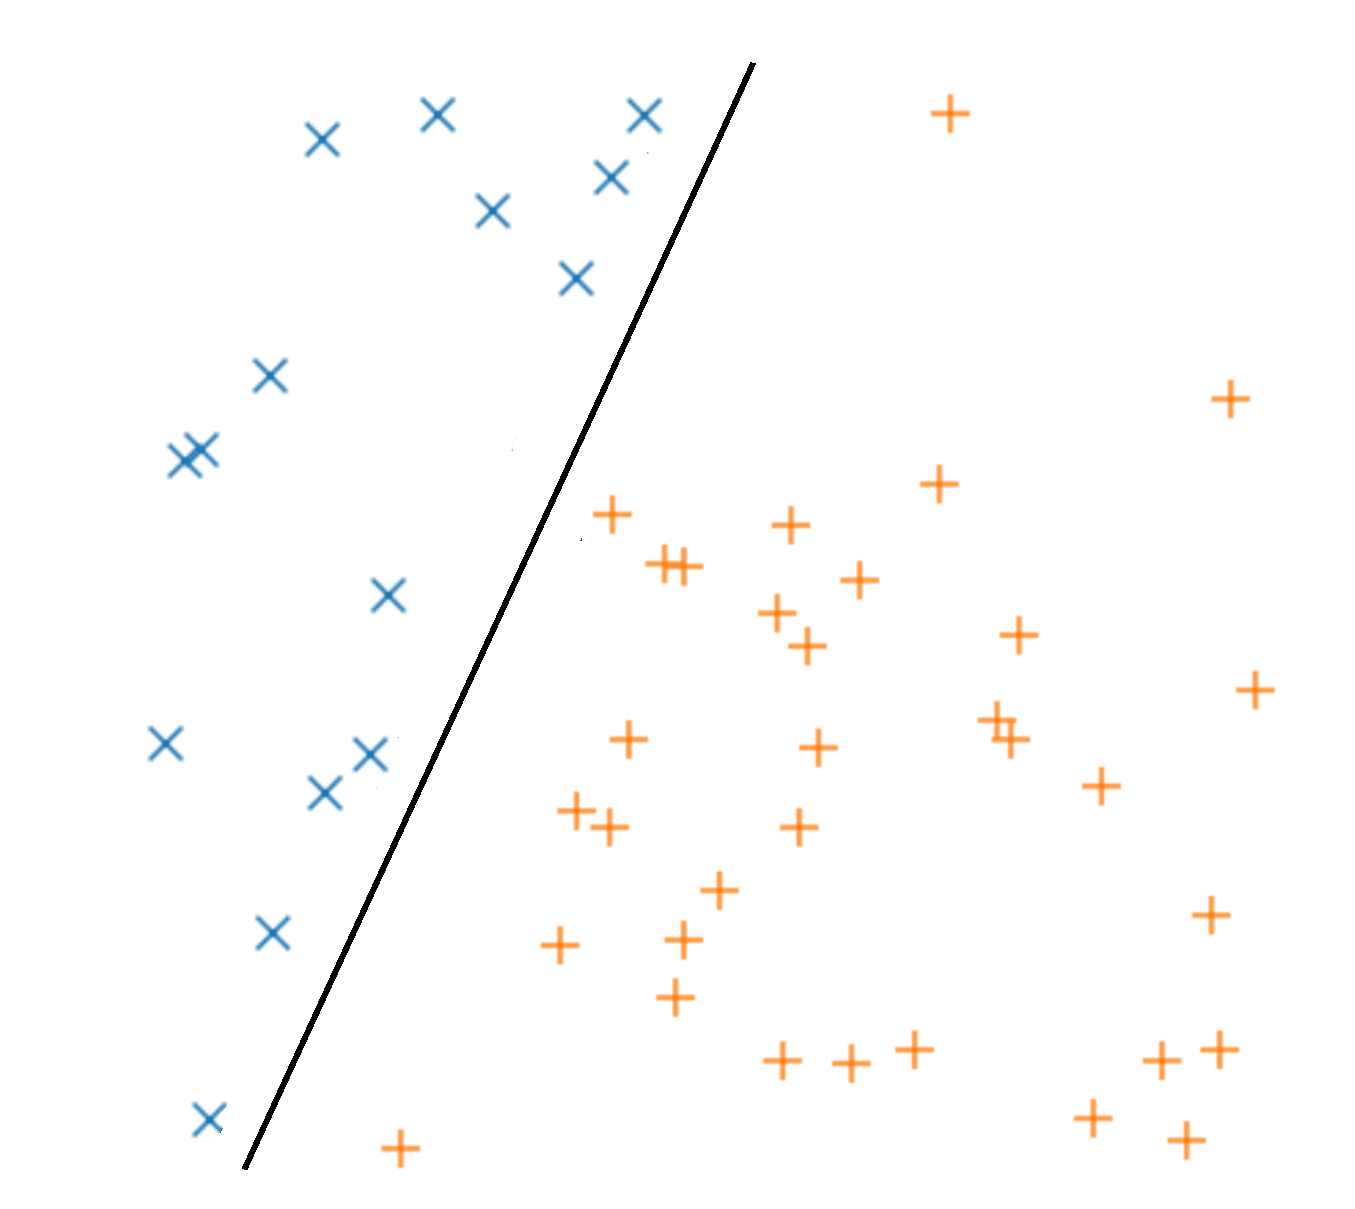
\includegraphics[width=0.4\textwidth,clip]{separabledroite.pdf}};
		\node (wiki)[]  at([yshift = 13]ref.north) {Linéairement séparables};
		%
		\node (ref1) [right=of ref,visible on=<2-3>] {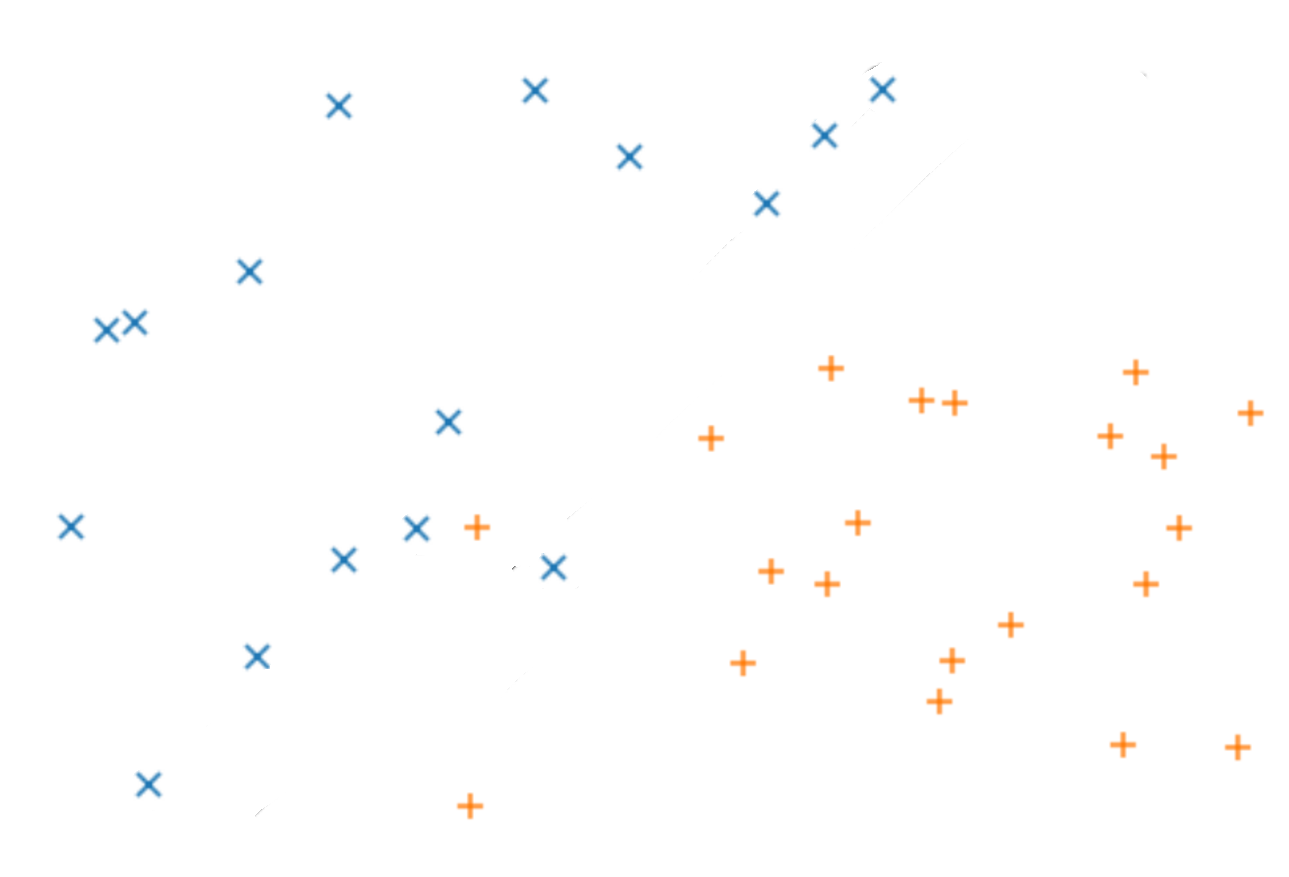
\includegraphics[width=0.4\textwidth,clip]{nonseparable.pdf}};
		\node (ref1) [right=of ref,visible on=<4>] {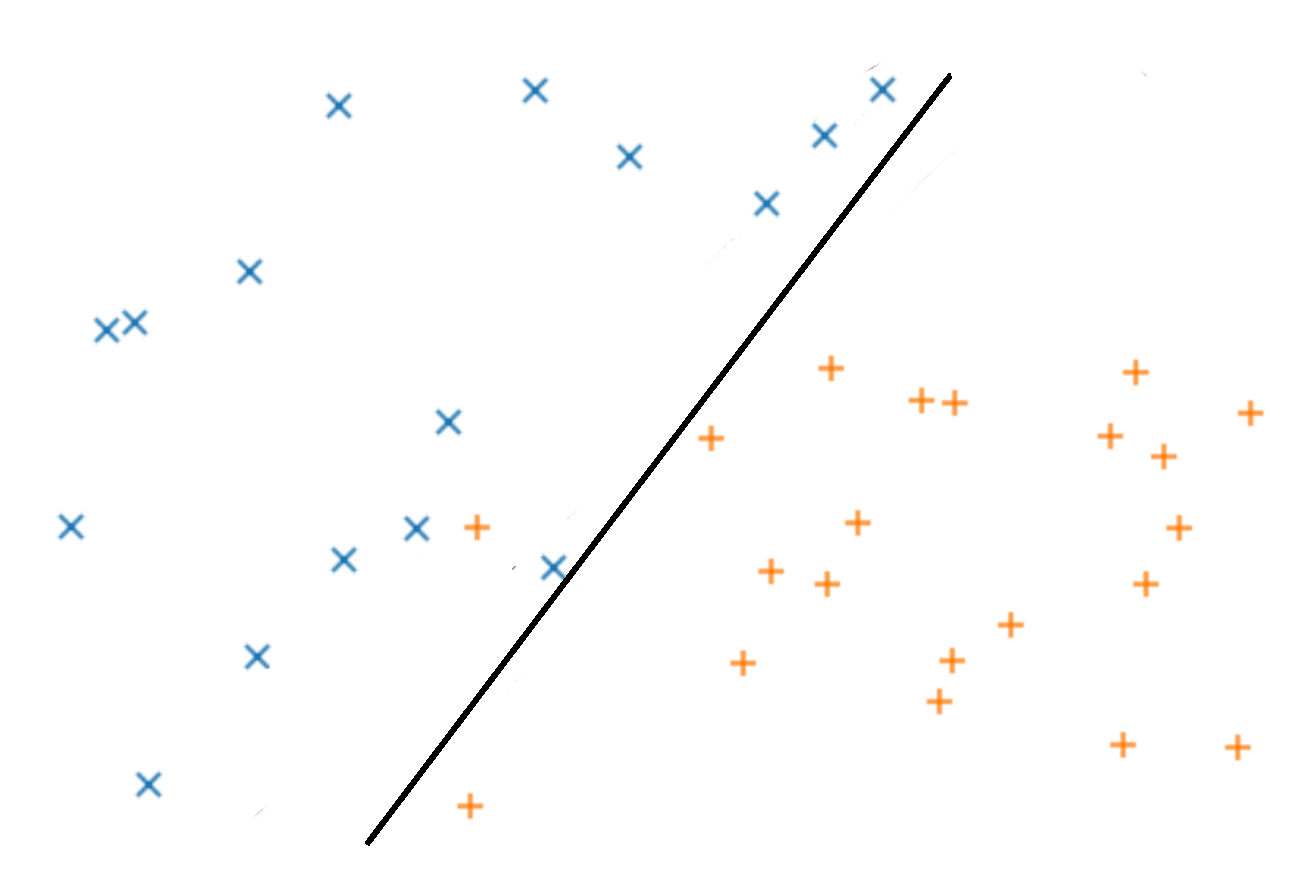
\includegraphics[width=0.4\textwidth,clip]{nonseparable1b.pdf}};
				\node (ref1) [right=of ref,visible on=<5>] {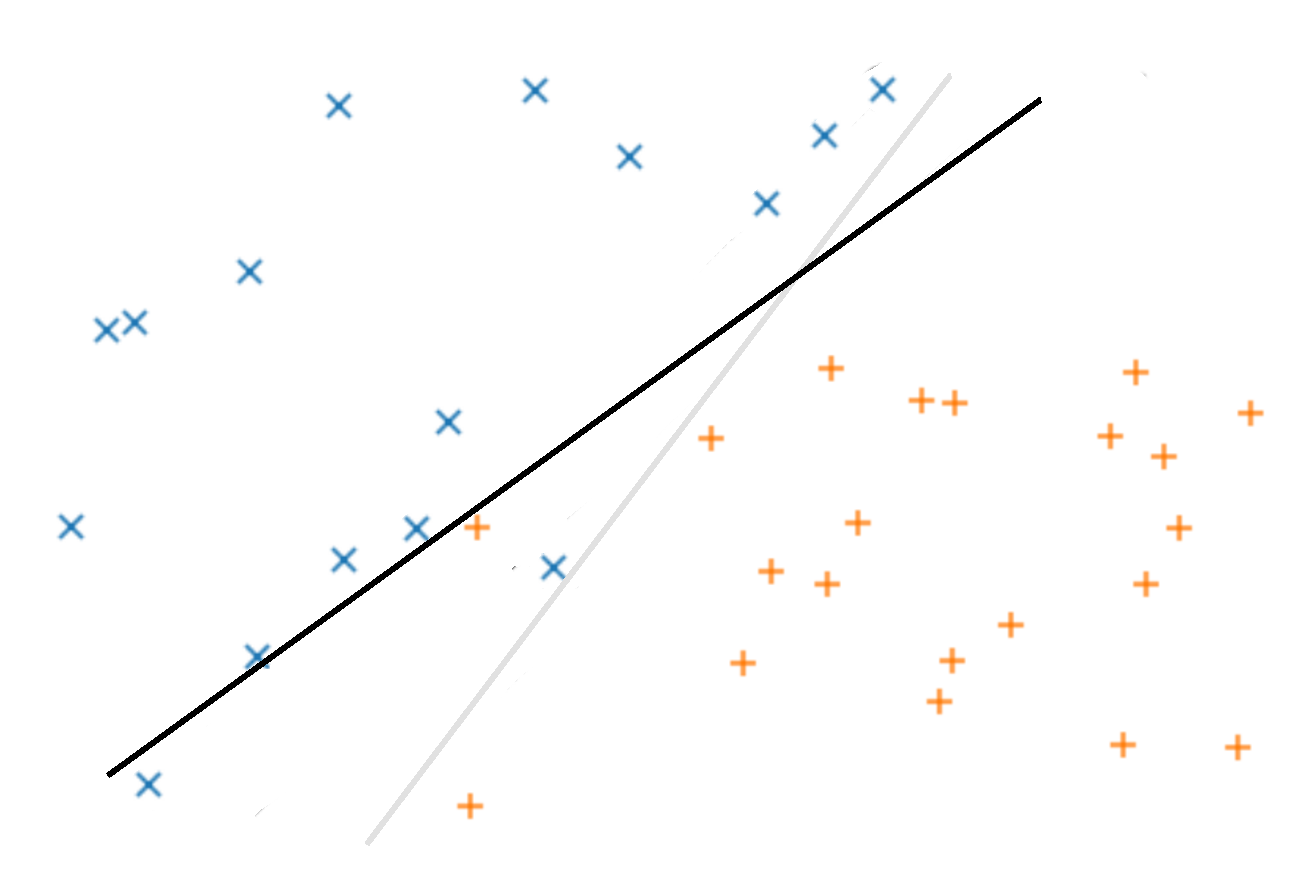
\includegraphics[width=0.4\textwidth,clip]{nonseparable2b.pdf}};
						\node (ref1) [right=of ref,visible on=<6>] {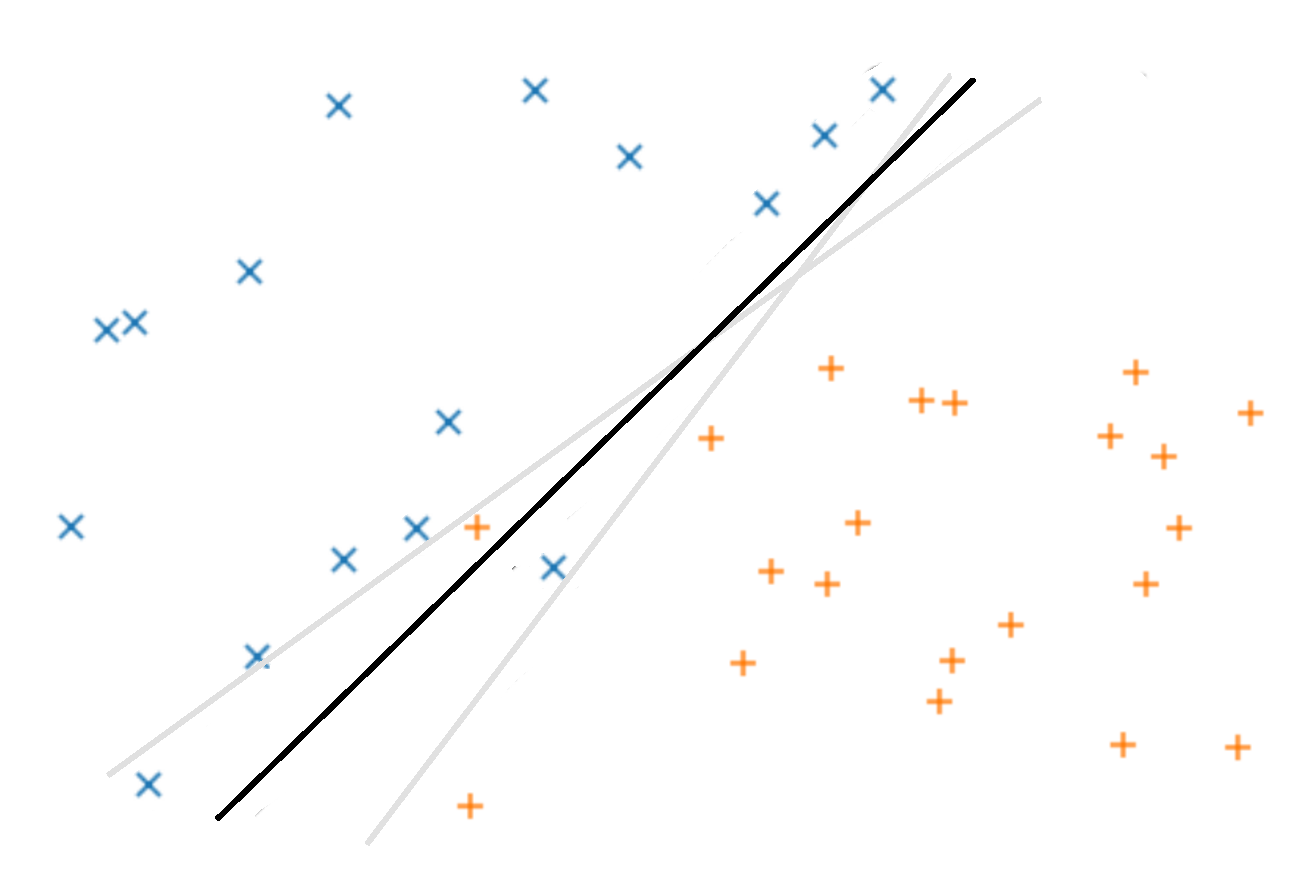
\includegraphics[width=0.4\textwidth,clip]{nonseparable3b.pdf}};
		%\node (wiki1)[]at([xshift = 30]wiki.east) {Non séparable linéairement};
		\node (wiki)[]  at([yshift = 27.5]ref1.north) {Non séparables linéairement};
		
	\end{tikzpicture}
	
\vspace*{1.5em}
\footnotesize{\textcolor{MPTgrey}{Tirée de l'ouvrage \textit{\href{http://cazencott.info/dotclear/public/lectures/IntroML_Azencott.pdf}{Introduction au Machine Learning}} de Chloé-Agathe Azencott} }
	
\end{center}
\end{frame}

%------------------------------------------------------------------------------------------
%------------------------------------------------------------------------------------------



\section{Le cas linéairement séparable :\\[0.5em] SVM à marge rigide}



%------------------------------------------------------------------------------------------
%------------------------------------------------------------------------------------------
\begin{frame}{Séparabilité linéaire}
	
	\textcolor{MPTblue}{\large\textbf{Définition}}	
	\begin{vblock}{}
		Un jeu de données $\left\{(x_i,y_i)\right\}_{i=1,\dots,n}$ est \textbf{linéairement séparable} s'il existe au moins un hyperplan dans $\bbR^d$ tel que tous les points $x_i$ positifs ($y_i=1$) sont \hsp \\d'un côté de cet hyperplan et tous les points $x_i$ négatifs ($y_i=-1$) de l'autre
	\end{vblock}
	
	%\vspace*{2em}
	\begin{minipt}[0.48]{0.7}
		%	\begin{center}
			\begin{tikzpicture}
				\node (ref) [visible on=<1>] {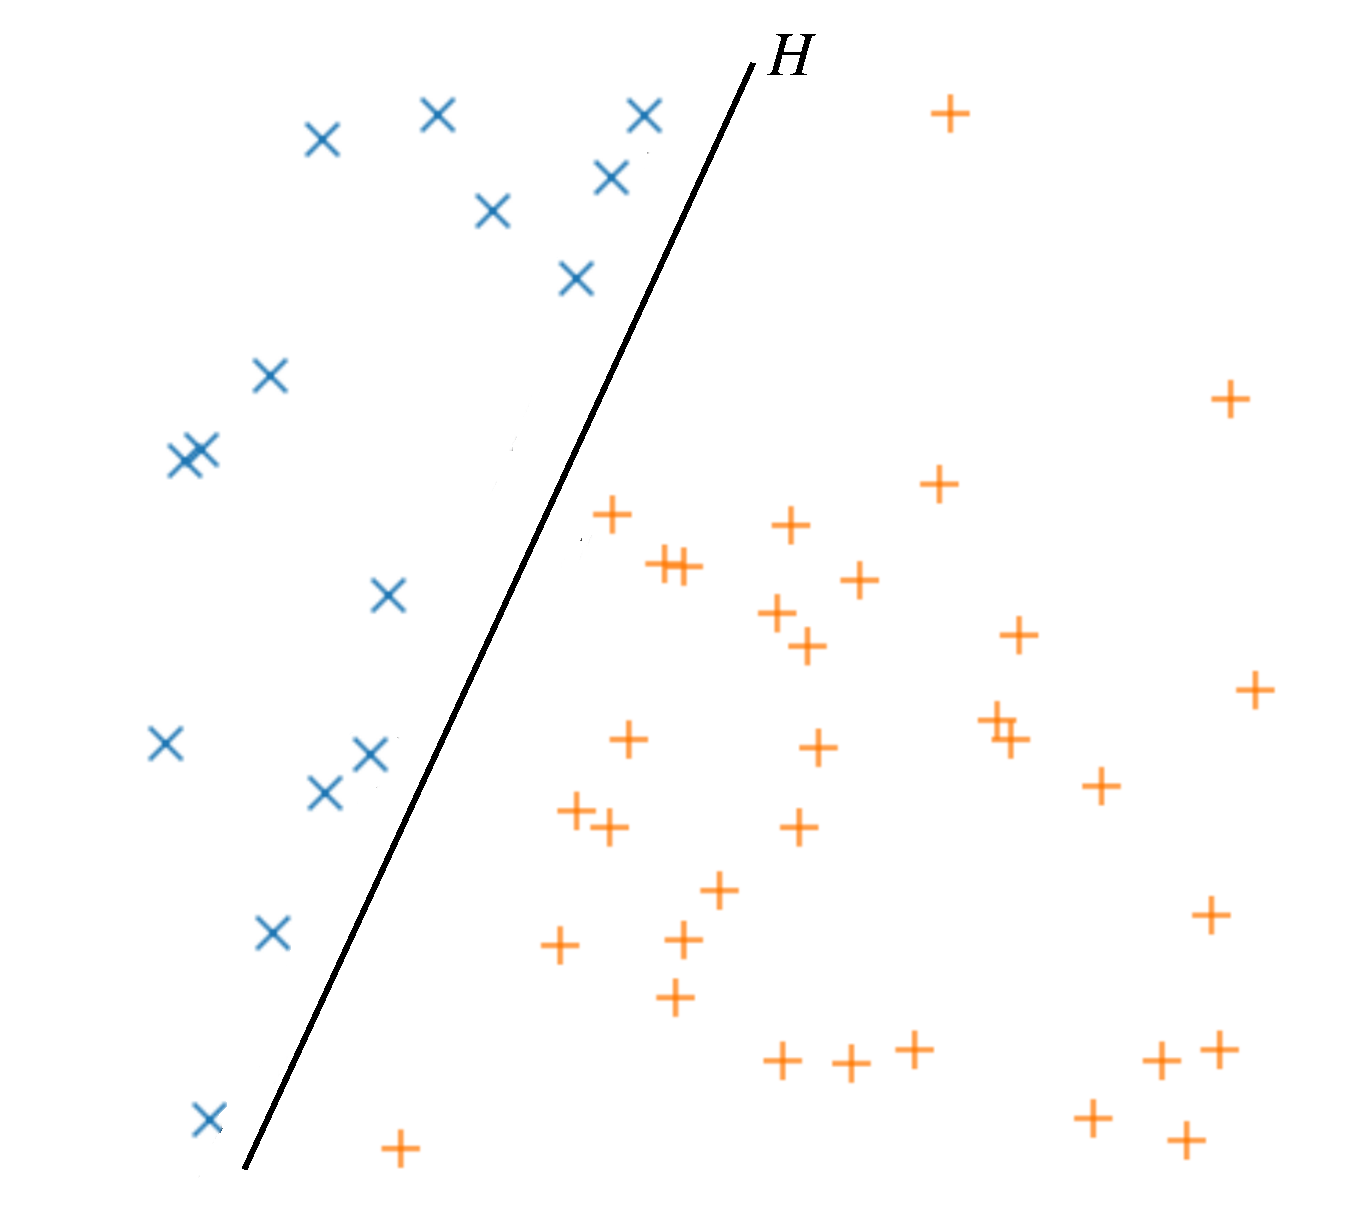
\includegraphics[width=1\textwidth,clip]{separabledroiteb1.pdf}};
				\node (ref) [visible on=<2-4>] {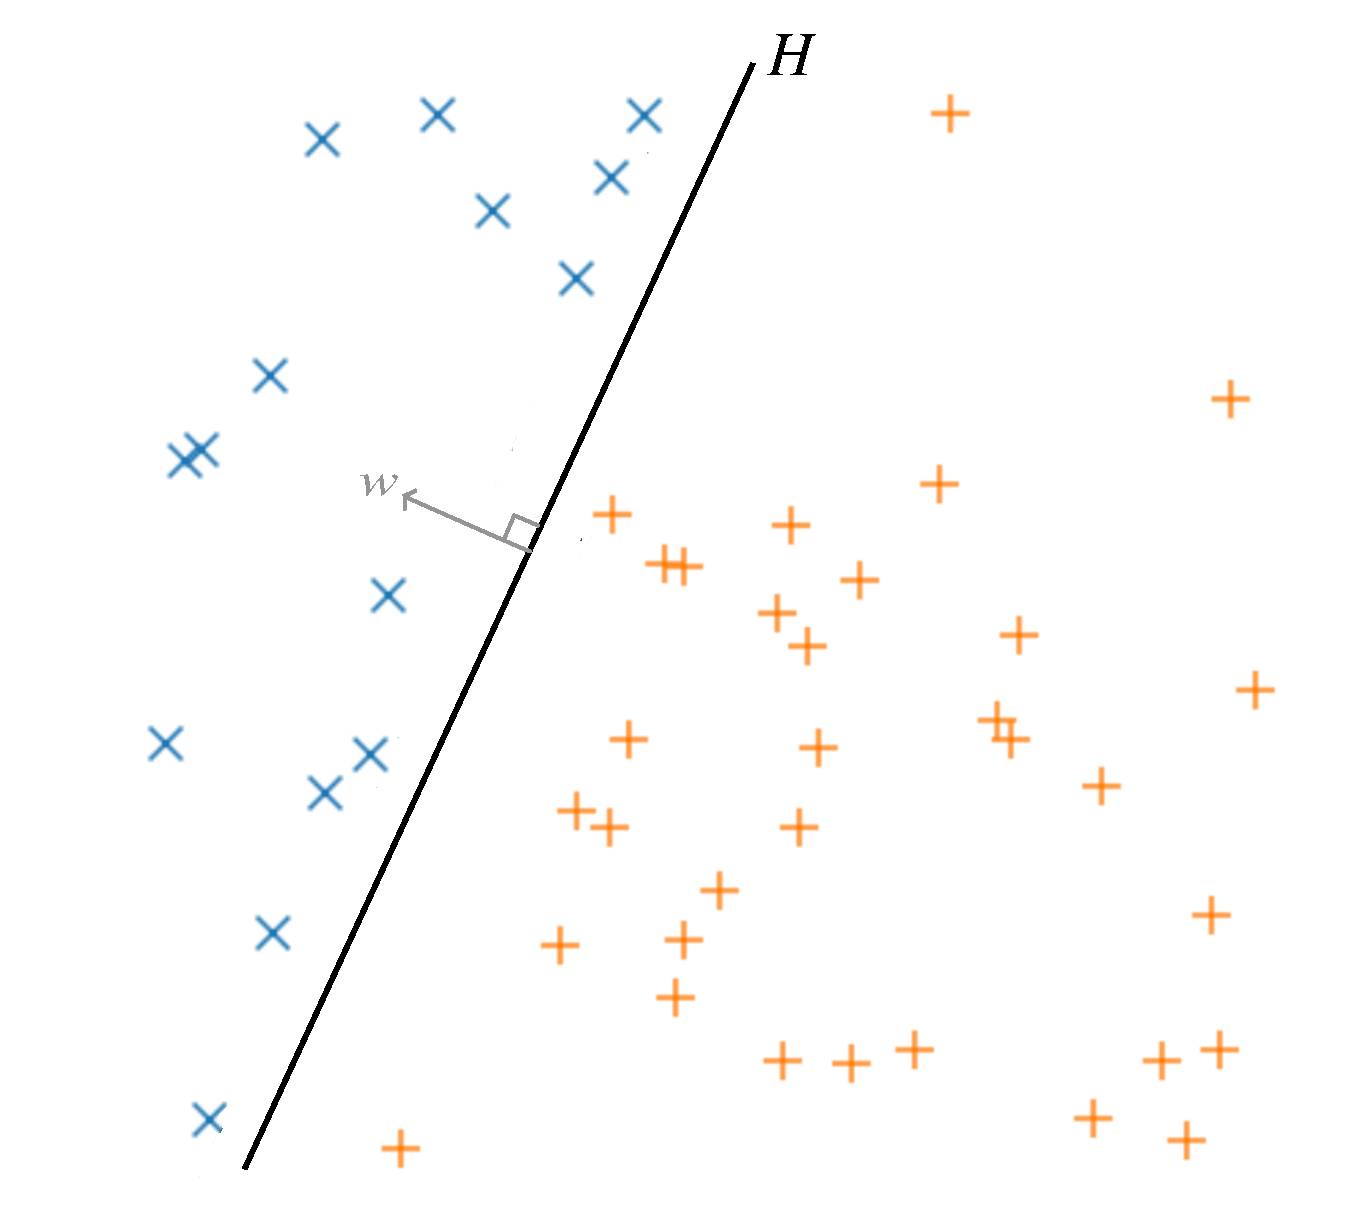
\includegraphics[width=1\textwidth,clip]{separabledroiteb2.pdf}};
				%\node (ref) [visible on=<3>] {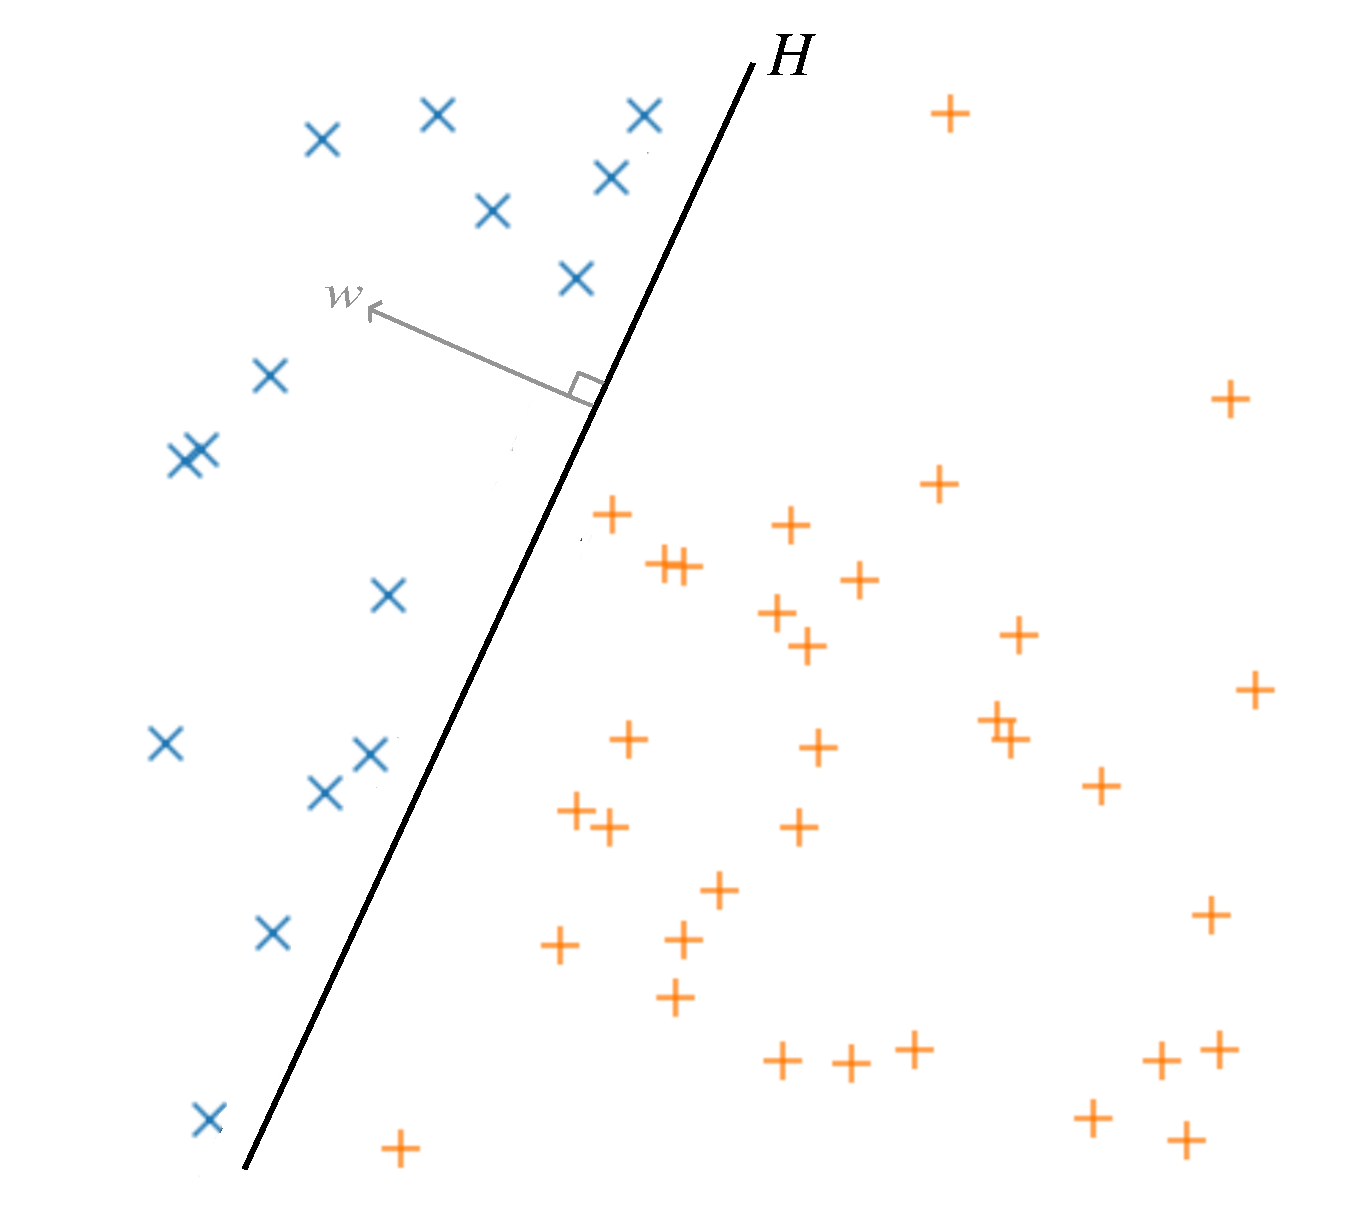
\includegraphics[width=1\textwidth,clip]{separabledroiteb3.pdf}};
			%	\node (ref) [visible on=<4>] {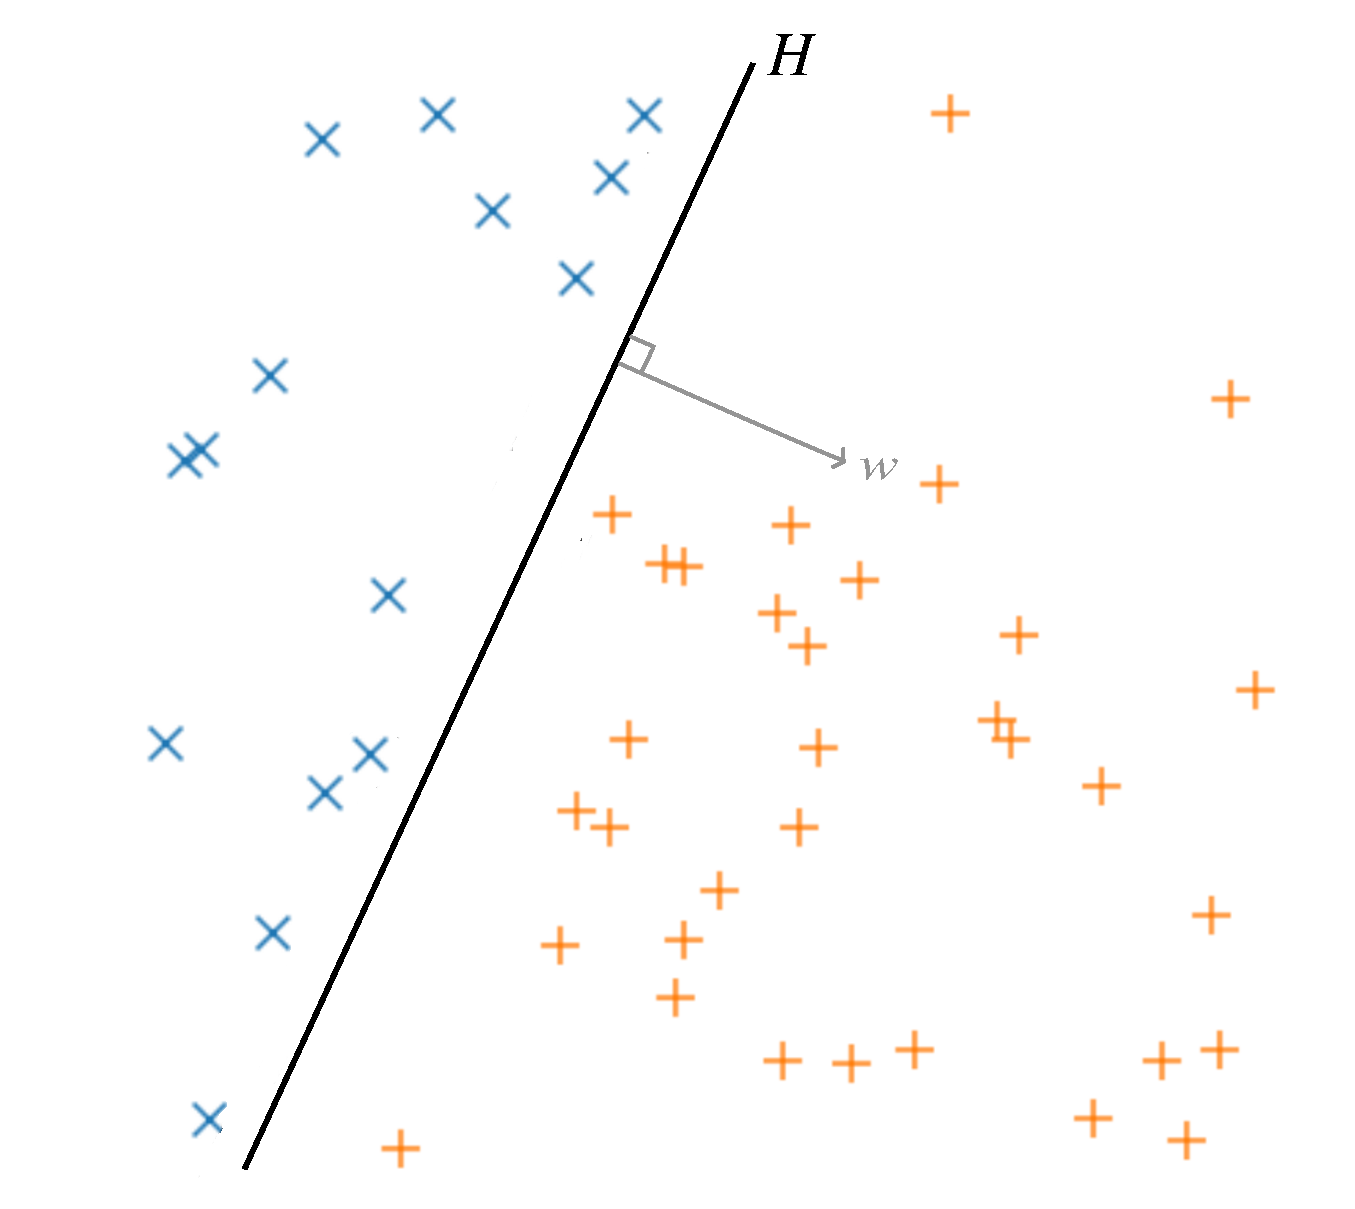
\includegraphics[width=1\textwidth,clip]{separabledroiteb4.pdf}};
				%\node (ref) [visible on=<5>] {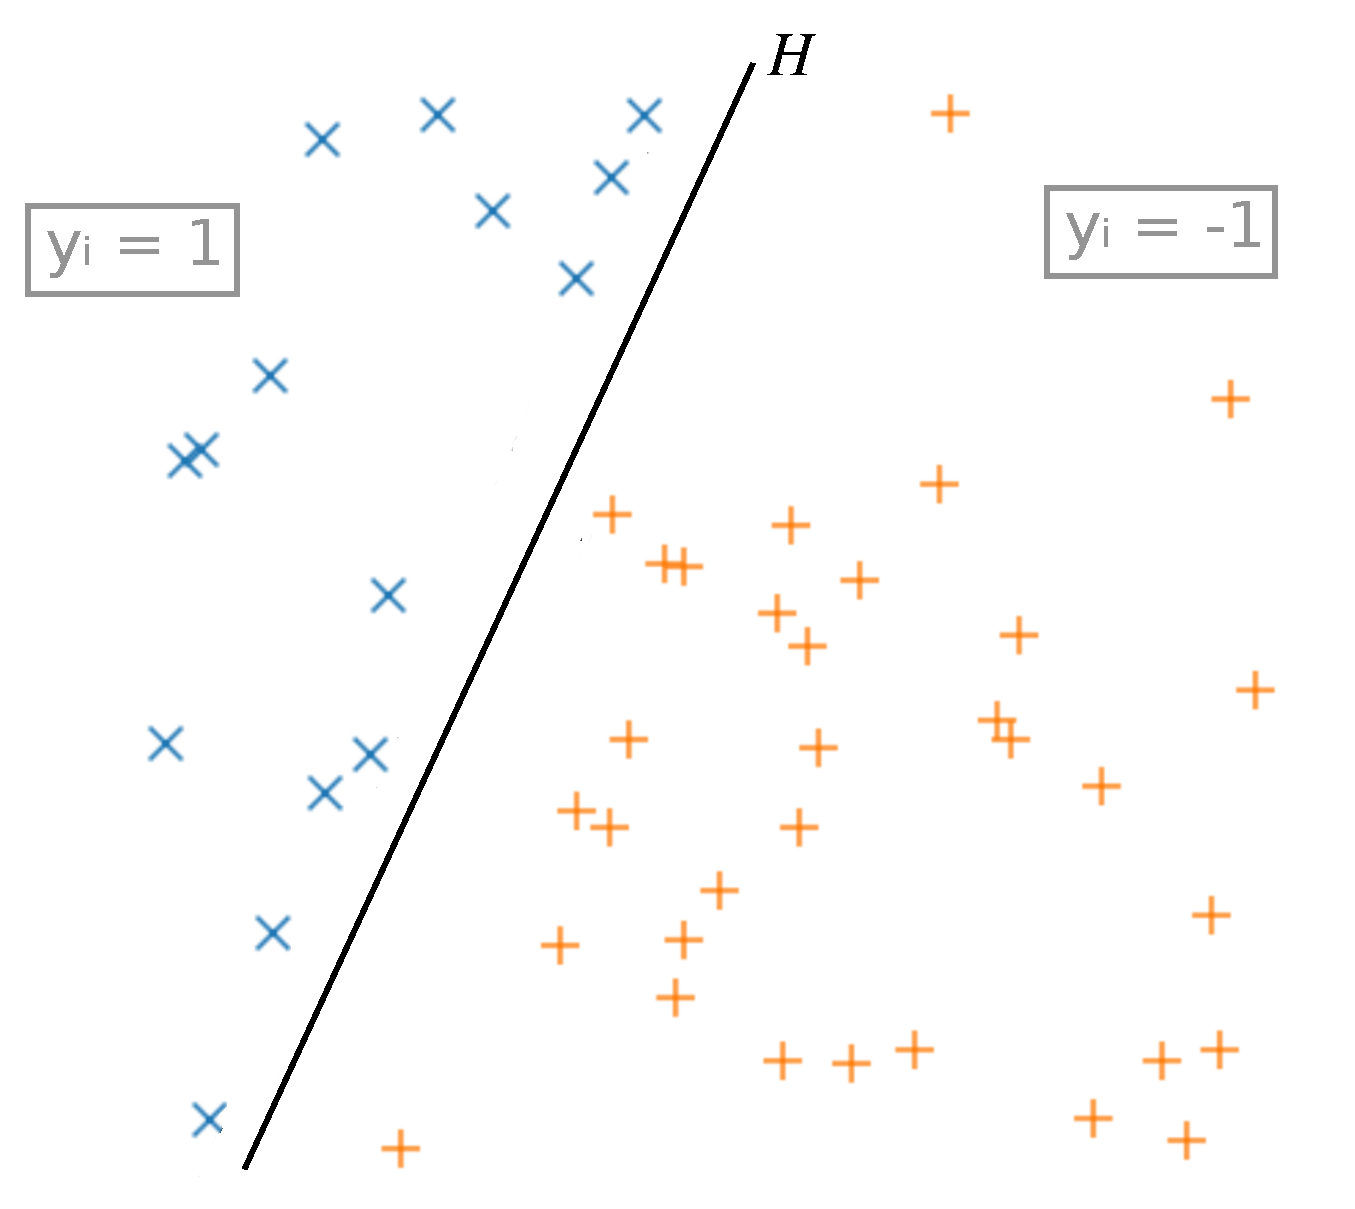
\includegraphics[width=1\textwidth,clip]{separabledroiteb5.pdf}};
				%\node (ref) [visible on=<6>] {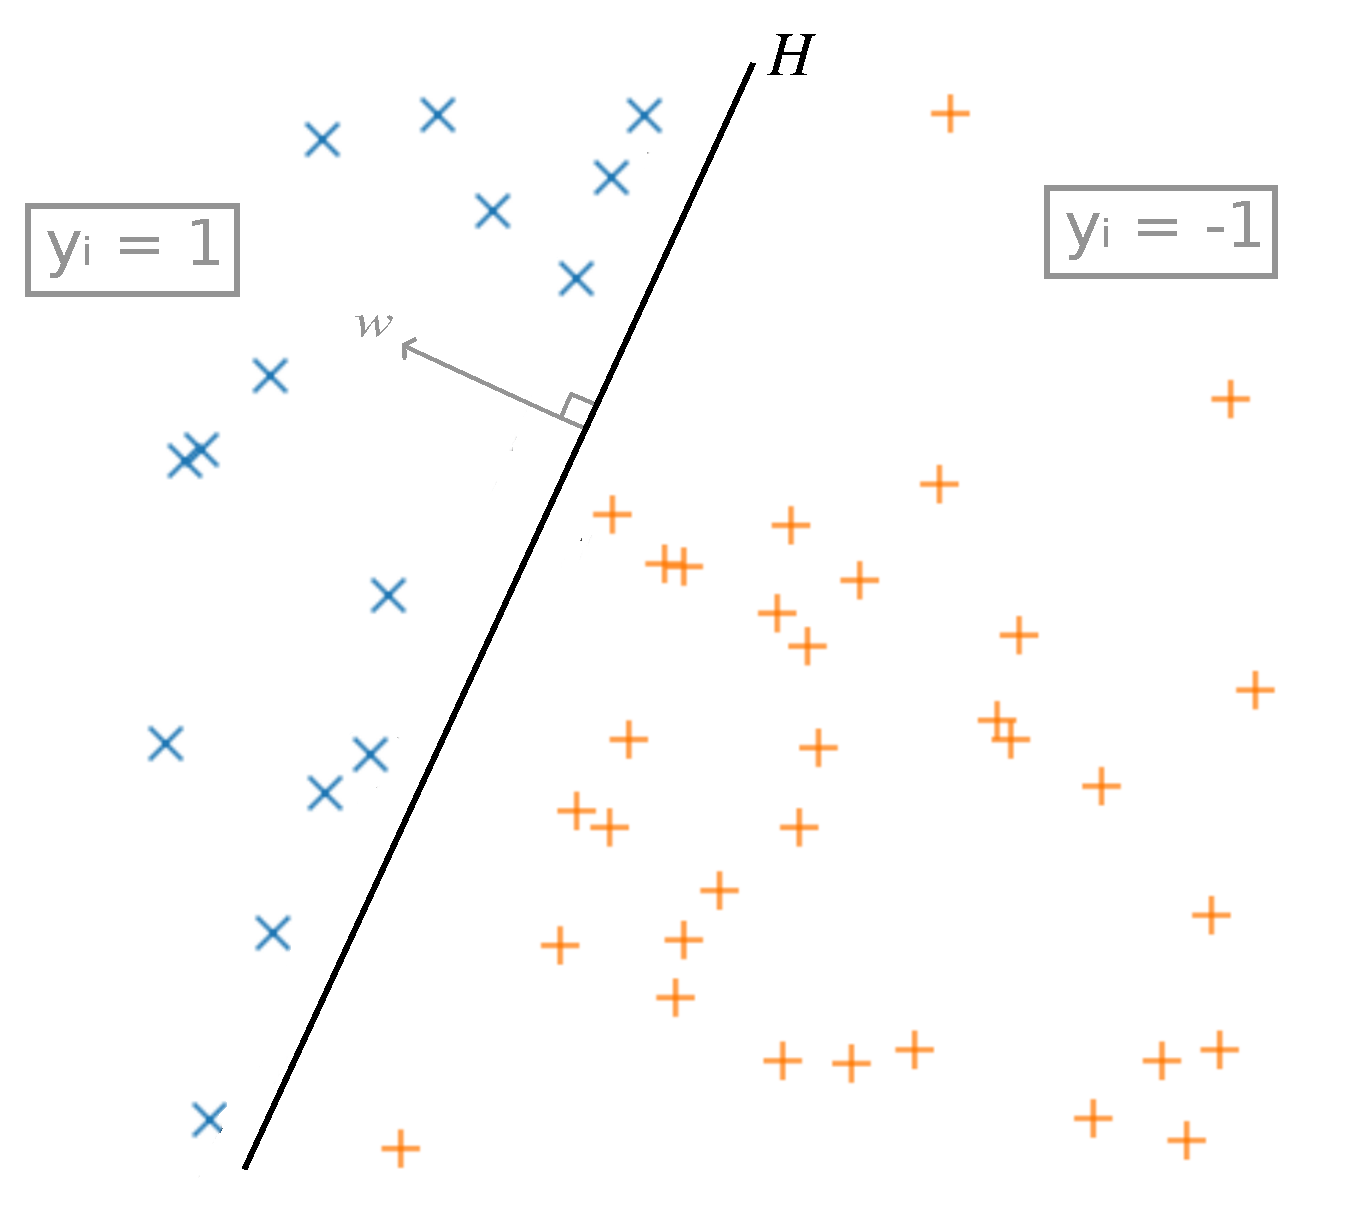
\includegraphics[width=1\textwidth,clip]{separabledroiteb11.pdf}};
			%	\node (ref) [visible on=<7>] {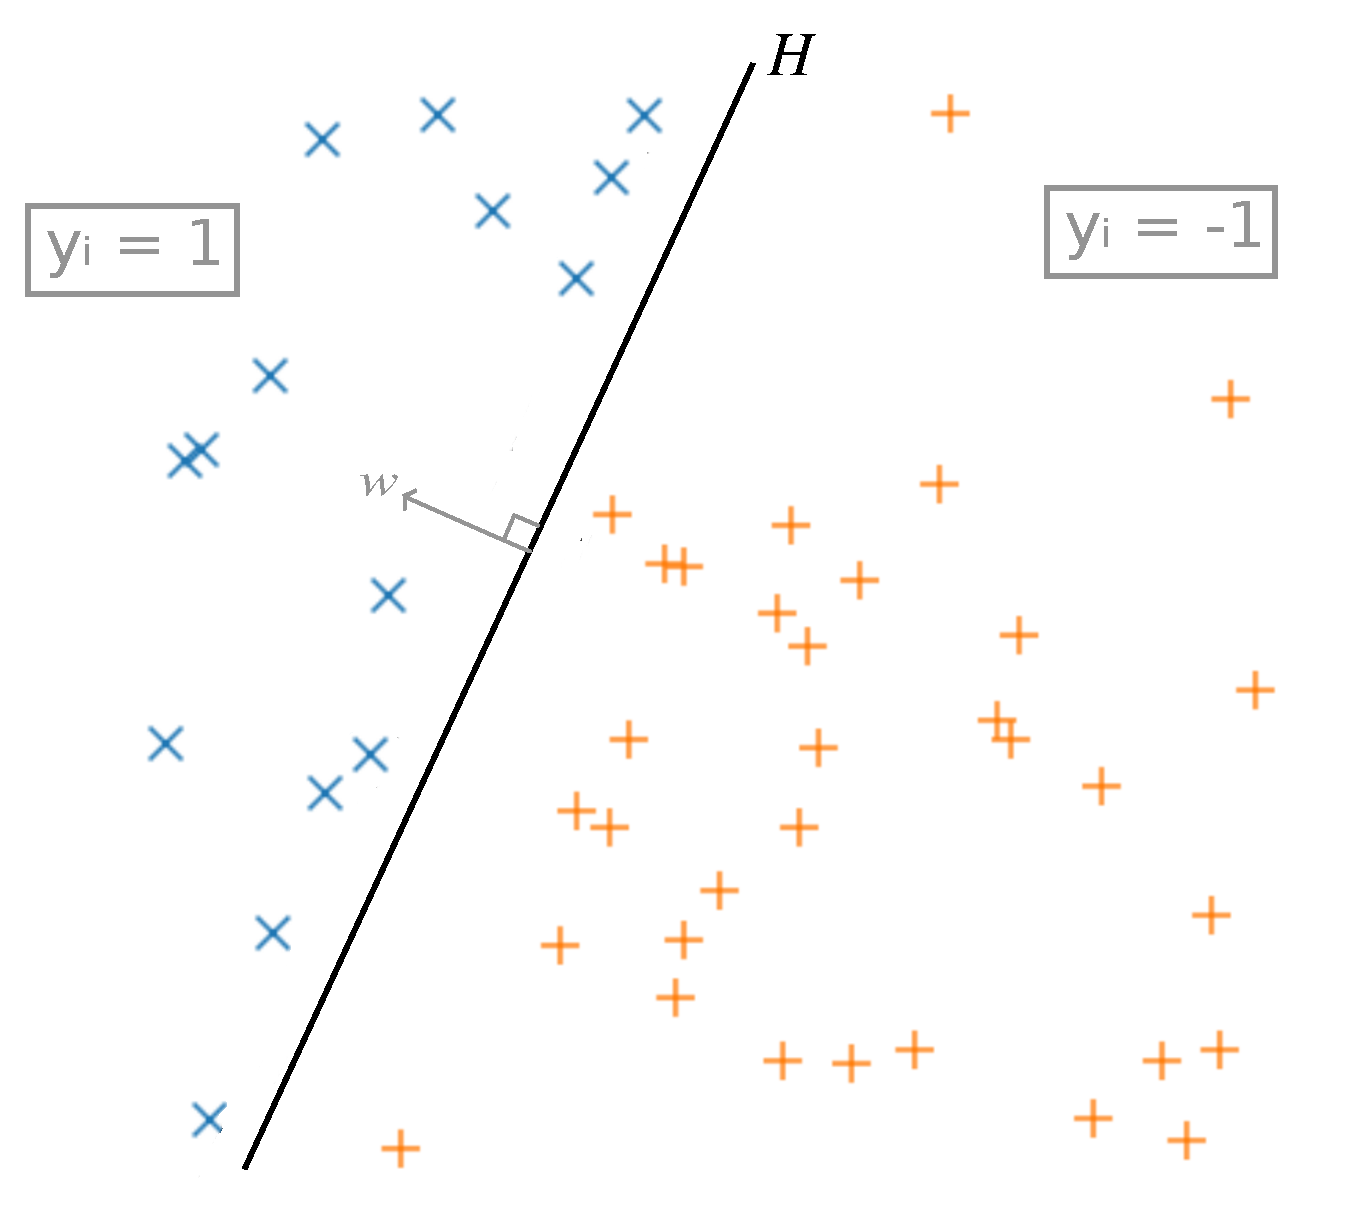
\includegraphics[width=1\textwidth,clip]{separabledroiteb6.pdf}};
			%	\node (ref) [visible on=<5>] {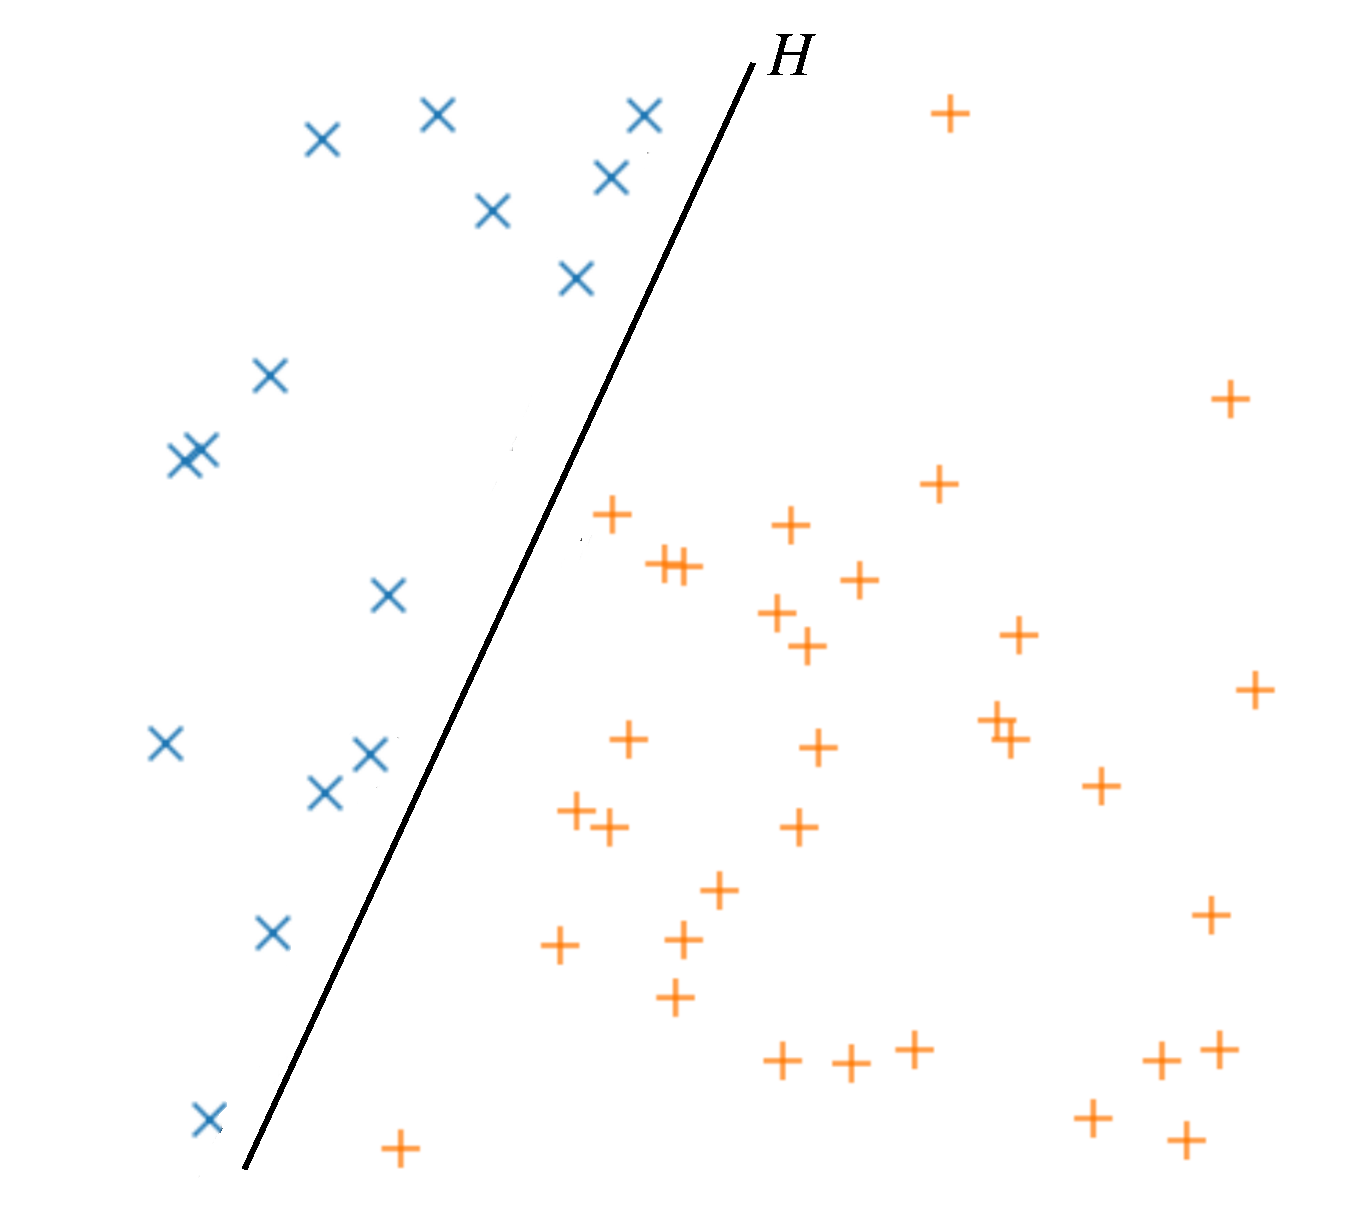
\includegraphics[width=1\textwidth,clip]{separabledroiteb1.pdf}};
				\node (ref) [visible on=<5>] {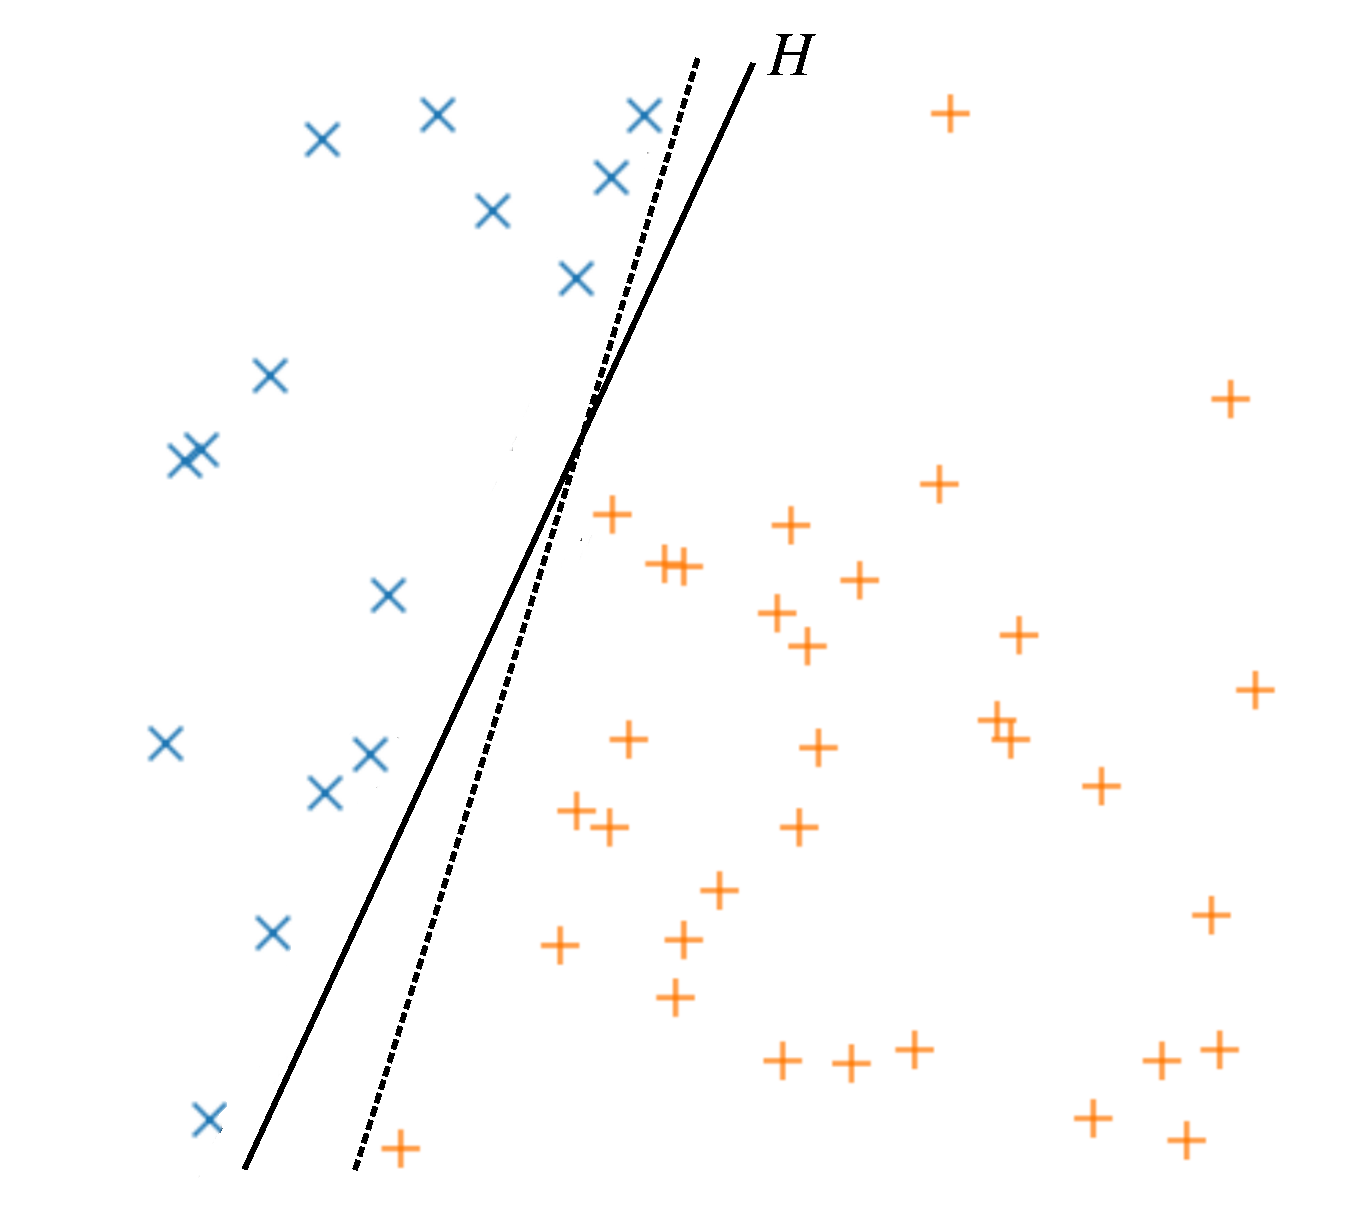
\includegraphics[width=1\textwidth,clip]{separabledroiteb7.pdf}};
				\node (ref) [visible on=<6>] {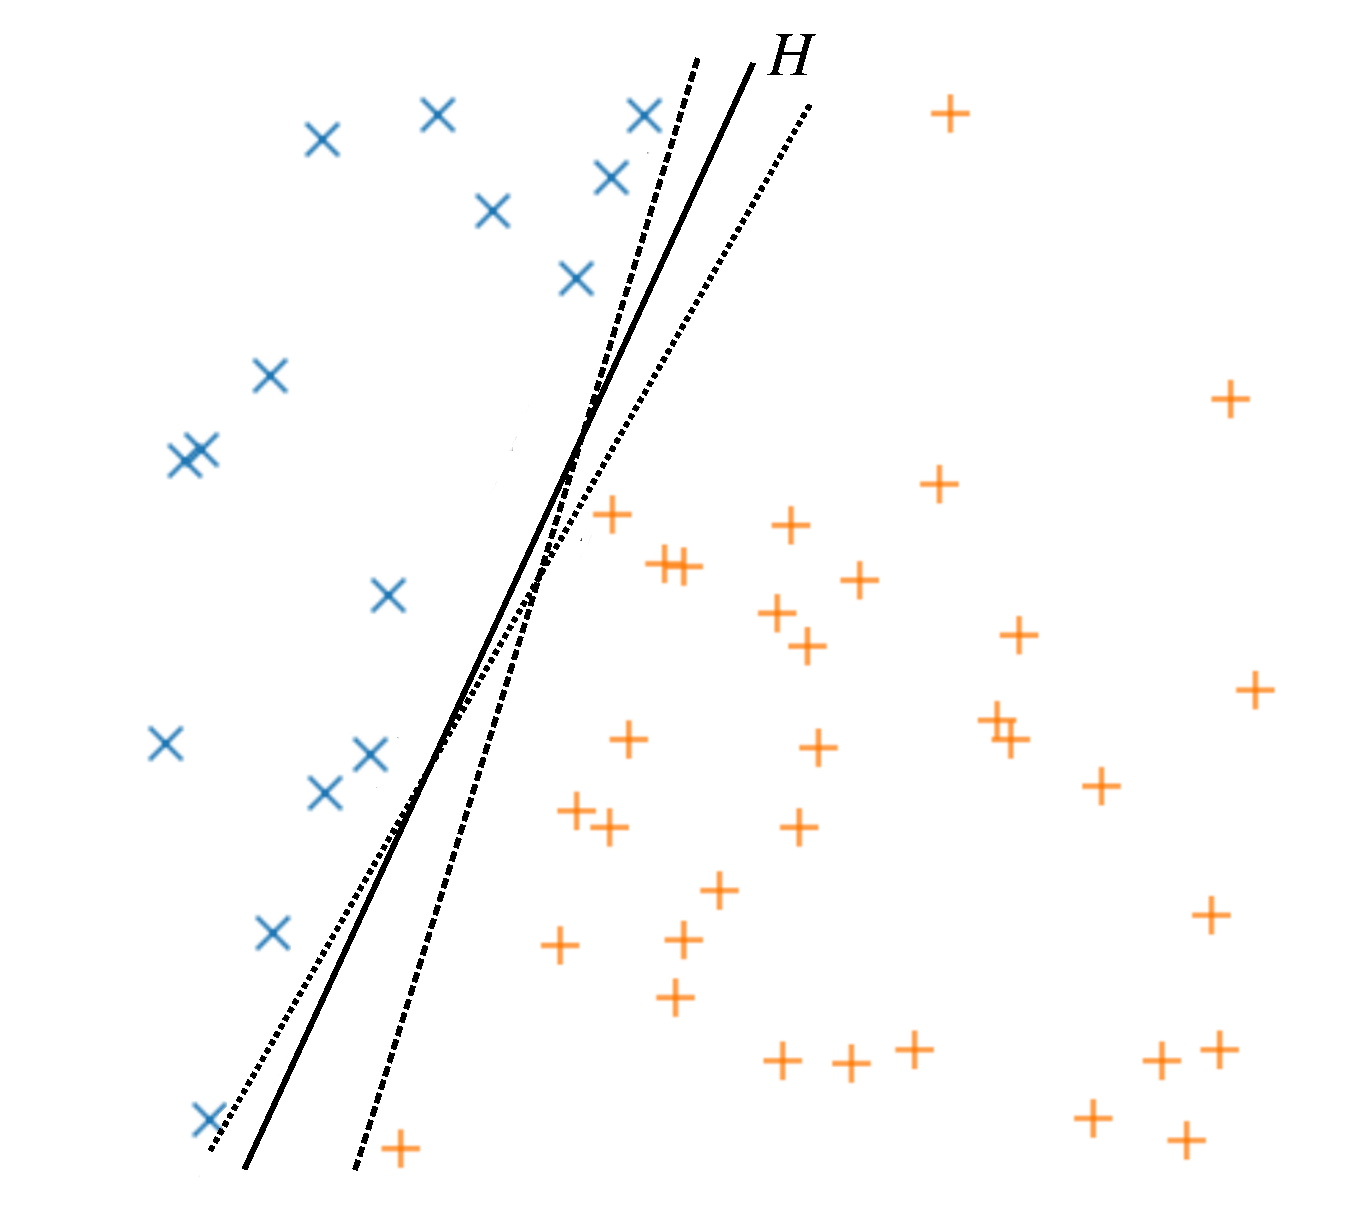
\includegraphics[width=1\textwidth,clip]{separabledroiteb8.pdf}};
				\node (ref) [visible on=<7-8>] {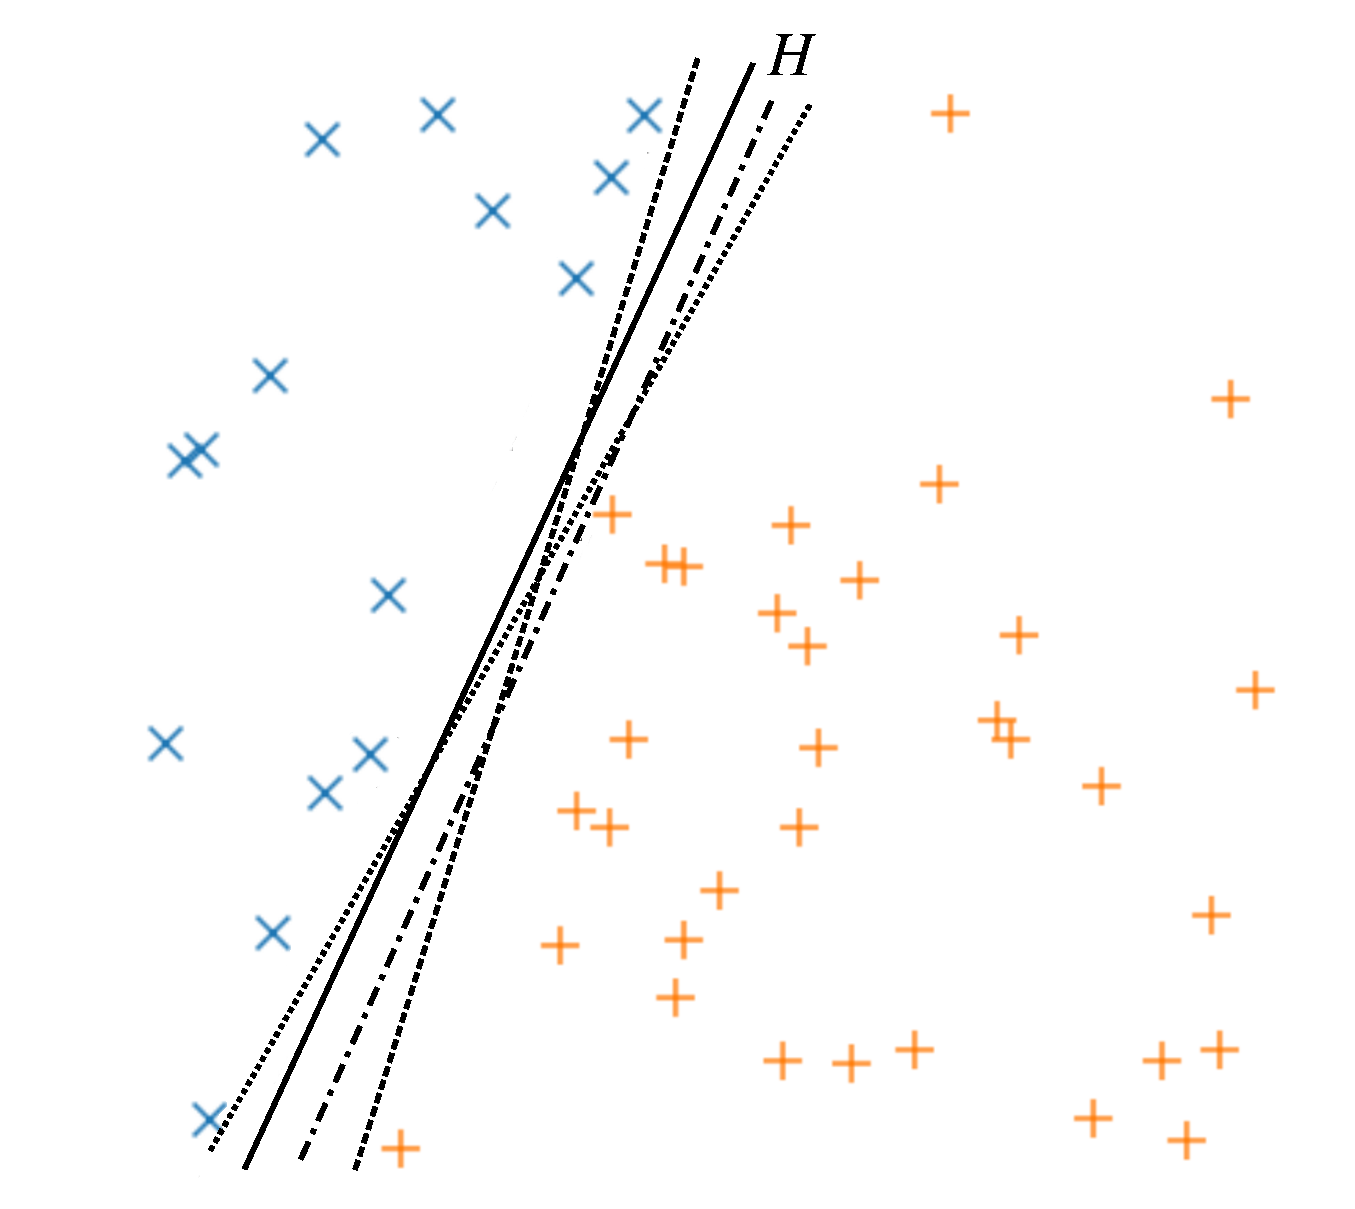
\includegraphics[width=1\textwidth,clip]{separabledroiteb9.pdf}};
				\node (ref) [visible on=<9-10>] {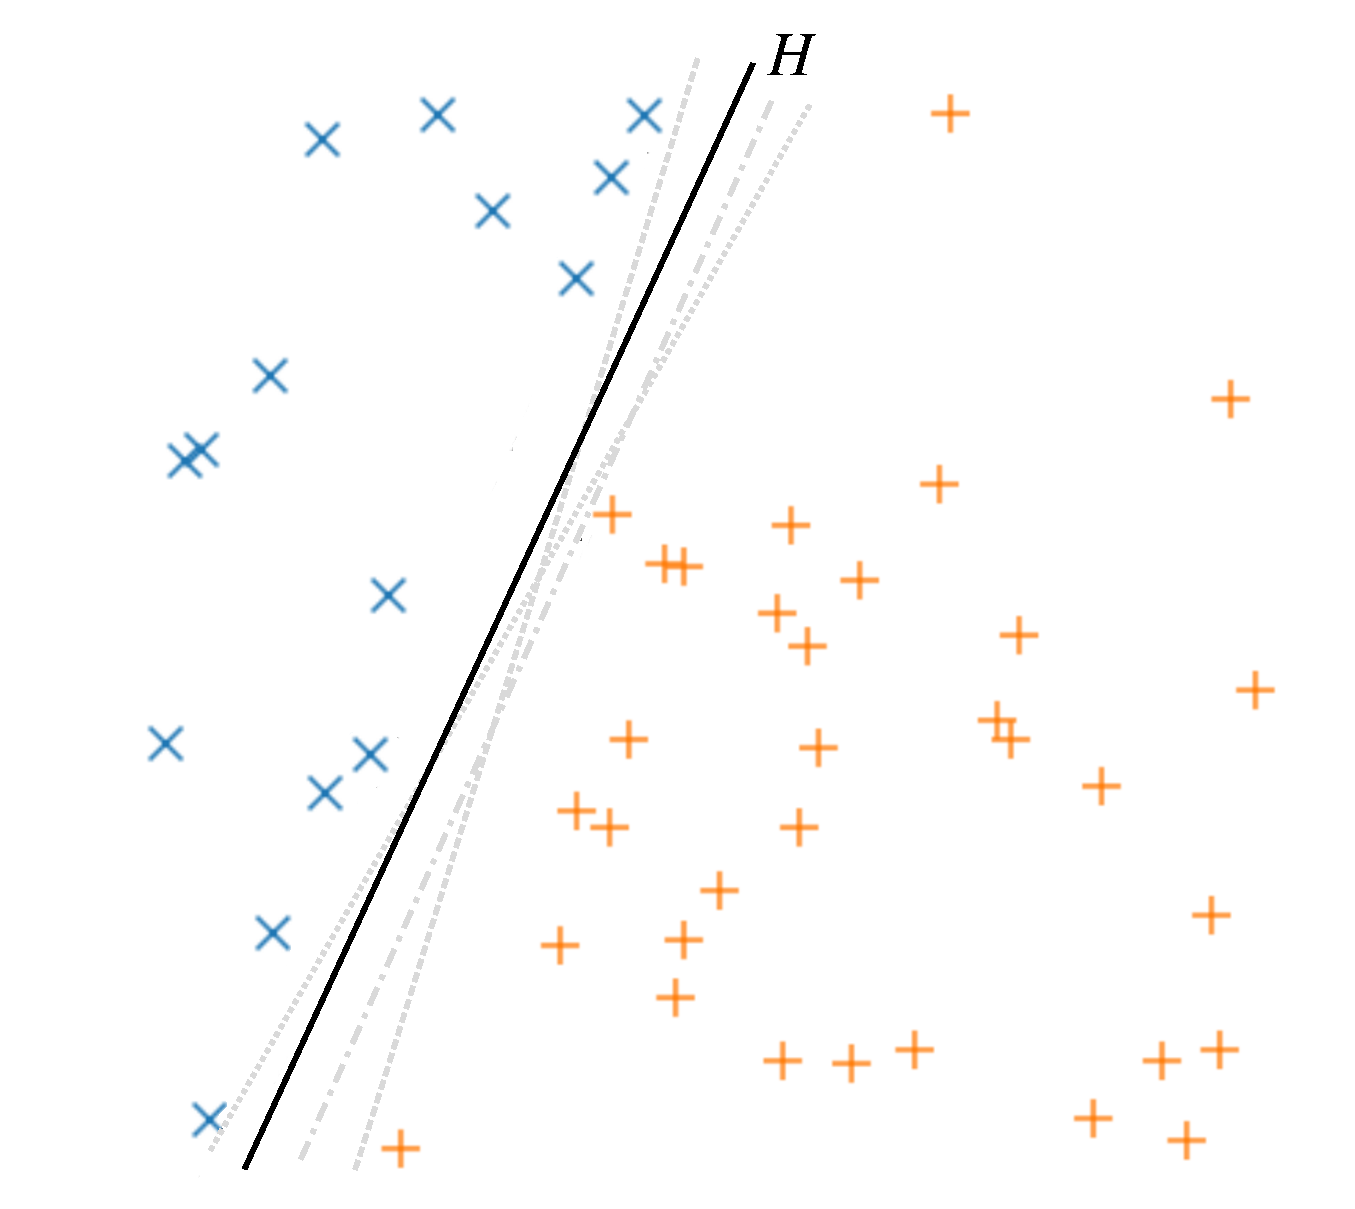
\includegraphics[width=1\textwidth,clip]{separabledroiteb10.pdf}};
			\end{tikzpicture}
		\end{minipt}
		\hfill
			\begin{minipt}[0.48]{0.75}
					\vspace*{-14.9em}
		\begin{minipt}[1]{0.18}
			
				
			%	$$ \dfrac{1}{n} \sum_{i=1}^n  $$
			%
			\end{minipt}
			\only<2-7>{	\begin{minipt}[1]{0.56}
					\vspace*{-0.5em}
			%\vspace*{-14.9em}
			Équation de $H$ : $\langle w,x\rangle+ b = 0$\\ 
			$\color{MPTgrey} (w,b) \in \bbR^{d} \times \bbR$ \textcolor{MPTgrey}{avec} $ \color{MPTgrey} \vec{w} \perp H$  \\[0.2em]					
			%Plusieurs solutions pour $(\beta,\beta_0)$ : 
			\textcolor{MPTgrey}{0n choisit $\color{MPTgrey}(w,b)$ tel que l'angle entre $\color{MPTgrey}\vec{w}$ et tout point positif est inférieur à $\color{MPTgrey}90^\circ$}\\[0.5em]		 
	 \only<3-7>{Pour tout nouveau point $x$, on estime son label $y$ par $\text{sign} \left[\langle w,x \rangle+ b \right]$\\}
	 %$\forall i \in \{1,\dots,n\} \, \text{sign} \left[\langle w,x_i \rangle+ b \right] = y_i$\\		% $\dfrac{1}{n} \sum_{i=1}^n  \mathbb{1} \left\{\text{sign} \left[\langle \beta,x_i \rangle+ \beta_0 \right] \neq y_i \right\}= 0$\\	
	 \only<4-7>{		
	 	
	 	Un hyperplan séparateur $H$ ne fait aucune erreur de classification sur les données d'apprentissage\\[0.7em]		 
			 \ex \ $(w,b) $ minimise le risque empirique pour le coût 0/1 $\color{MPTgrey} \rightarrow$ \textcolor{MPTgrey}{candidat pour} $\color{MPTgrey}(\widehat{w},\widehat{b})$}
				\end{minipt}
			}
			
			\only<8->{
				\vspace*{-5em}	\uncover<8->{
				\begin{minipc}[0.13]{0.16}
					\warning
				\end{minipc}
				\begin{minipc}[0.82]{0.16}
					Il existe une infinité d'hyperplans séparateurs
				\end{minipc}
			}
			
		%	\vspace{1em}
			\uncover<9->{
				\begin{minipc}[0.13]{0.2}
					\raisebox{1.5mm}{\bclampe \xspace} 
				\end{minipc}
				\begin{minipc}[0.82]{0.2}
					On cherche l'hyperplan dont la distance à l'observation la plus proche est la plus grande possible %\hsp \textcolor{MPTgrey}{(Pourquoi ?)^}
				\end{minipc}
			}
		\uncover<10>{
			\begin{minipc}[0.13]{0.2}
			\phantom{	\raisebox{1.5mm}{\bclampe \xspace}} 
			\end{minipc}
		\begin{minipc}[0.82]{0.2}
			Cet observation sera donc à équidistance des observations positive et négative les plus proches
	\end{minipc} }
			}
					
			\end{minipt}	
		%------------------------NOTE
		\note{On idée pour savoir comment on choisit l'hyperplan}
		
\end{frame}
%------------------------------------------------------------------------------------------
\begin{frame}
	
	L'hyperplan équidistant des observations positive et négative les plus proches permet de ne pas être sensible à un petit changement dans les données (permet de mieux gérer les erreurs de mesure par exemple). \\[2em]
	
	\begin{center}
		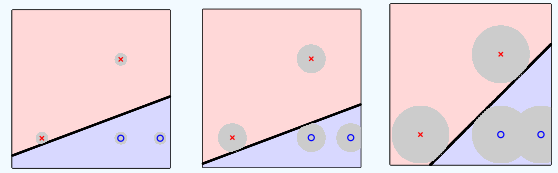
\includegraphics[width=0.9\textwidth]{hyperplanbest.png}
		
		\vspace*{1.5em}
		\footnotesize{\textcolor{MPTgrey}{Tirée de  \textit{\href{https://edisciplinas.usp.br/pluginfile.php/5078086/course/section/5978681/chapSVM.pdf}{cet ouvrage}}} }
	\end{center}
\end{frame}
%------------------------------------------------------------------------------------------
%
%\begin{frame}{Séparabilité linéaire}
%	
%	\textcolor{MPTblue}{\large\textbf{Définition}}	
%	\begin{vblock}{}
%	Un jeu de données $\left\{(x_i,y_i)\right\}_{i=1,\dots,n}$ est \textbf{linéairement séparable} s'il existe au moins un hyperplan dans $\bbR^d$ tel que tous les points $x_i$ positifs ($y_i=1$) sont \hsp \\d'un côté de cet hyperplan et tous les points $x_i$ négatifs ($y_i=-1$) de l'autre
%	\end{vblock}
%
%	%\vspace*{2em}
%\begin{minipt}[0.48]{0.7}
%	%	\begin{center}
%		\begin{tikzpicture}
%				\node (ref) [visible on=<1>] {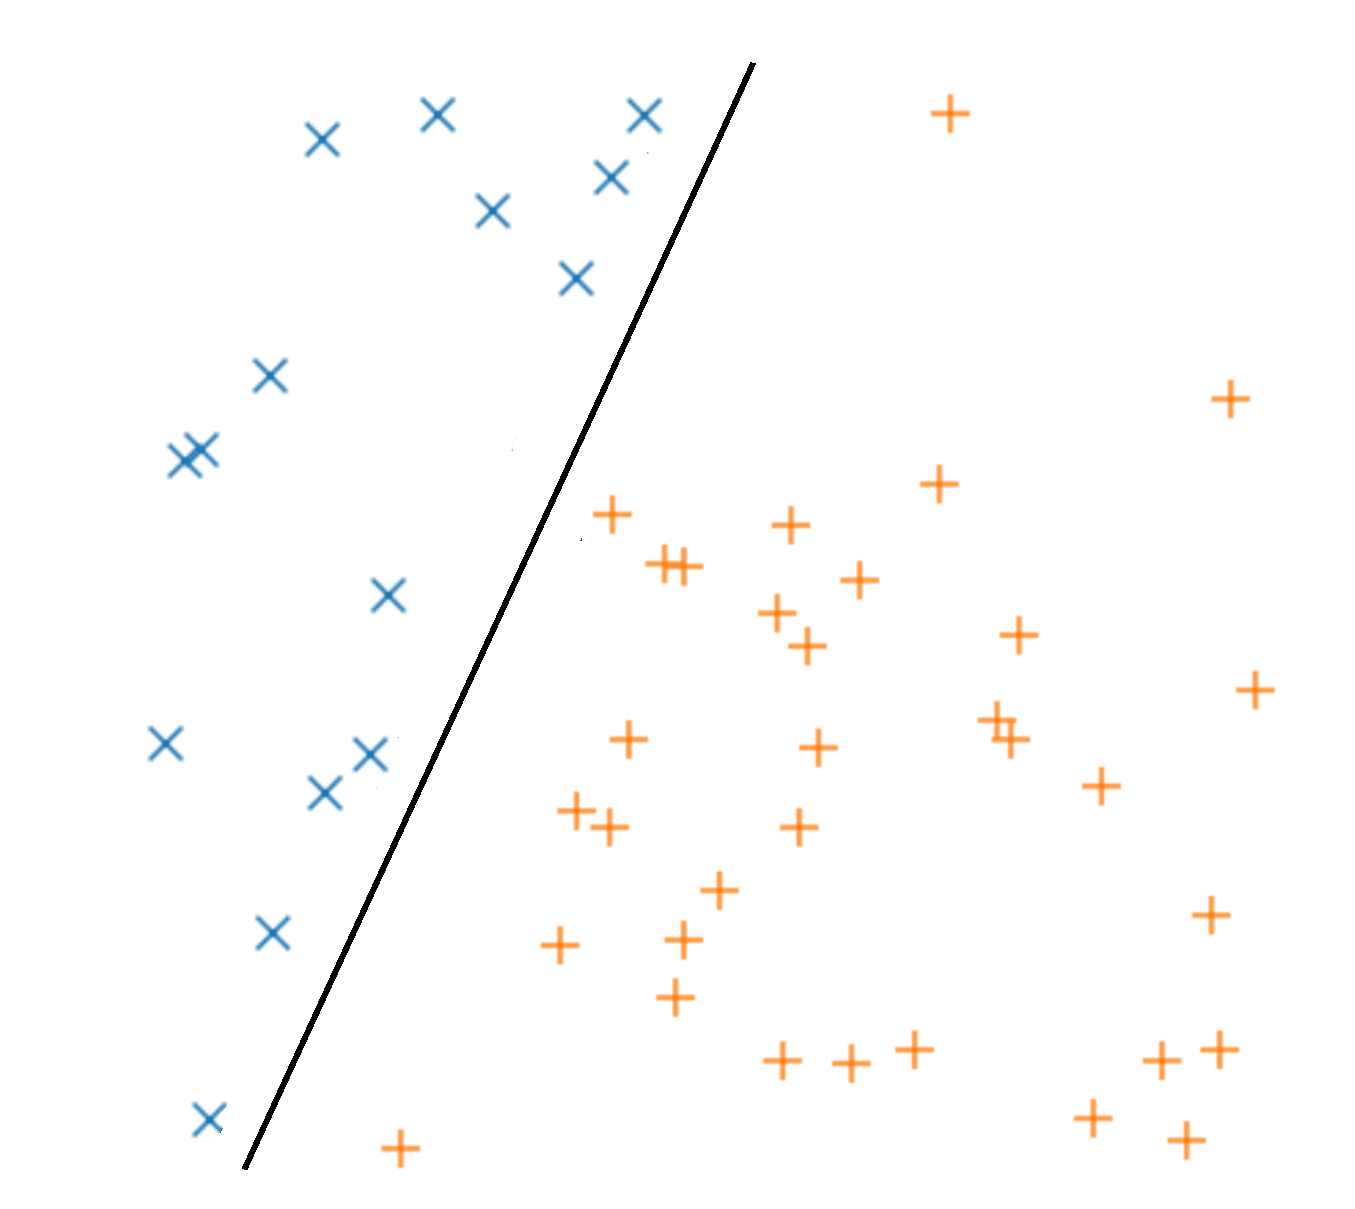
\includegraphics[width=1\textwidth,clip]{separabledroite.pdf}};
%					\node (ref) [visible on=<2>] {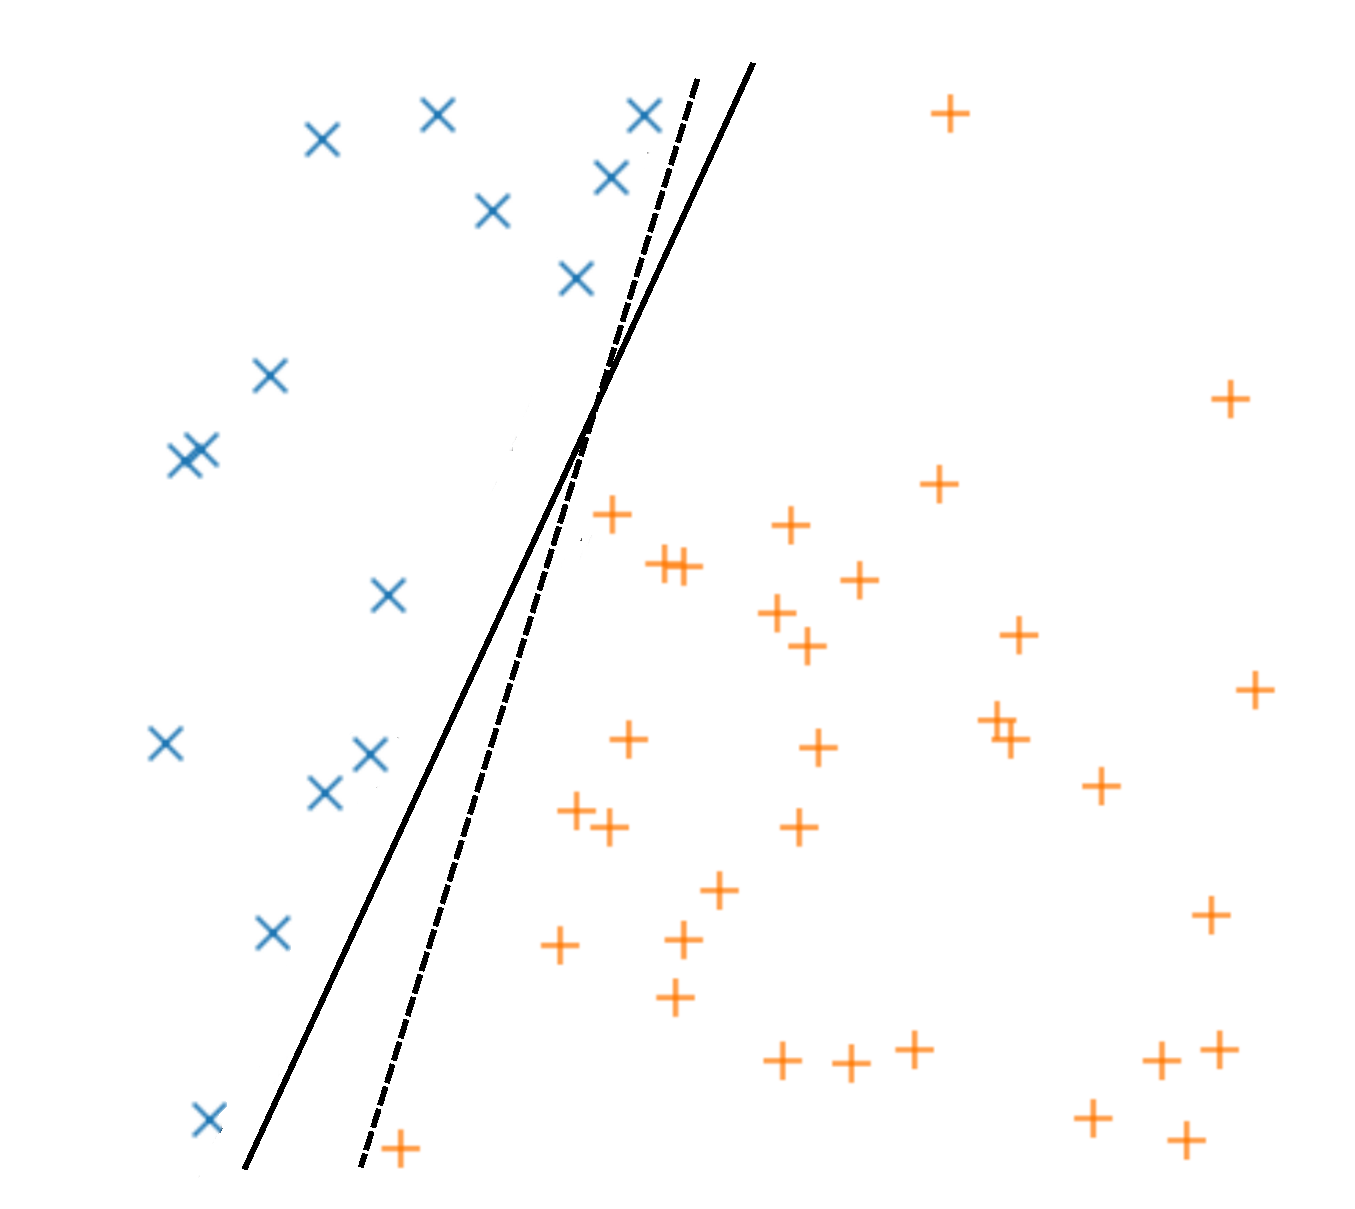
\includegraphics[width=1\textwidth,clip]{separabledroite1.pdf}};
%						\node (ref) [visible on=<3>] {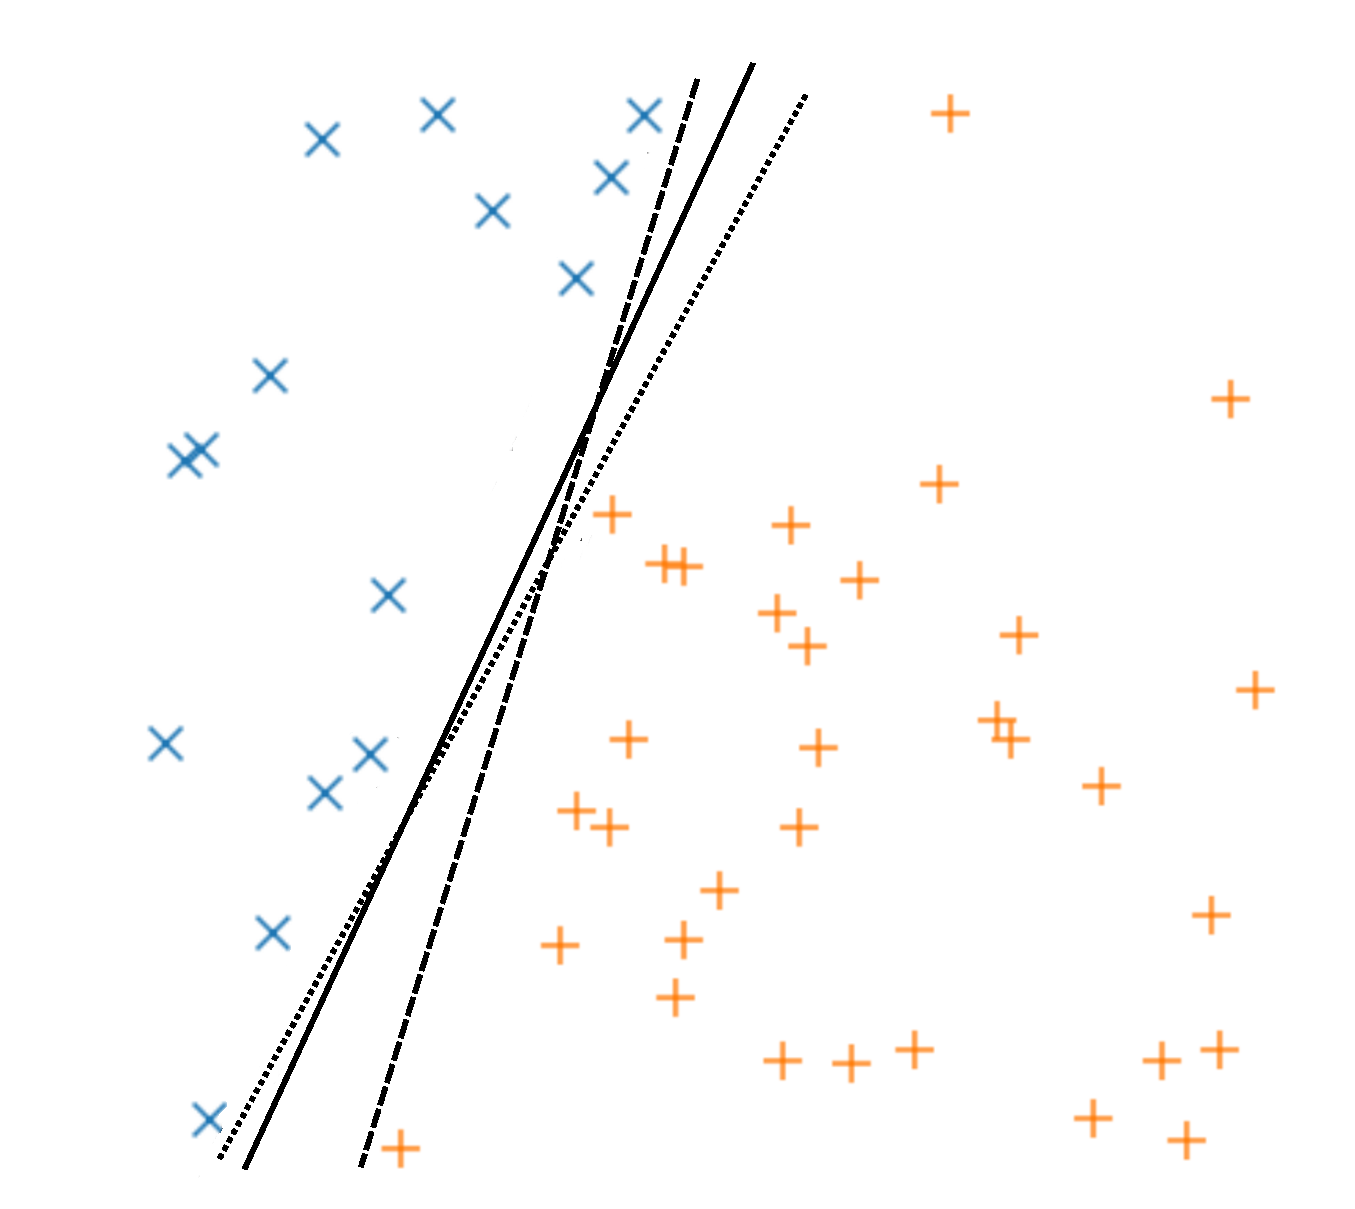
\includegraphics[width=1\textwidth,clip]{separabledroite2.pdf}};
%							\node (ref) [visible on=<4>] {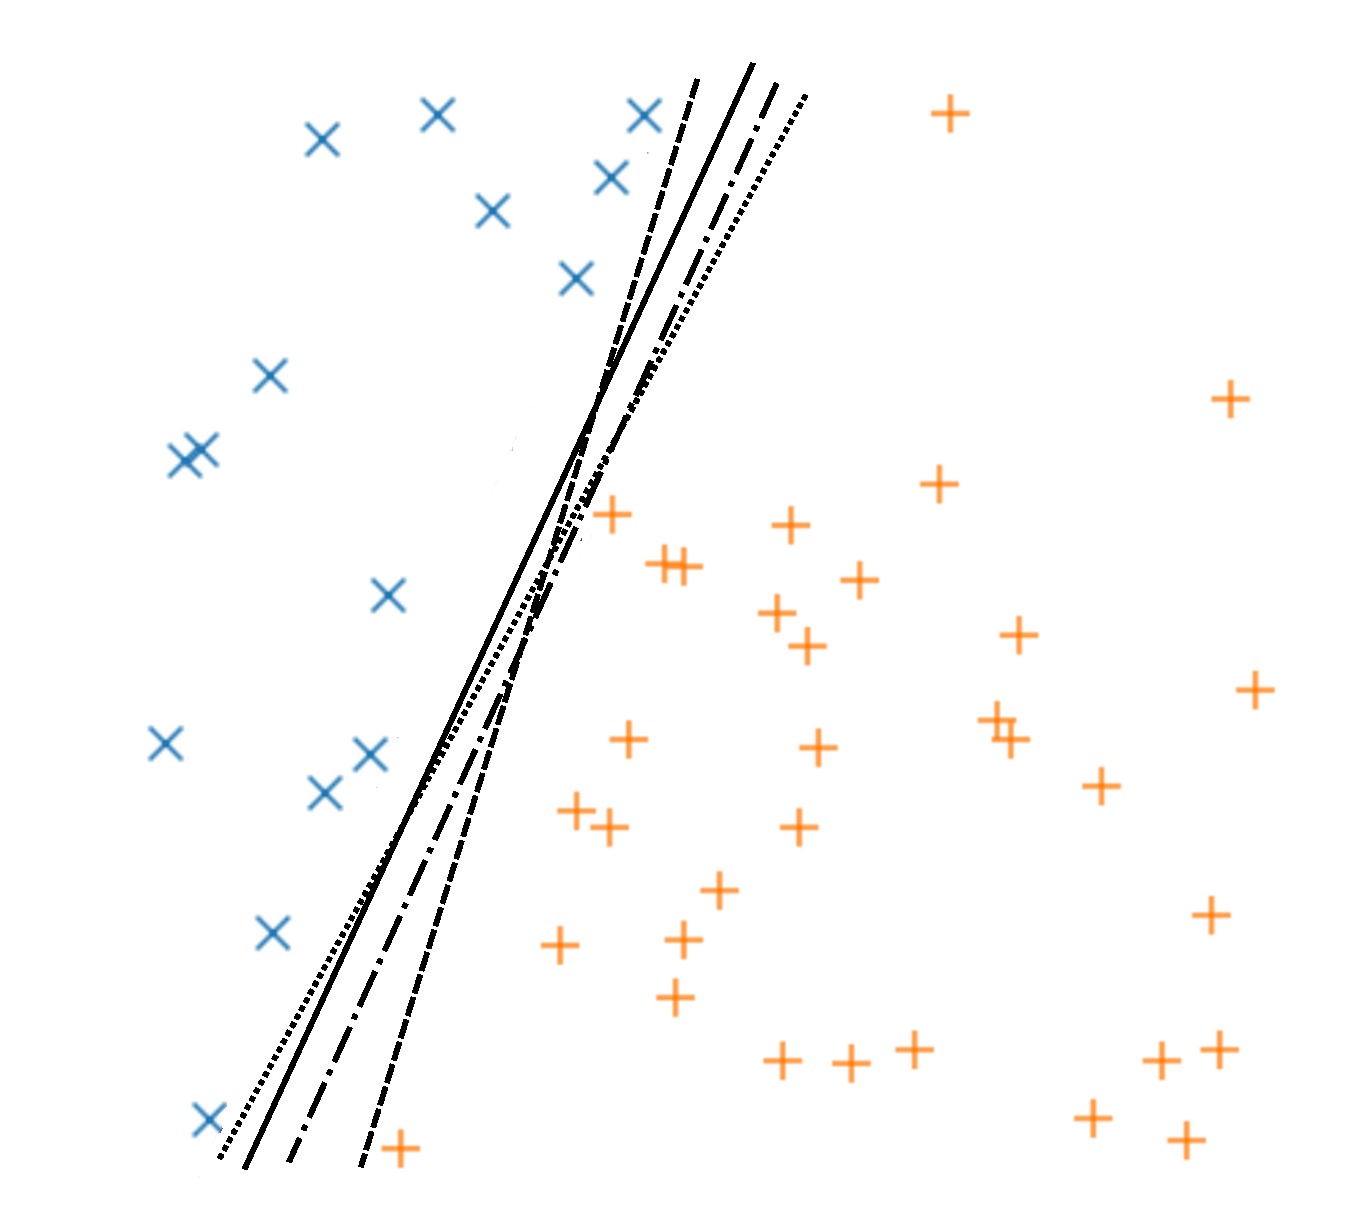
\includegraphics[width=1\textwidth,clip]{separabledroite3.pdf}};
%														\node (ref) [visible on=<5->] {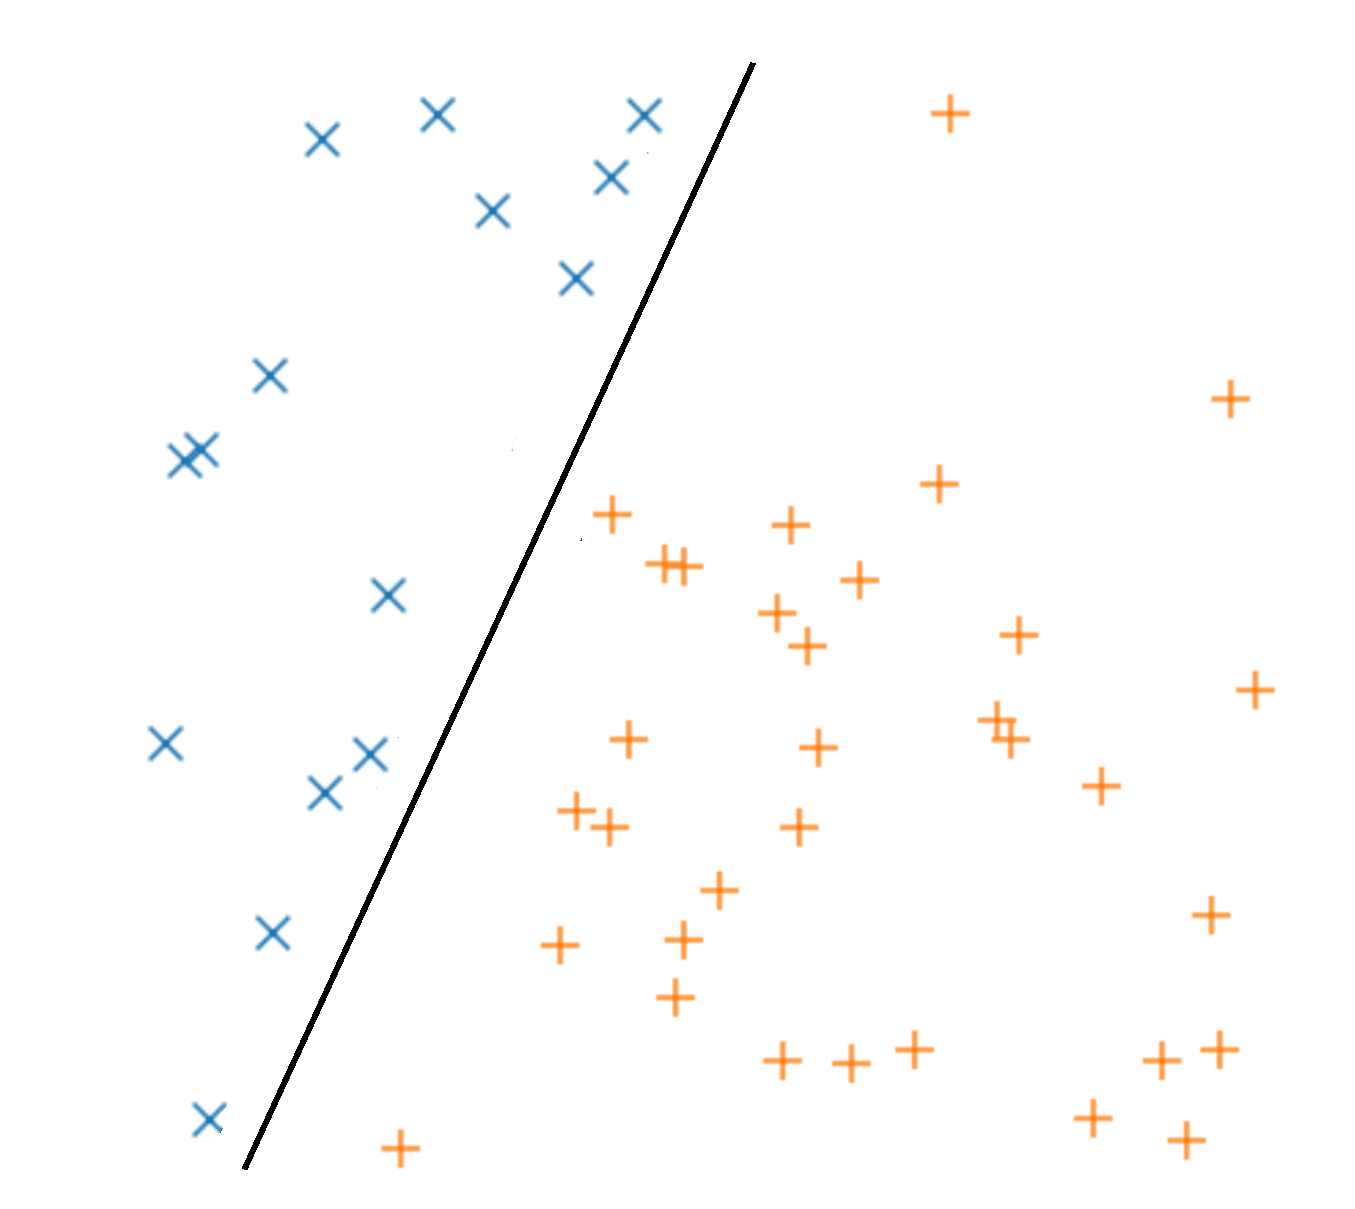
\includegraphics[width=1\textwidth,clip]{separabledroite.pdf}};
%		\end{tikzpicture}
%	\end{minipt}
%	\hfill
%	\begin{minipt}[0.48]{0.75}
%		
%			\vspace*{-14.9em}
%			Un hyperplan séparateur ne fait aucune erreur de classification sur les données d'apprentissage\\%: 			
%		%	$$ \dfrac{1}{n} \sum_{i=1}^n  $$
%			%
%			\vspace*{0.5em}
%			
%				\uncover<4->{
%				\begin{minipc}[0.13]{0.15}
%					\warning
%				\end{minipc}
%				\begin{minipc}[0.82]{0.15}
%				Il existe une infinité d'hyperplans séparateurs
%				\end{minipc}
%			}
%			
%			\vspace{1em}
%			\uncover<5->{
%				\begin{minipc}[0.13]{0.15}
%					\raisebox{1.5mm}{\bclampe \xspace} 
%				\end{minipc}
%				\begin{minipc}[0.75]{0.15}
%				L'hyperplan équidistant des observations positive et négative les plus proches semble préférable
%				\end{minipc}
%			}
%			
%		
%	\end{minipt}	
%	%------------------------NOTE
%\note{On idée pour savoir comment on choisit l'hyperplan}
%
%\end{frame}

%------------------------------------------------------------------------------------------
%------------------------------------------------------------------------------------------
\begin{frame}{Marges et vecteurs de support}
	%	\begin{minipt}[1]{0.37}
				\only<1-10>{
	\begin{minipc}[1]{0.37}
		\only<1-9>{
		\begin{minipt}[1]{0.2}	
		\textcolor{MPTblue}{\large\textbf{Définition}}	
	\begin{vblock}{}
\only<1-7>{	La marge $\gamma$ d’un hyperplan séparateur est la distance de cet hyperplan à
	l’observation du jeu d’apprentissage la plus proche.}
\only<8-9>{On appelle \textbf{vecteurs de support} les points $x_i$ du jeu d'apprentissage situés à une distance $\gamma$ de l’hyperplan séparateur $H$. Ils \textit{soutiennent} les hyperplans $H_+$ et $H_{-}$ situés à une distance $\gamma$ de $H$ }
	\end{vblock}
\end{minipt}
%	\vspace*{0.1em}
\begin{minipt}[1]{0.16}	
\only<1-7>{	
%\vspace*{0.3em}	
%\bftitle{Objectif} \hsp Chercher l'hyperplan séparateur équidistant des observations positive\\ \phantom{\bftitle{Objectif} \hsp}et négative les plus proches \ie \textbf{qui maximise sa marge} $\boldsymbol{\gamma}$ 
%\bftitle{Objectif} \hsp Chercher l'hyperplan séparateur qui est à une distance $\gamma$ d'au moins\\\phantom{\bftitle{Objectif} \hsp}une observation négative et une observation positive \ie chercher\\\phantom{\bftitle{Objectif} \hsp}l'hyperplan \textbf{qui maximise sa marge} $\boldsymbol{\gamma}$ 
%\uncover<1->{ \ie\\ \phantom{\bftitle{Objectif} \hsp}l'hyperplan pour lequel il y a au moins une observation négative et\\ \phantom{\bftitle{Objectif} \hsp}une observation positive qui sont à une distance $\gamma$ de cet hyperplan}

	\begin{minipage}[c][1.2cm][t]{0.13\textwidth}
		\bftitle{Objectif}
		\end{minipage}
	\begin{minipage}[c][1.2cm][t]{0.86\textwidth}
	Chercher l'hyperplan séparateur \textbf{qui maximise sa marge} $\boldsymbol{\gamma}$ .  Cet hyperplan sera à une distance $\gamma$ d'au moins une observation négative et une observation positive
		\end{minipage} 

	
}


\only<8>{
	\vspace{0.9em}
	
	Un déplacement léger d'au moins un des vecteurs de support peut modifier l'hyperplan séparateur $H$ qui maximise $\gamma$. À l’inverse, $H$ ne change pas si l’on déplace légèrement une observation qui n’est pas vecteur de support}
\only<9>{
	\vspace{0.9em}
	Cependant, même si un des vecteurs de support est légèrement déplacé et que cela entraîne une modification de $H$, ce dernier sera toujours un hyperplan séparateur. La méthode est donc robuste à de légères perturbations des données d'apprentissage}   
\end{minipt}
}
\only<10>{	
	\begin{minipt}[1]{0.4}	
	%\phantom{aa}\\
	\textcolor{MPTblue}{\large\textbf{Définition}}	
	\begin{vblock}{}
		La zone située entre $H_+$ et $H_{-}$ est appelée \textbf{zone d’indécision} ; elle ne contient aucune observation
\end{vblock}

Maximiser la marge permet donc de minimiser l'incertitude sur la classe à attribuer à une nouvelle observation $x$ qui tombe près de l'hyperplan séparateur $H$
\end{minipt}}
%\vspace{-5em}
\end{minipc}
}
%\end{minipt}

\begin{minipt}[1]{0.53}	
			\begin{center}
					\begin{tikzpicture}
							\node (ref) [visible on=<1>] at (0,11) {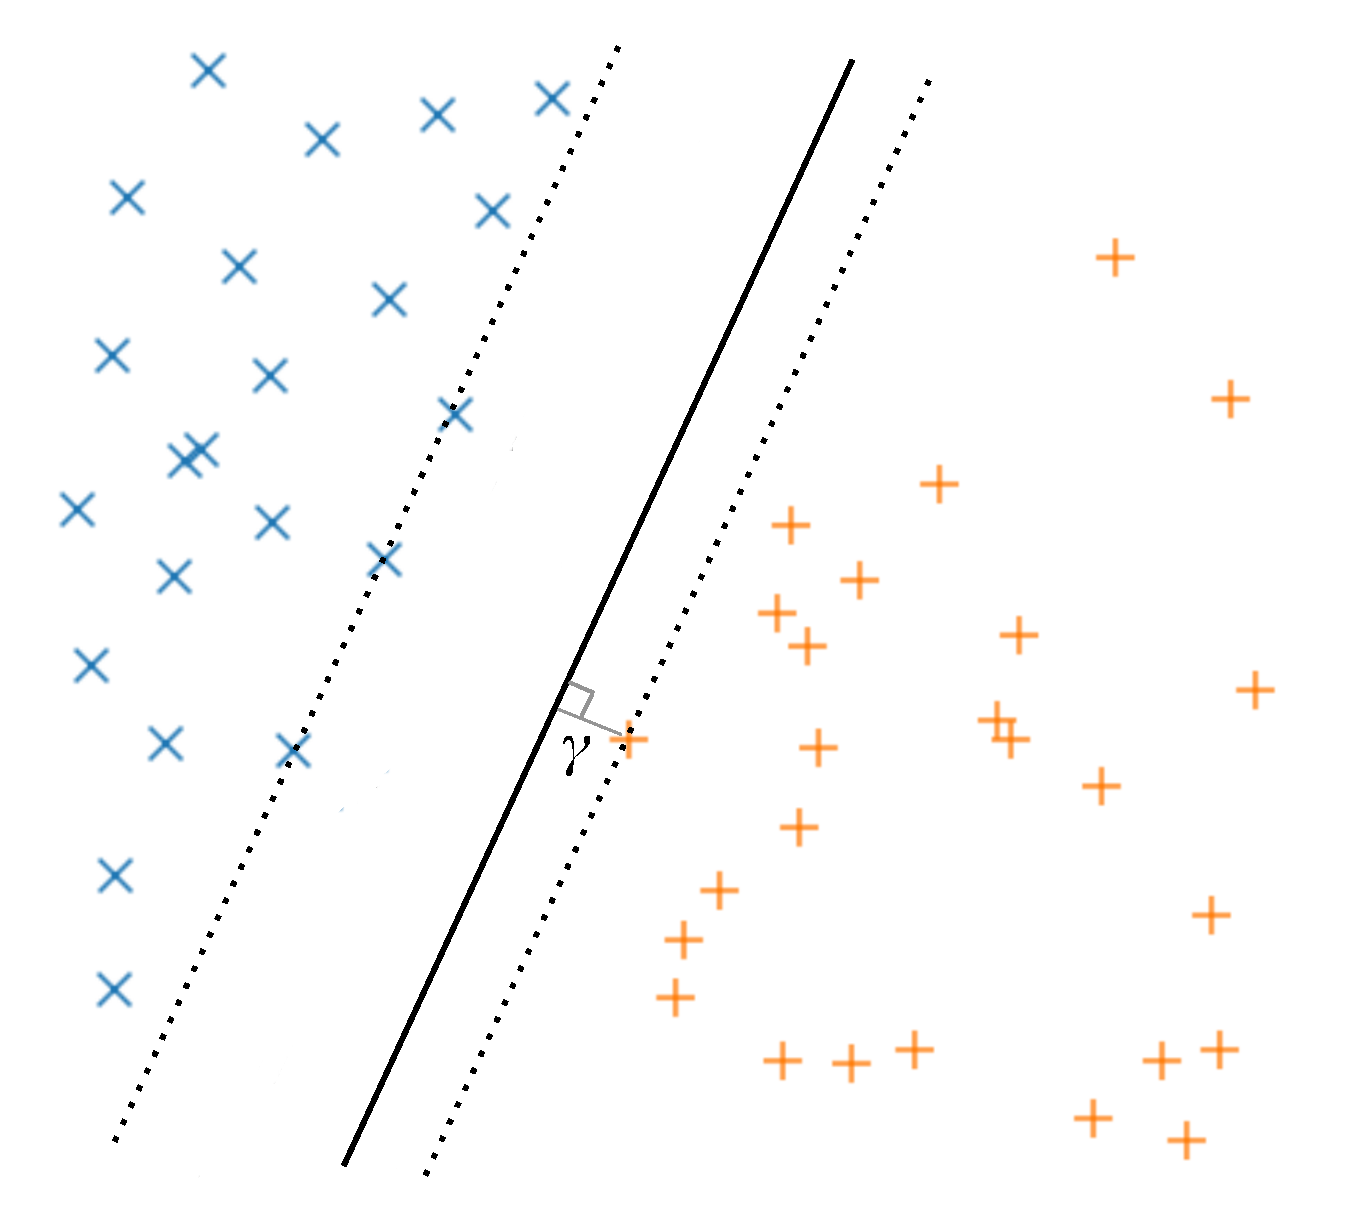
\includegraphics[width=0.43\textwidth,clip]{Images/marge1b.pdf}};
							\node (ref) [visible on=<2>] at (0,11) {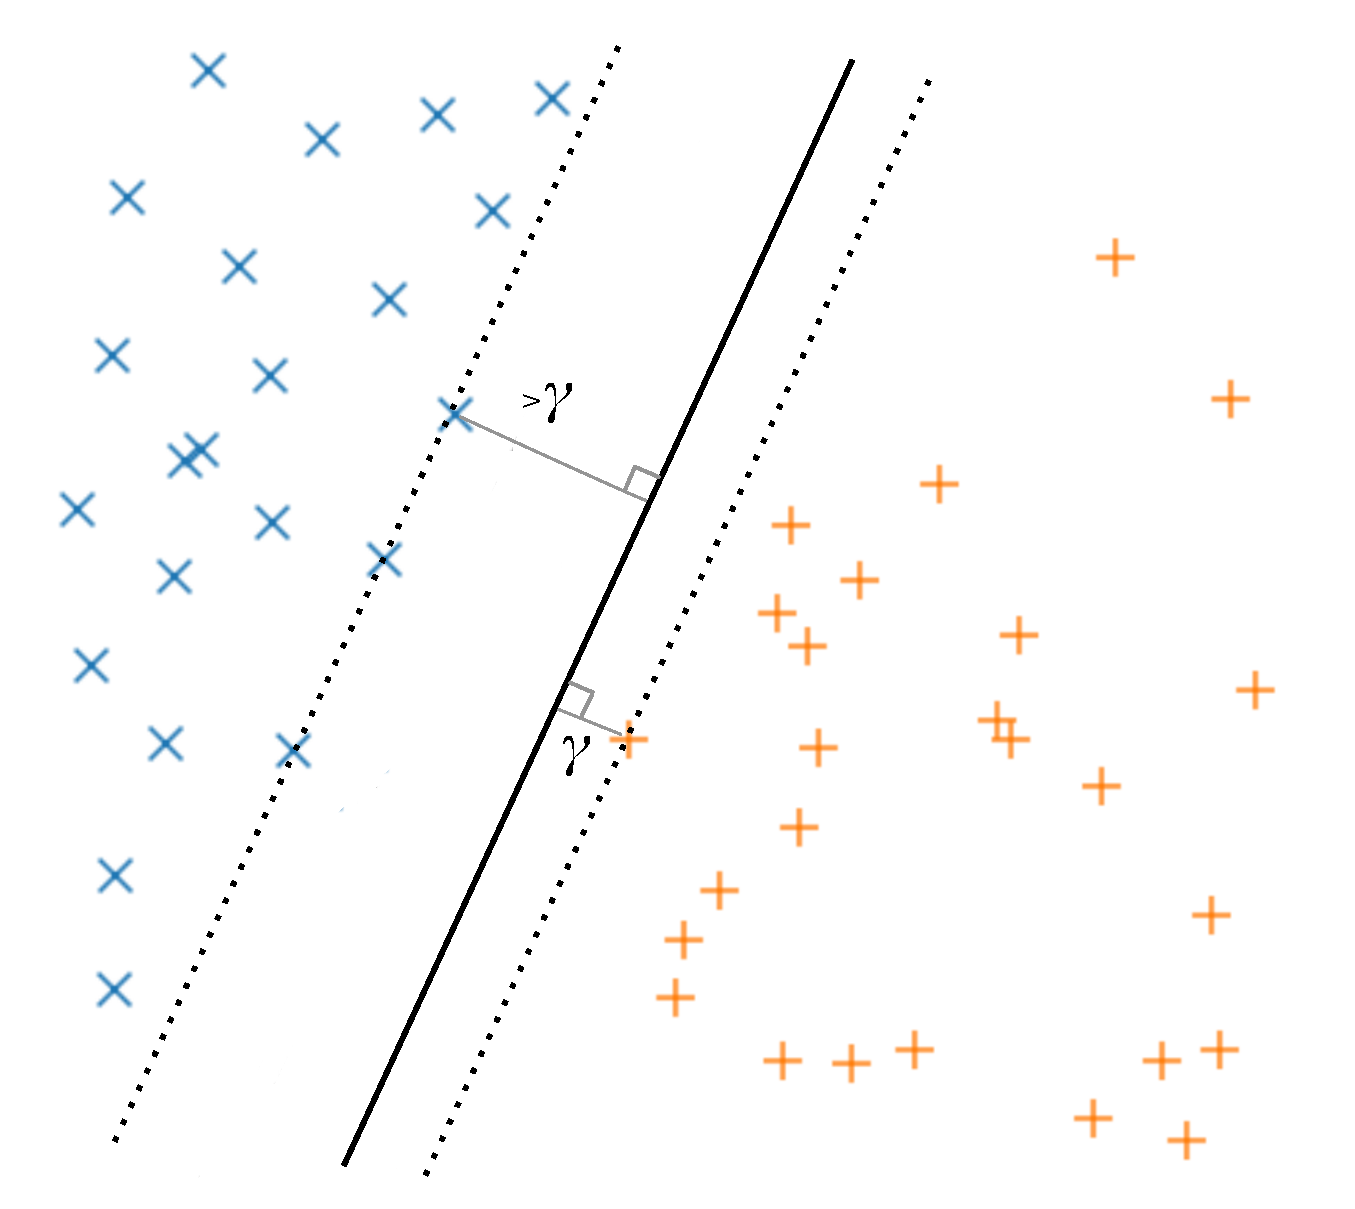
\includegraphics[width=0.43\textwidth,clip]{Images/marge2b.pdf}};
							\node (ref) [visible on=<3>] at (0,11) {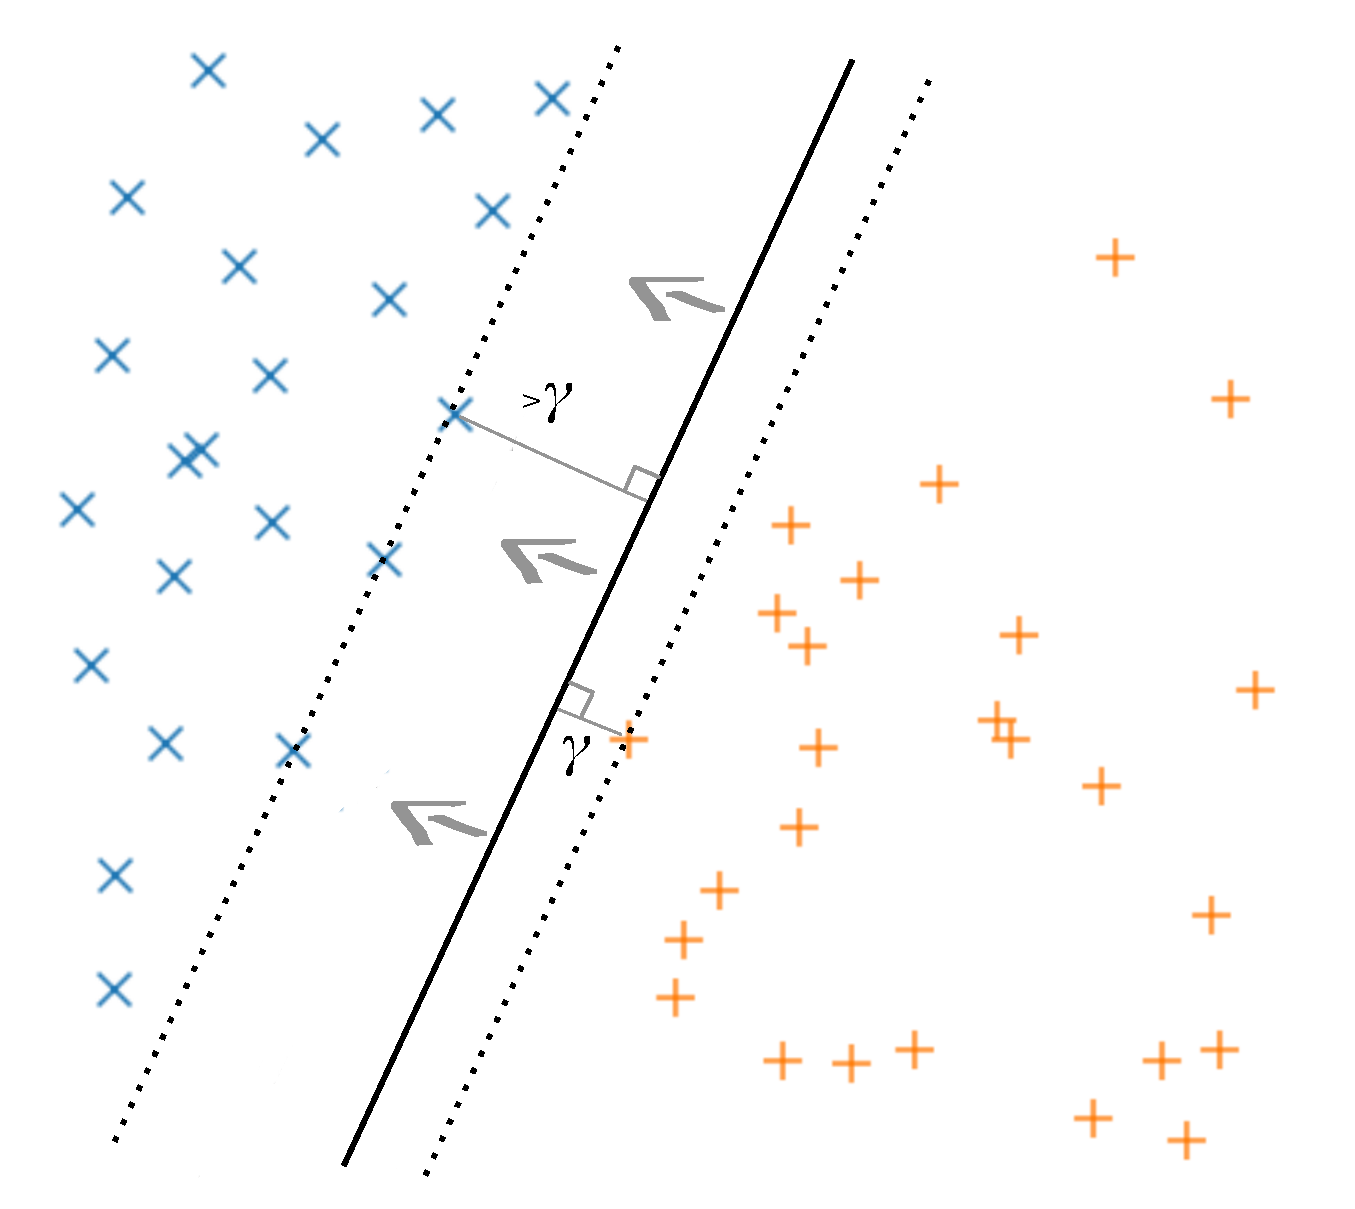
\includegraphics[width=0.43\textwidth,clip]{Images/marge3b.pdf}};
							\node (ref) [visible on=<4>] at (0,11) {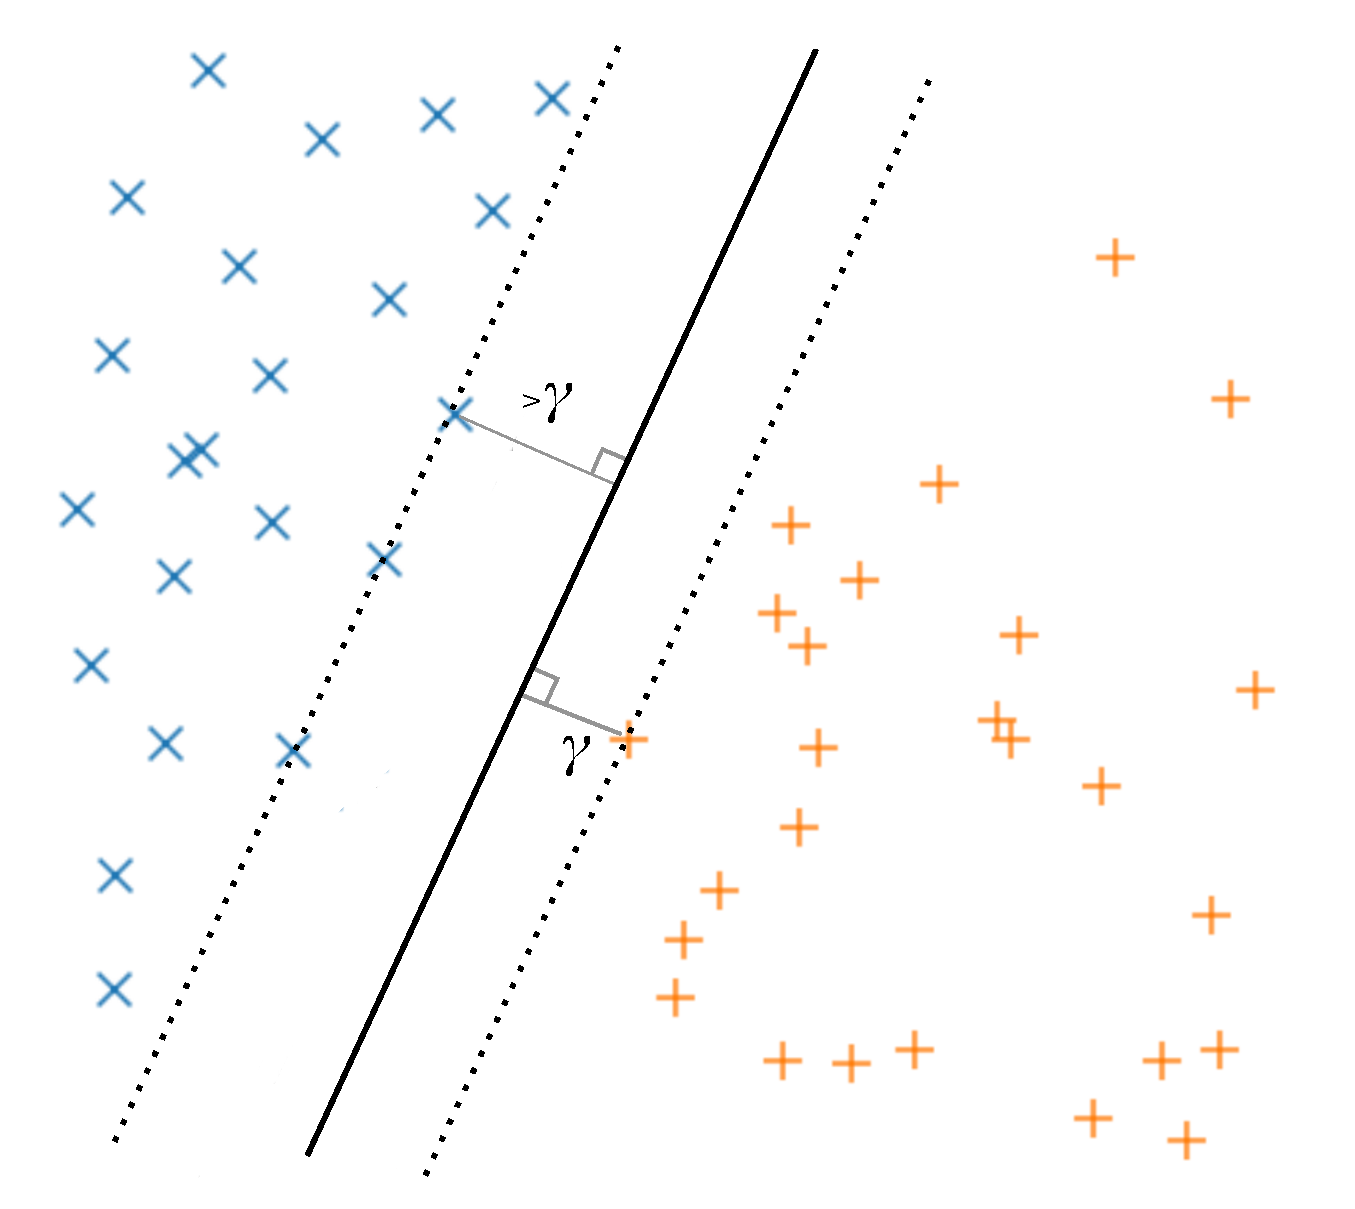
\includegraphics[width=0.43\textwidth,clip]{Images/marge4b.pdf}};
							\node (ref) [visible on=<5>] at (0,11) {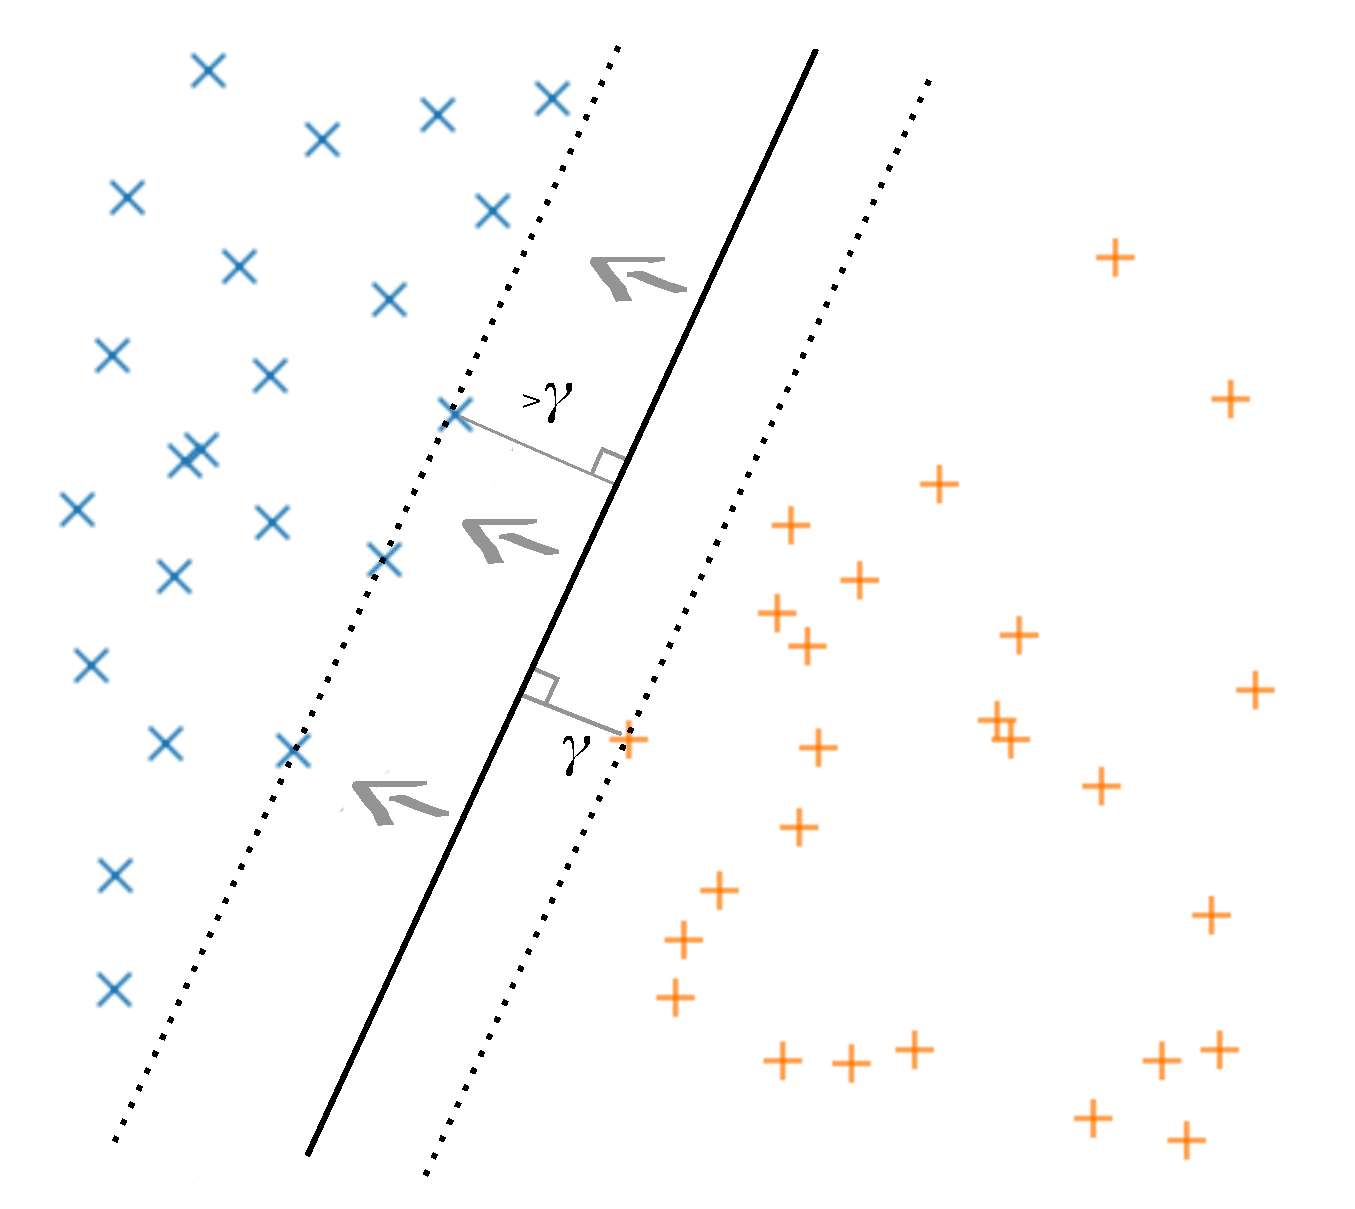
\includegraphics[width=0.43\textwidth,clip]{Images/marge5b.pdf}};
							\node (ref) [visible on=<6>] at (0,11) {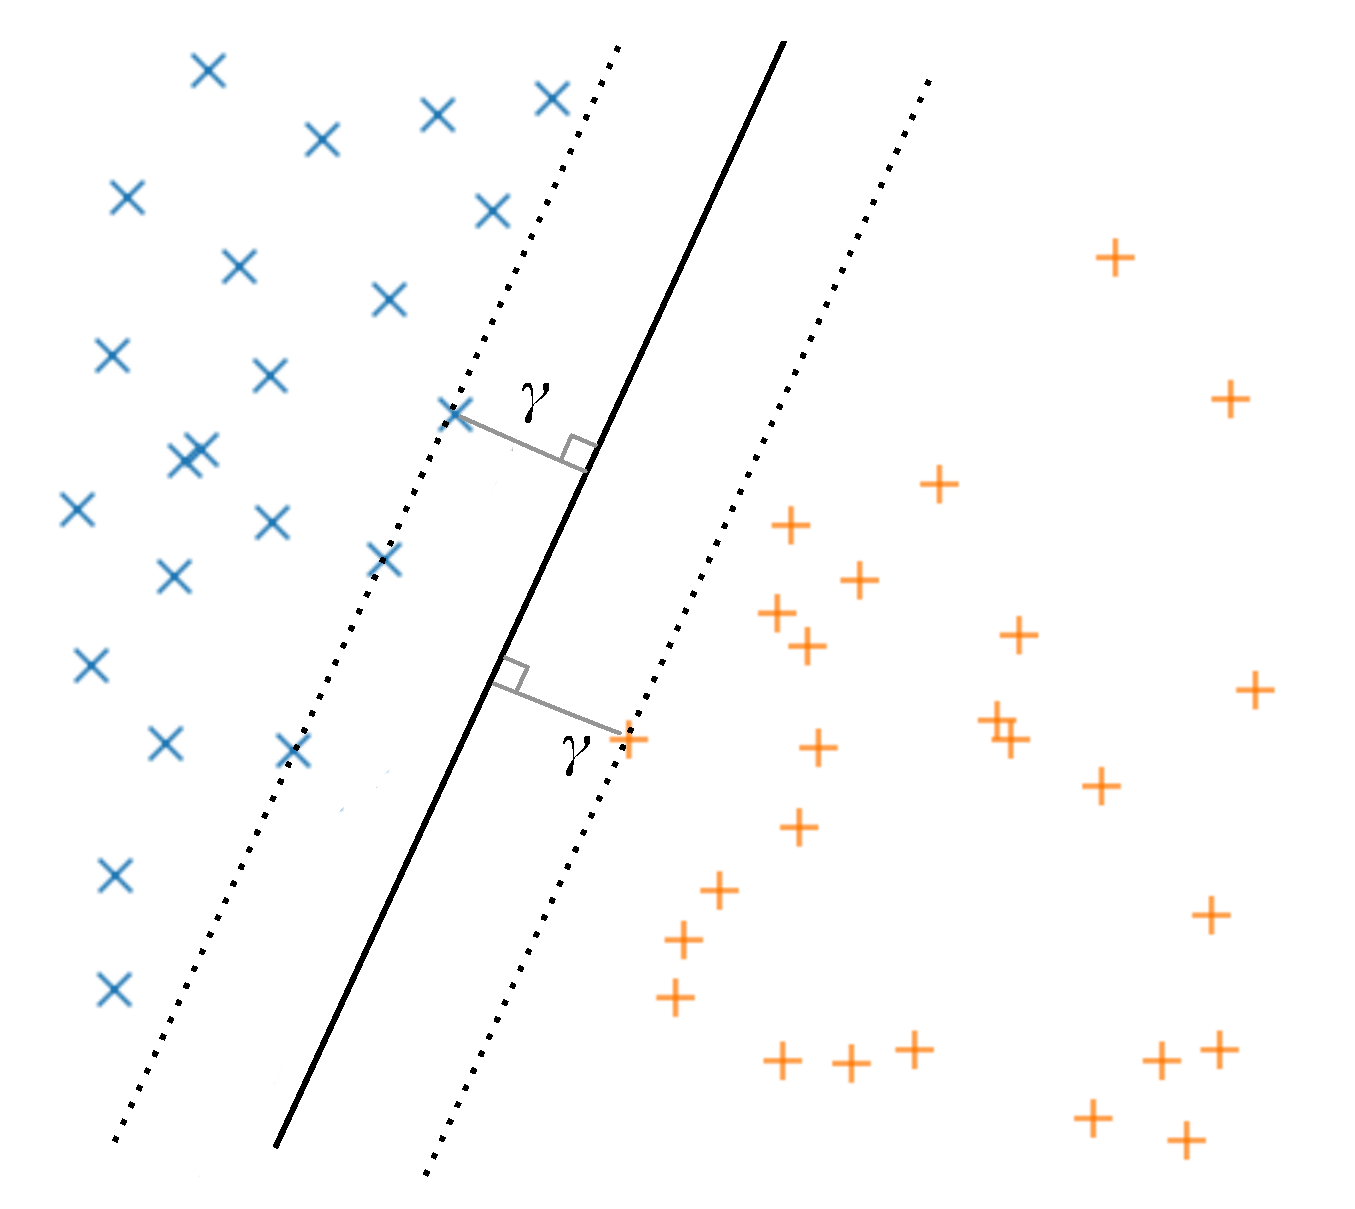
\includegraphics[width=0.43\textwidth,clip]{Images/marge6b.pdf}};
							\node (ref) [visible on=<7>] at (0,11) {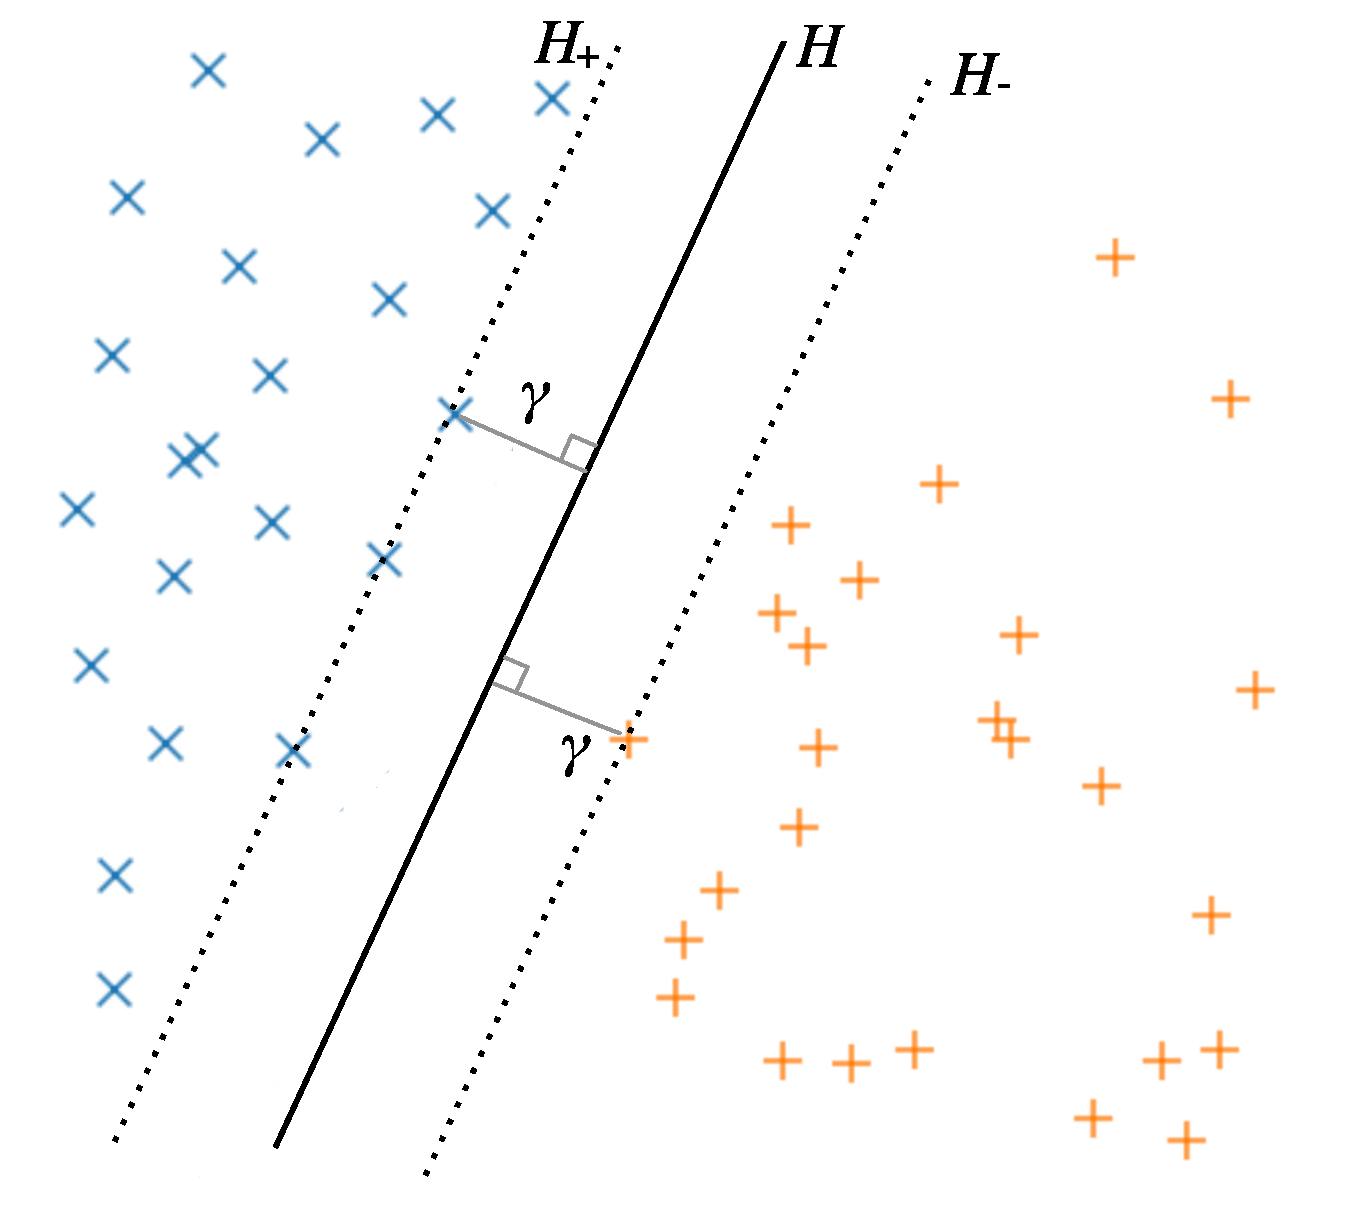
\includegraphics[width=0.43\textwidth,clip]{Images/marge7b.pdf}};
							\node (ref) [visible on=<8->] at (0,11) {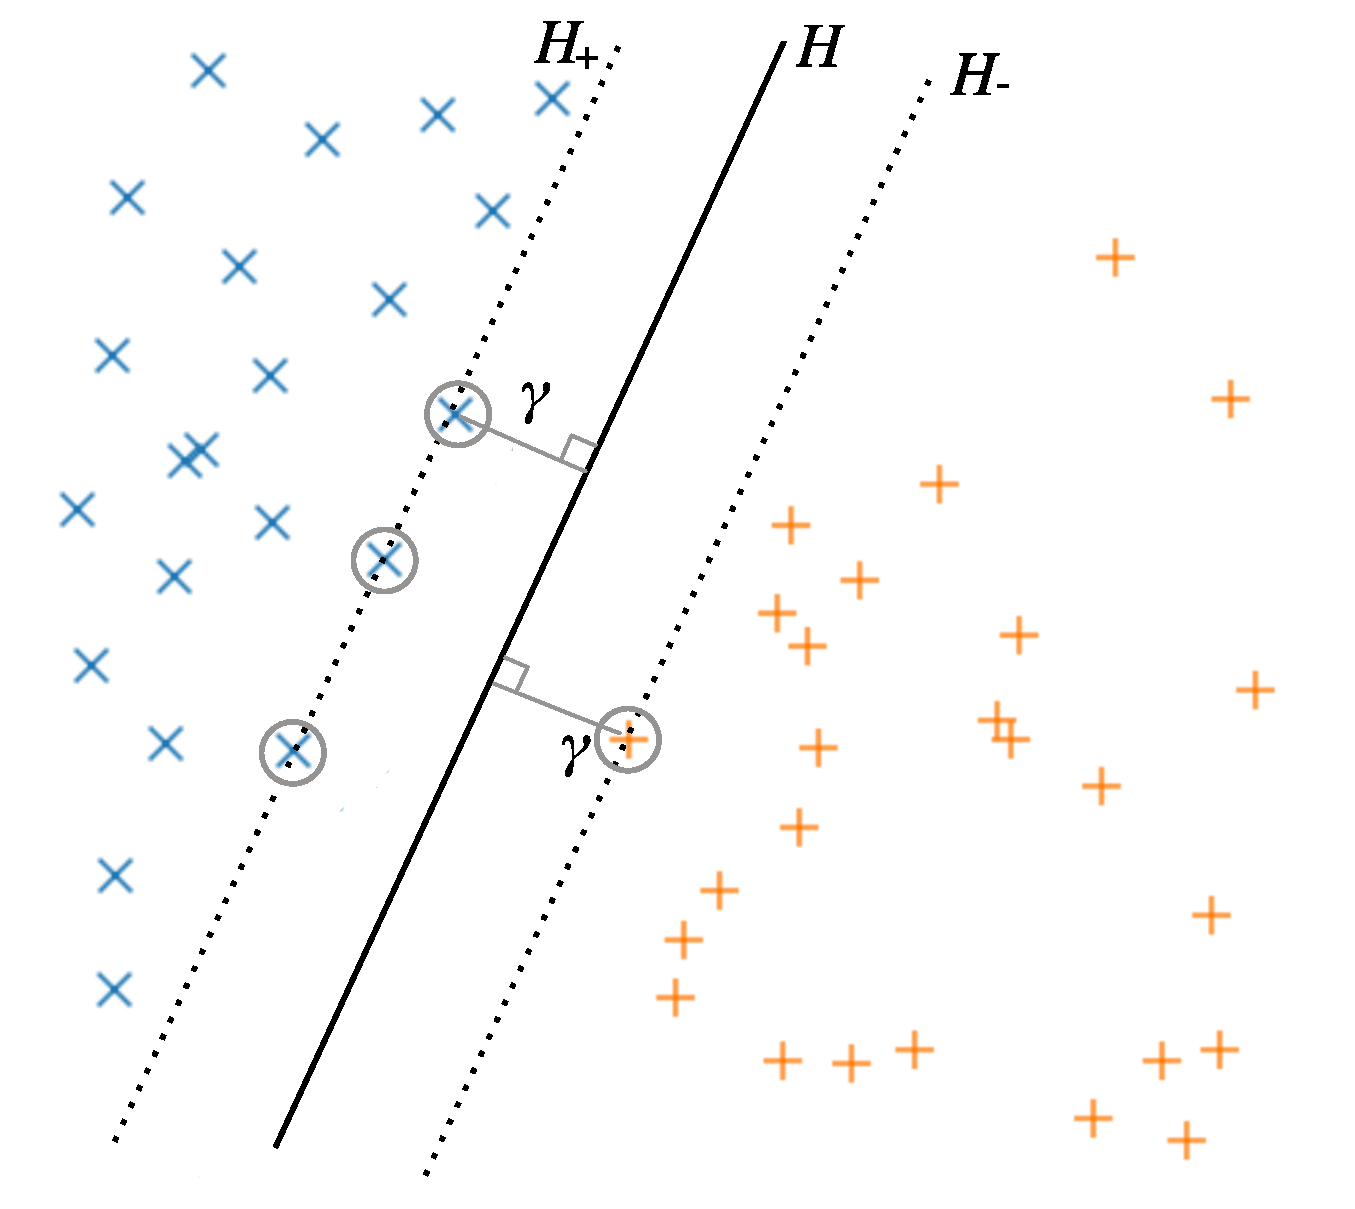
\includegraphics[width=0.43\textwidth,clip]{Images/marge8b.pdf}};
						\end{tikzpicture}
				\end{center}

\end{minipt}


%---------------Note
\note{dire que plus un point est proche de l'hyperplan, plus on a d'incertitude donc on voudraient qu'ils soient tous éloignés le plus possible}
\end{frame}


%\begin{frame}{Marges et vecteurs supports}
%	\only<1-7>{
%	\begin{minipt}[1]{0.36}
%			\textcolor{MPTblue}{\large\textbf{Définition}}	
%				\begin{vblock}{}
%					\only<1-6>{	La marge $\gamma$ d’un hyperplan séparateur est la distance de cet hyperplan à
%						l’observation du jeu d’apprentissage la plus proche.}
%					\only<7>{On appelle \textbf{vecteurs de support} les points $x_i$ du jeu d'apprentissage situées à une distance $\gamma$ de l’hyperplan séparateur $H$. Ils \textit{soutiennent} $H_+$ et $H_{-}$}
%					\only<8>{La zone située entre $H_+$ et $H_{-}$ est appelée \textbf{zone d’indécision} ; elle ne contient aucune observation}
%			\end{vblock}
%			%	\vspace*{0.1em}
%				\only<1-6>{	
%					%\vspace*{0.3em}	
%					%\bftitle{Objectif} \hsp Chercher l'hyperplan séparateur équidistant des observations positive\\ \phantom{\bftitle{Objectif} \hsp}et négative les plus proches \ie \textbf{qui maximise sa marge} $\boldsymbol{\gamma}$ 
%					\bftitle{Objectif} \hsp Chercher l'hyperplan séparateur qui est à une distance $\gamma$ d'au moins\\\phantom{\bftitle{Objectif} \hsp}une observation négative et une observation positive \ie chercher\\\phantom{\bftitle{Objectif} \hsp}l'hyperplan \textbf{qui maximise sa marge} $\boldsymbol{\gamma}$ 
%					%\uncover<1->{ \ie\\ \phantom{\bftitle{Objectif} \hsp}l'hyperplan pour lequel il y a au moins une observation négative et\\ \phantom{\bftitle{Objectif} \hsp}une observation positive qui sont à une distance $\gamma$ de cet hyperplan}
%				}
%				\only<7>{
%					Un déplacement léger d'au moins un des vecteurs de support peut modifier l'hyperplan séparateur $H$ qui maximise $\gamma$. À l’inverse, $H$ ne change pas si l’on déplace légèrement une observation qui n’est pas vecteur de support}
%	\end{minipt}
%}
%\only<8>{
%	\begin{minipc}[1]{0.36}
%		\phantom{Un déplacement léger d'au moins un des vecteurs de support peut modifier l'hyperplan séparateur $H$ qui maximise $\gamma$.}
%		\textcolor{MPTblue}{\large\textbf{Définition}}	
%		\begin{vblock}{}
%		La zone située entre $H_+$ et $H_{-}$ est appelée \textbf{zone d’indécision} ; elle ne contient aucune observation
%		\end{vblock}
%	\end{minipc}
%}	
%	
%	\begin{minipt}[1]{0.54}	
%		\begin{center}
%			\begin{tikzpicture}
%				\node (ref) [visible on=<1>] at (0,11) {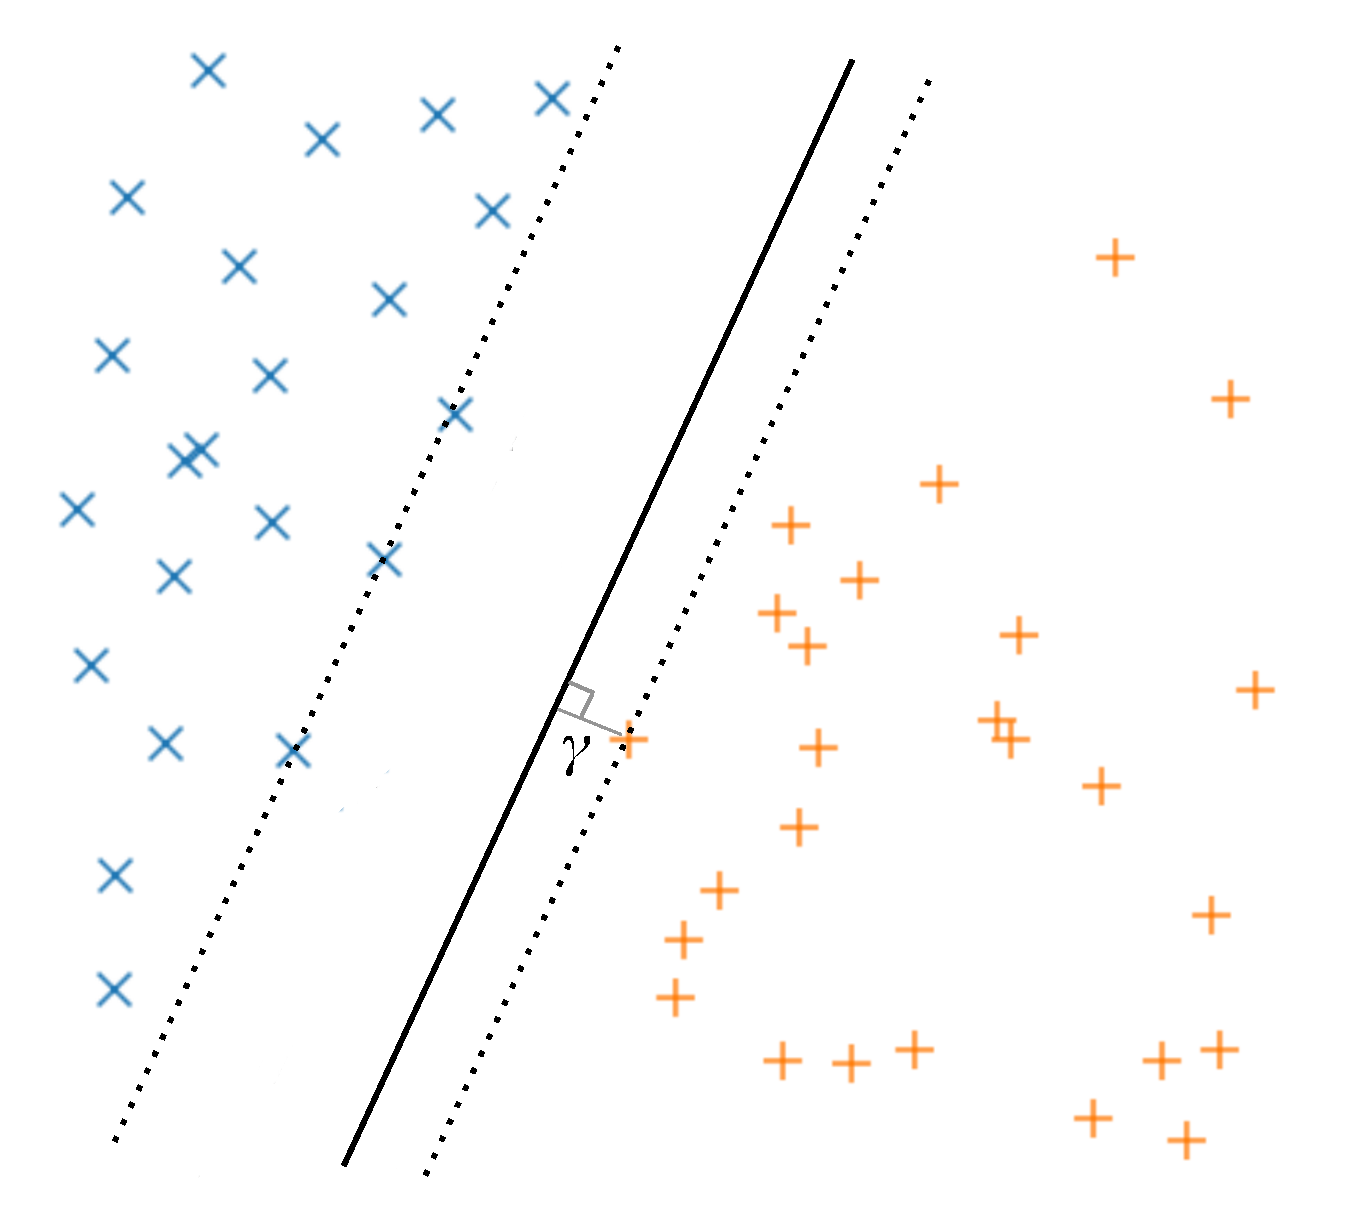
\includegraphics[width=0.43\textwidth,clip]{Images/marge1b.pdf}};
%				\node (ref) [visible on=<2>] at (0,11) {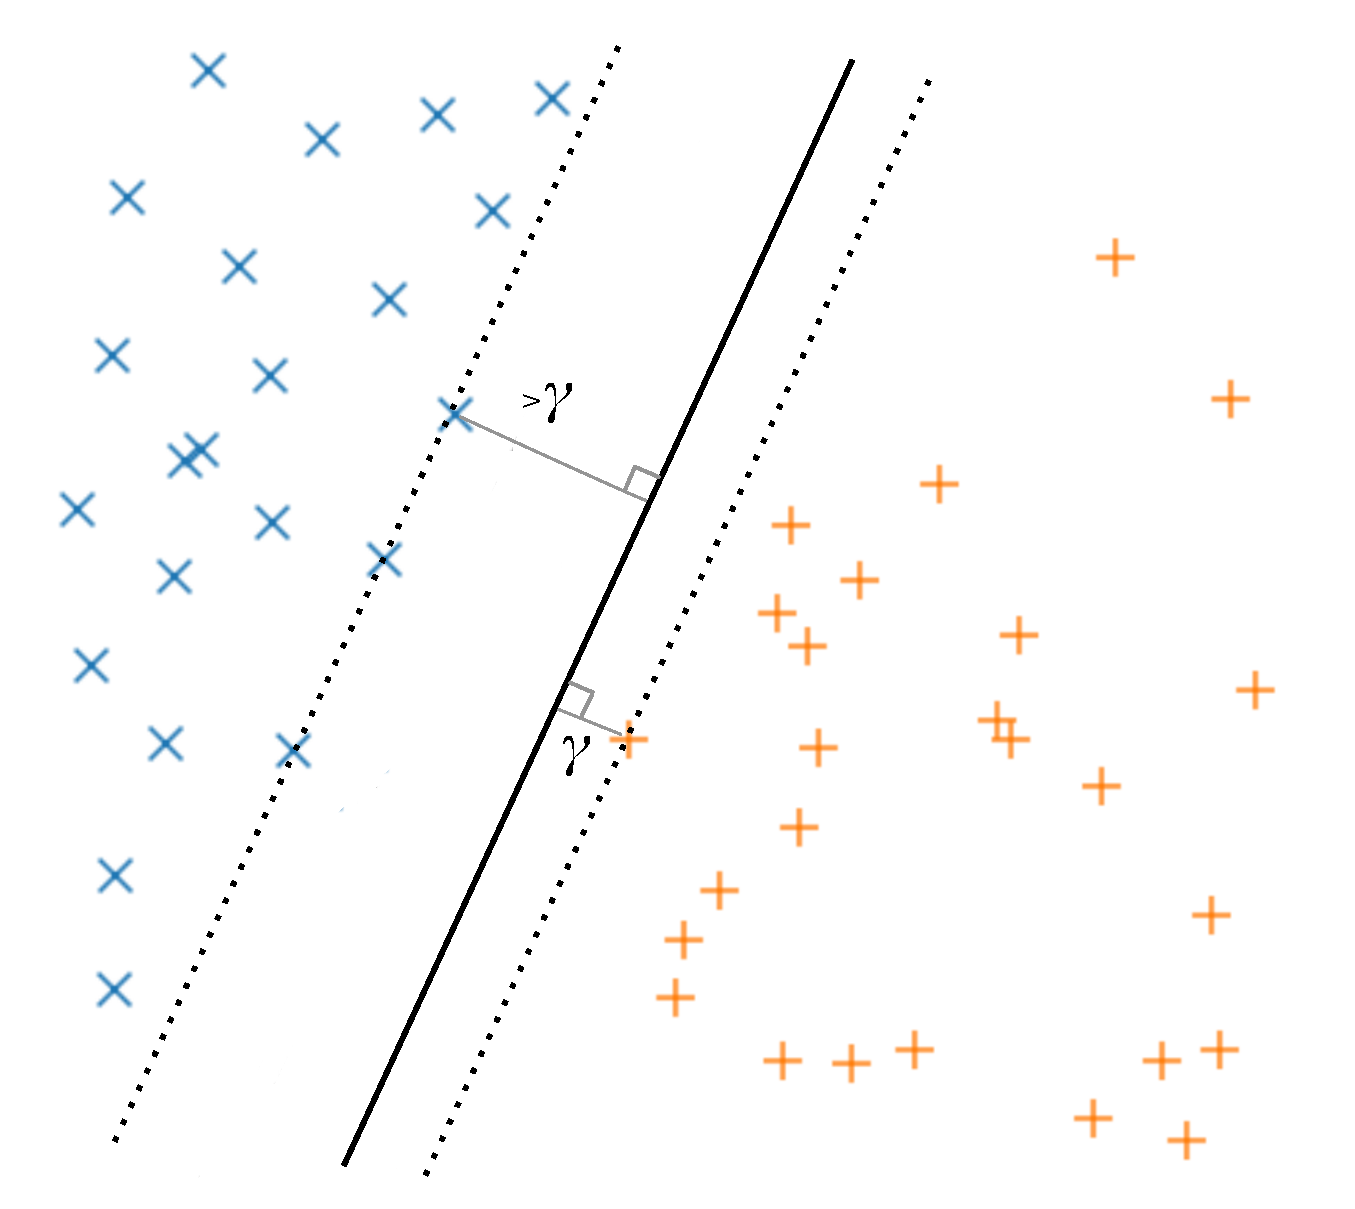
\includegraphics[width=0.43\textwidth,clip]{Images/marge2b.pdf}};
%				\node (ref) [visible on=<3>] at (0,11) {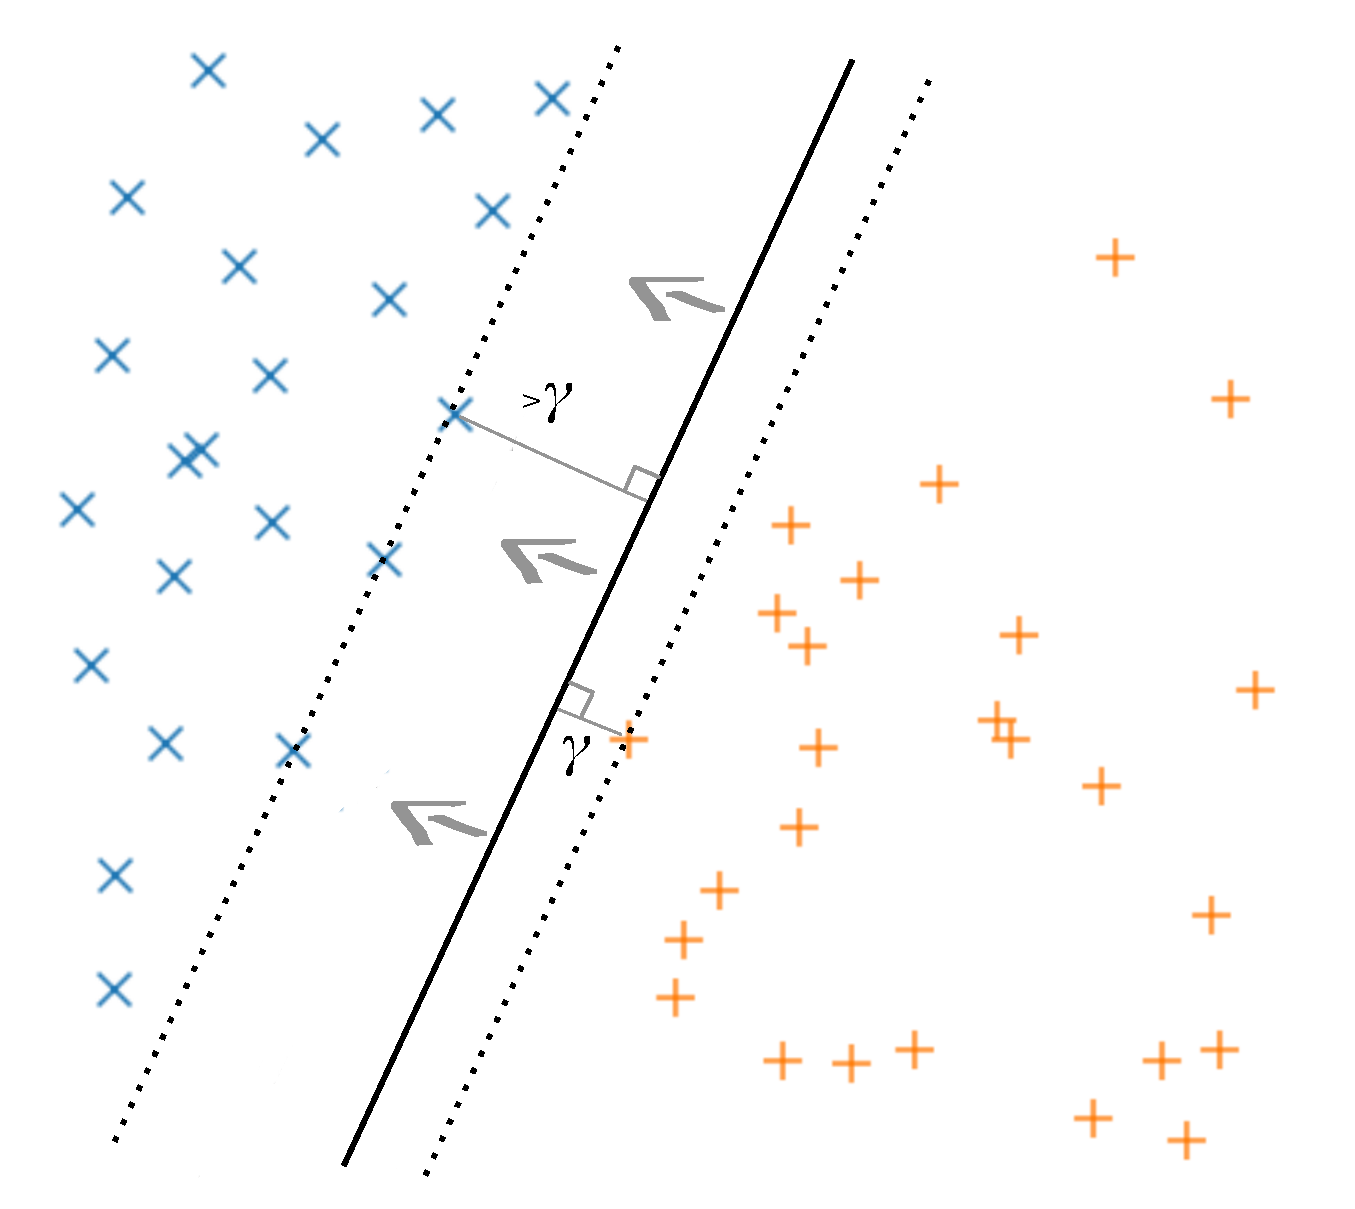
\includegraphics[width=0.43\textwidth,clip]{Images/marge3b.pdf}};
%				\node (ref) [visible on=<4>] at (0,11) {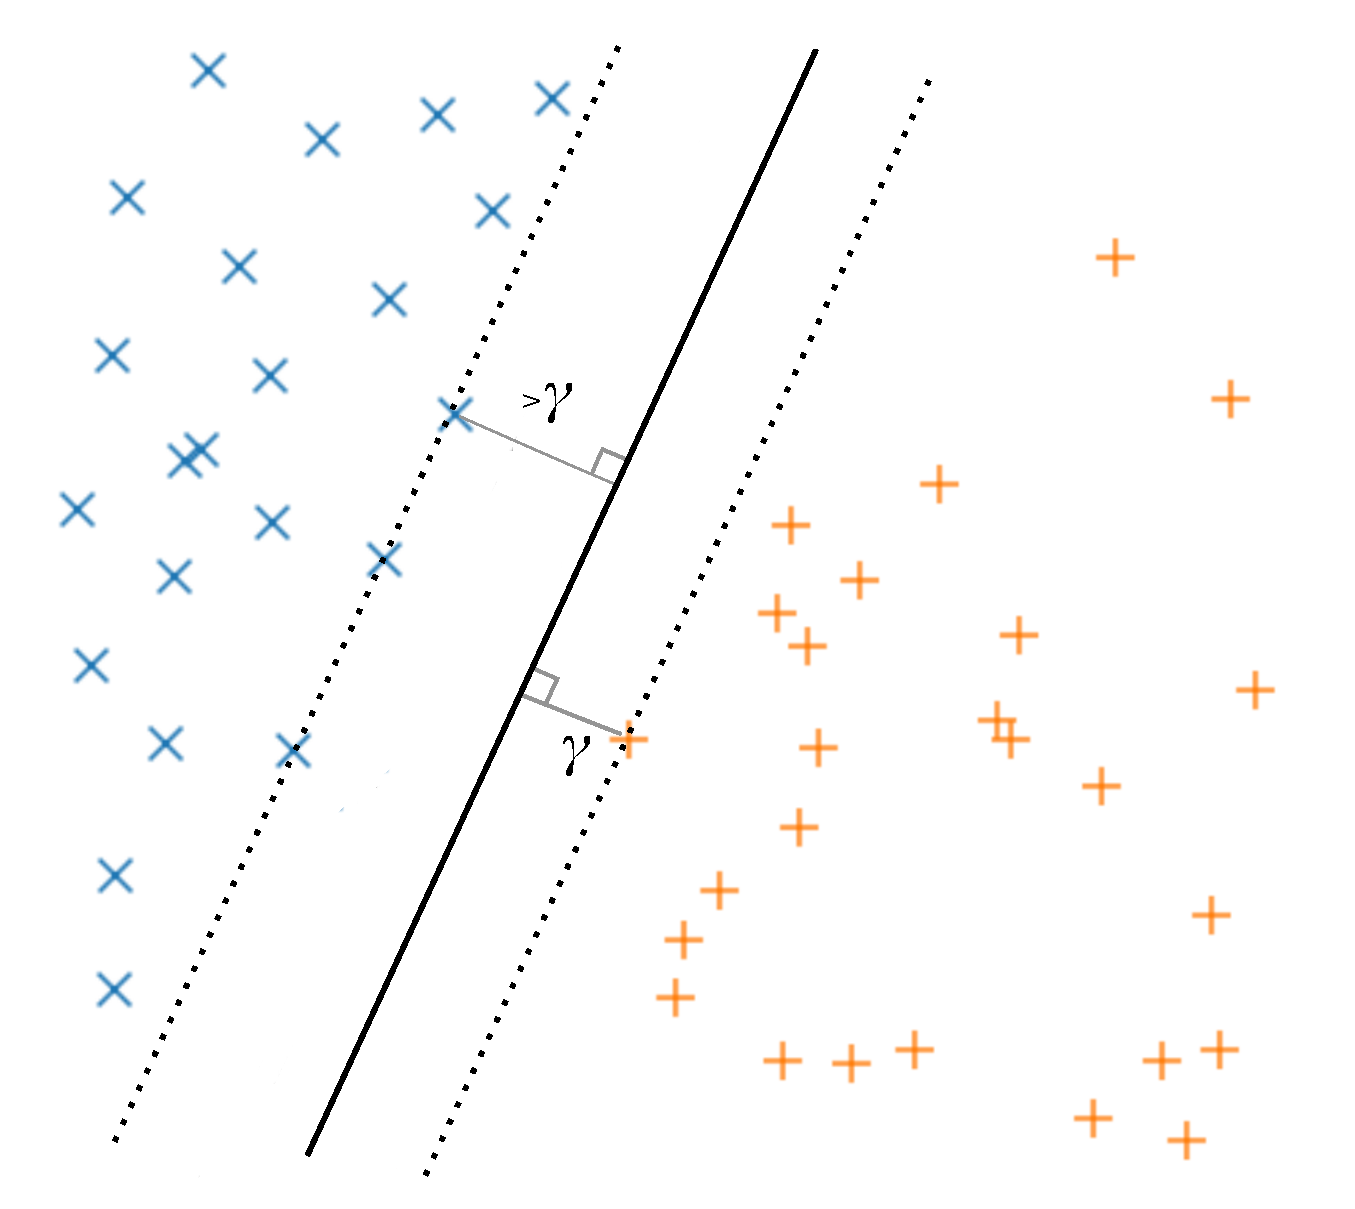
\includegraphics[width=0.43\textwidth,clip]{Images/marge4b.pdf}};
%				\node (ref) [visible on=<5>] at (0,11) {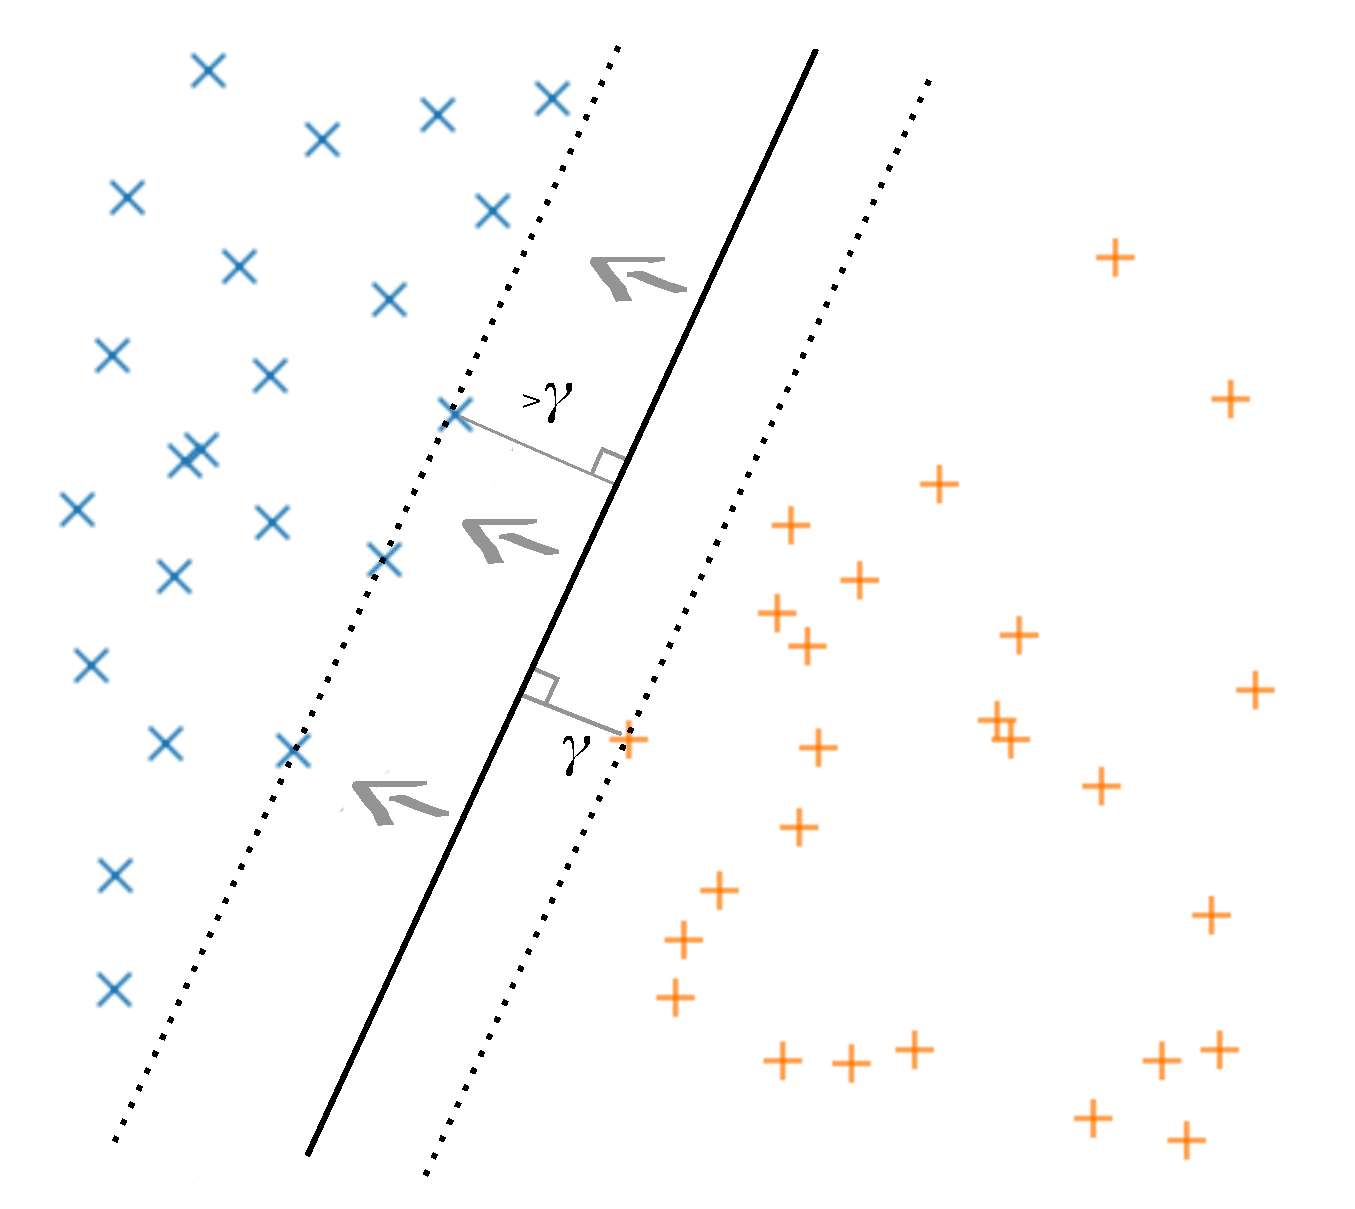
\includegraphics[width=0.43\textwidth,clip]{Images/marge5b.pdf}};
%				\node (ref) [visible on=<6>] at (0,11) {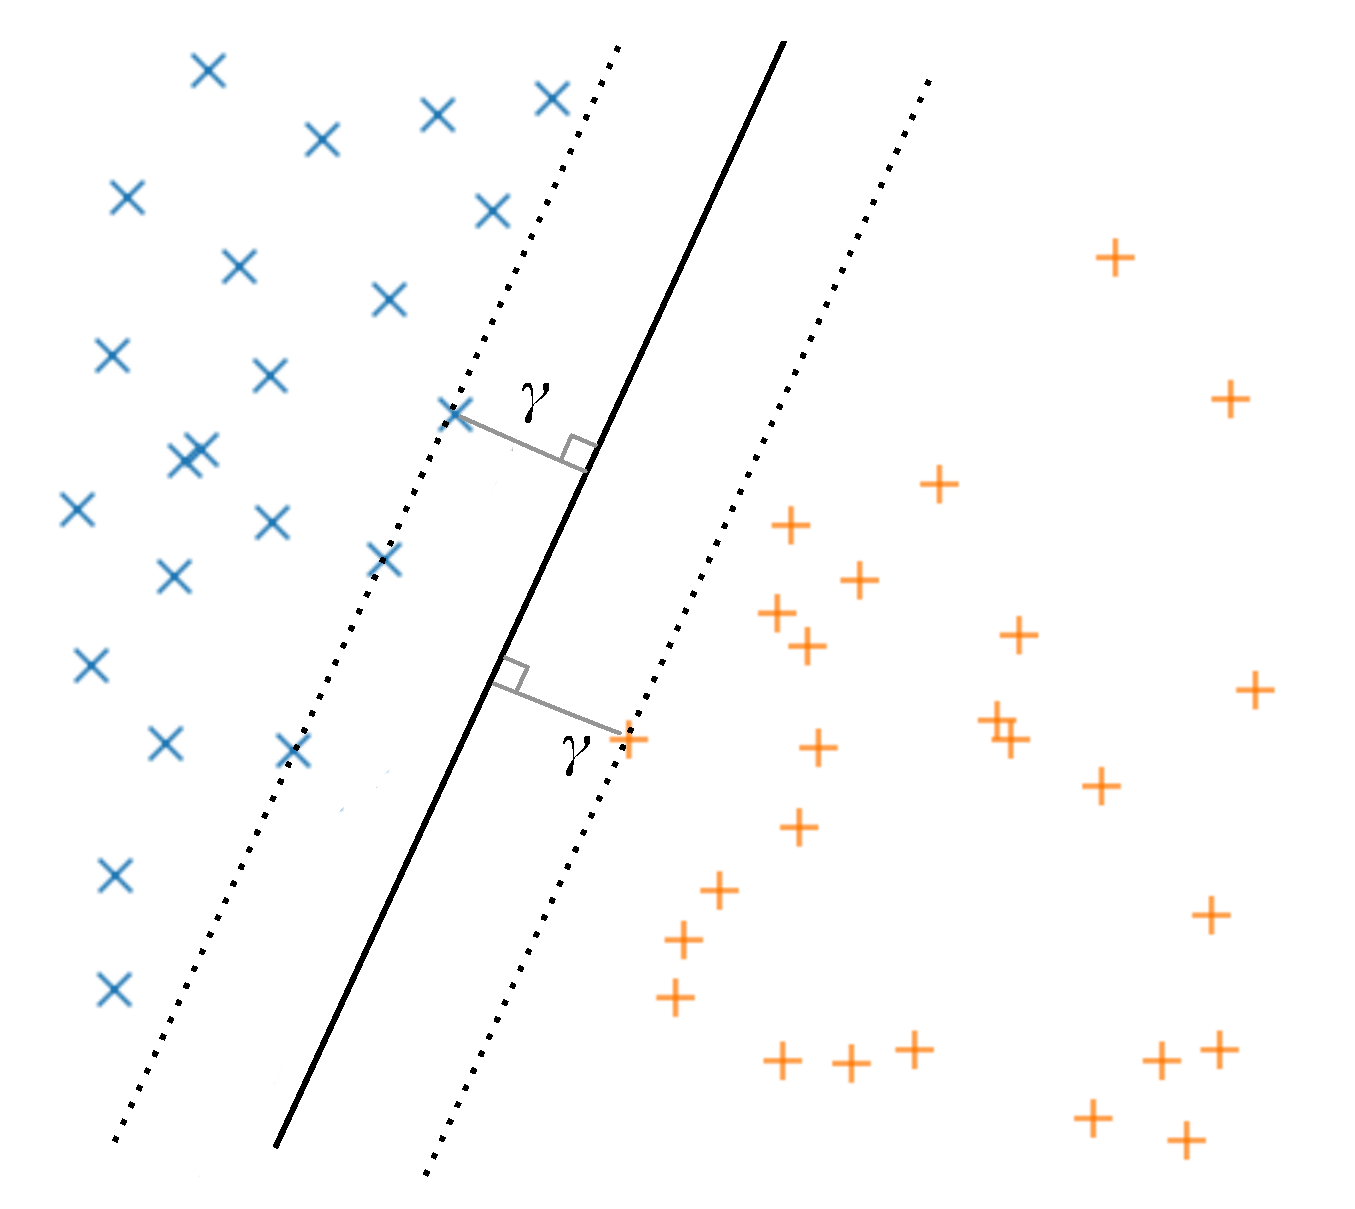
\includegraphics[width=0.43\textwidth,clip]{Images/marge6b.pdf}};
%				\node (ref) [visible on=<7>] at (0,11) {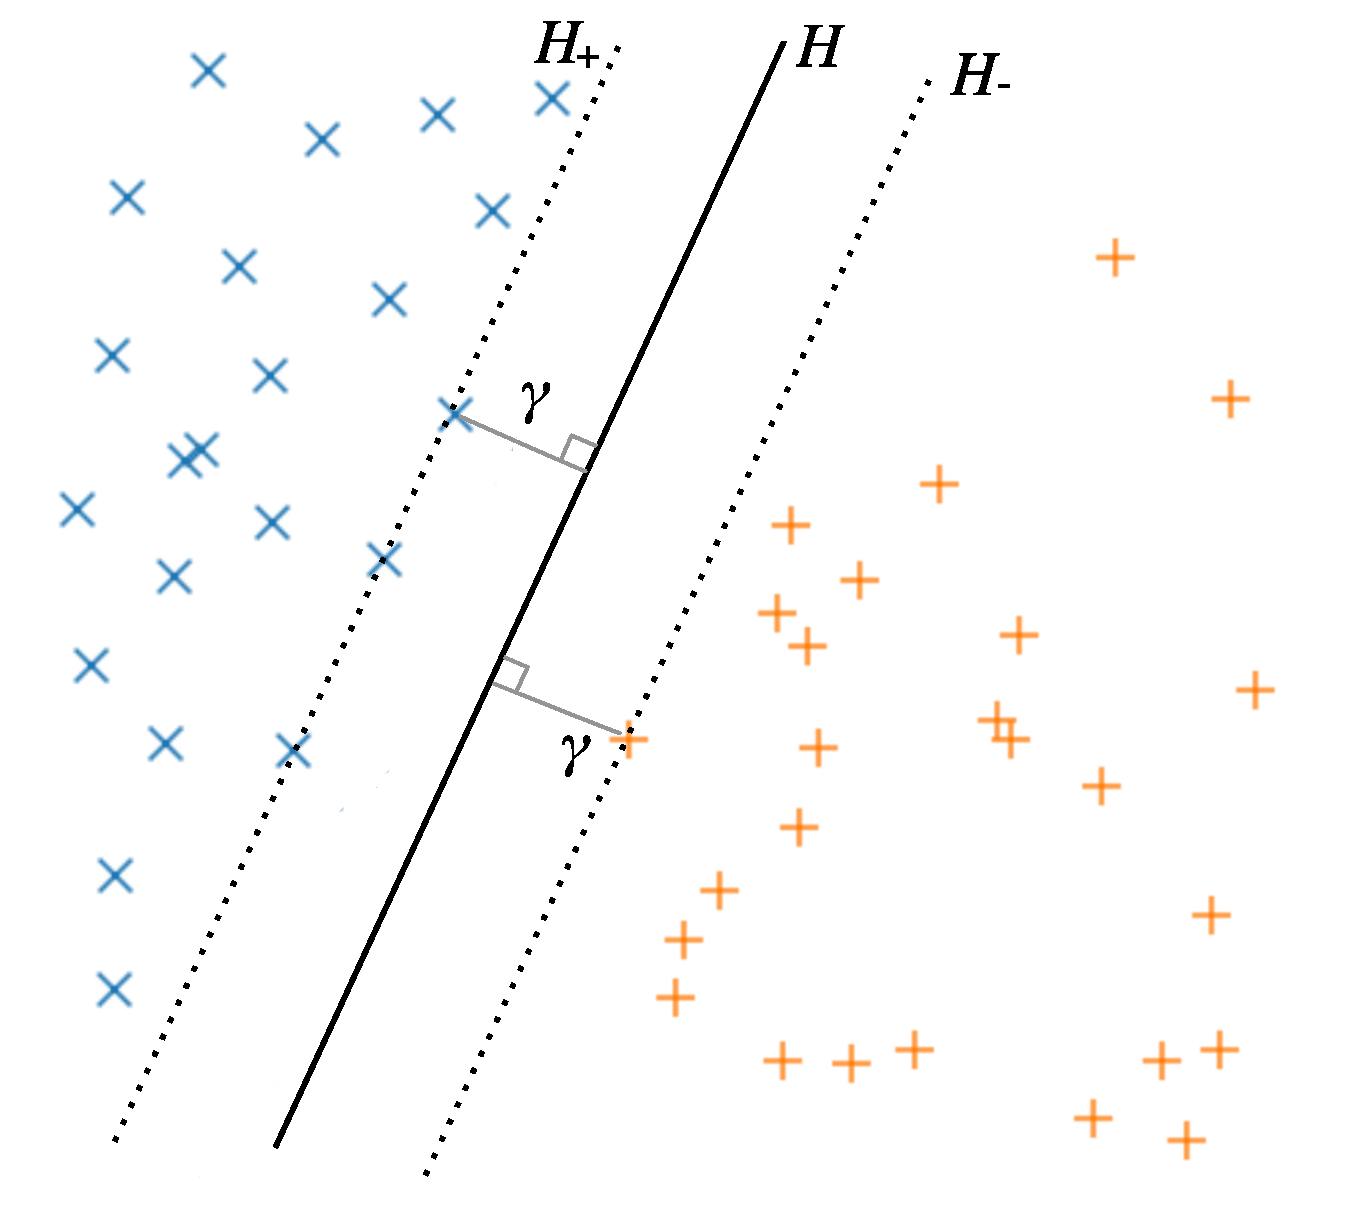
\includegraphics[width=0.43\textwidth,clip]{Images/marge7b.pdf}};
%				\node (ref) [visible on=<8>] at (0,11) {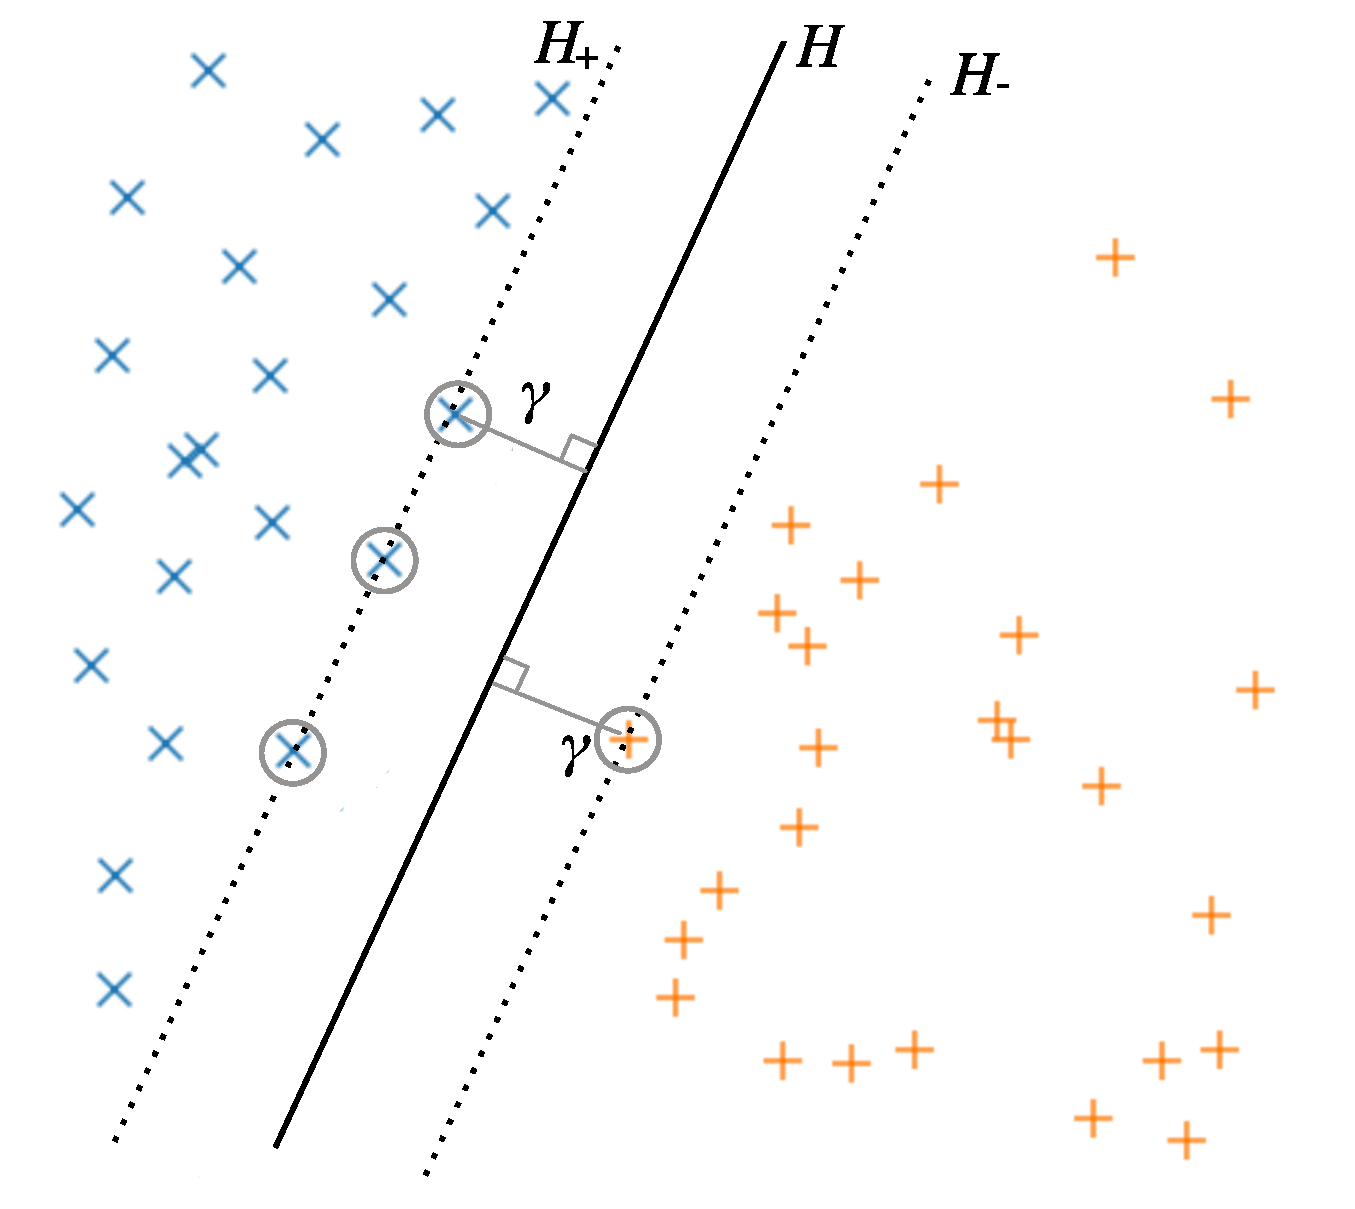
\includegraphics[width=0.43\textwidth,clip]{Images/marge8b.pdf}};
%			\end{tikzpicture}
%		\end{center}
%		
%	\end{minipt}
%	
%	%------------------------NOTE
%	\note{l'hyperplan pour lequel il y a au moins une observation négative et\une observation positive qui sont à une distance $\gamma$ de cet hyperplan}
%\end{frame}

%
%
%
%\begin{frame}{Marges et vecteurs supports}
%	\begin{minipt}[1]{0.36}	
%		\textcolor{MPTblue}{\large\textbf{Définition}}	
%		\begin{vblock}{}
%			La marge $\gamma$ d’un hyperplan séparateur est la distance de cet hyperplan à
%			l’observation du jeu d’apprentissage la plus proche.
%		\end{vblock}
%		
%		\only<1->{
%			\bftitle{Objectif} \hsp Chercher l'hyperplan séparateur qui maximise la marge $\gamma$ \uncover<1->{ \ie\\ \phantom{\bftitle{Objectif} \hsp}l'hyperplan pour lequel il y a au moins une observation négative et\\ \phantom{\bftitle{Objectif} \hsp}une observation positive qui sont à une distance $\gamma$ de cet hyperplan}
%		}
%	\end{minipt}
%	
%	\begin{minipt}[1]{0.54}	
%	\begin{center}
%	\begin{tikzpicture}
%		\node (ref) [visible on=<1>] at (0,11) {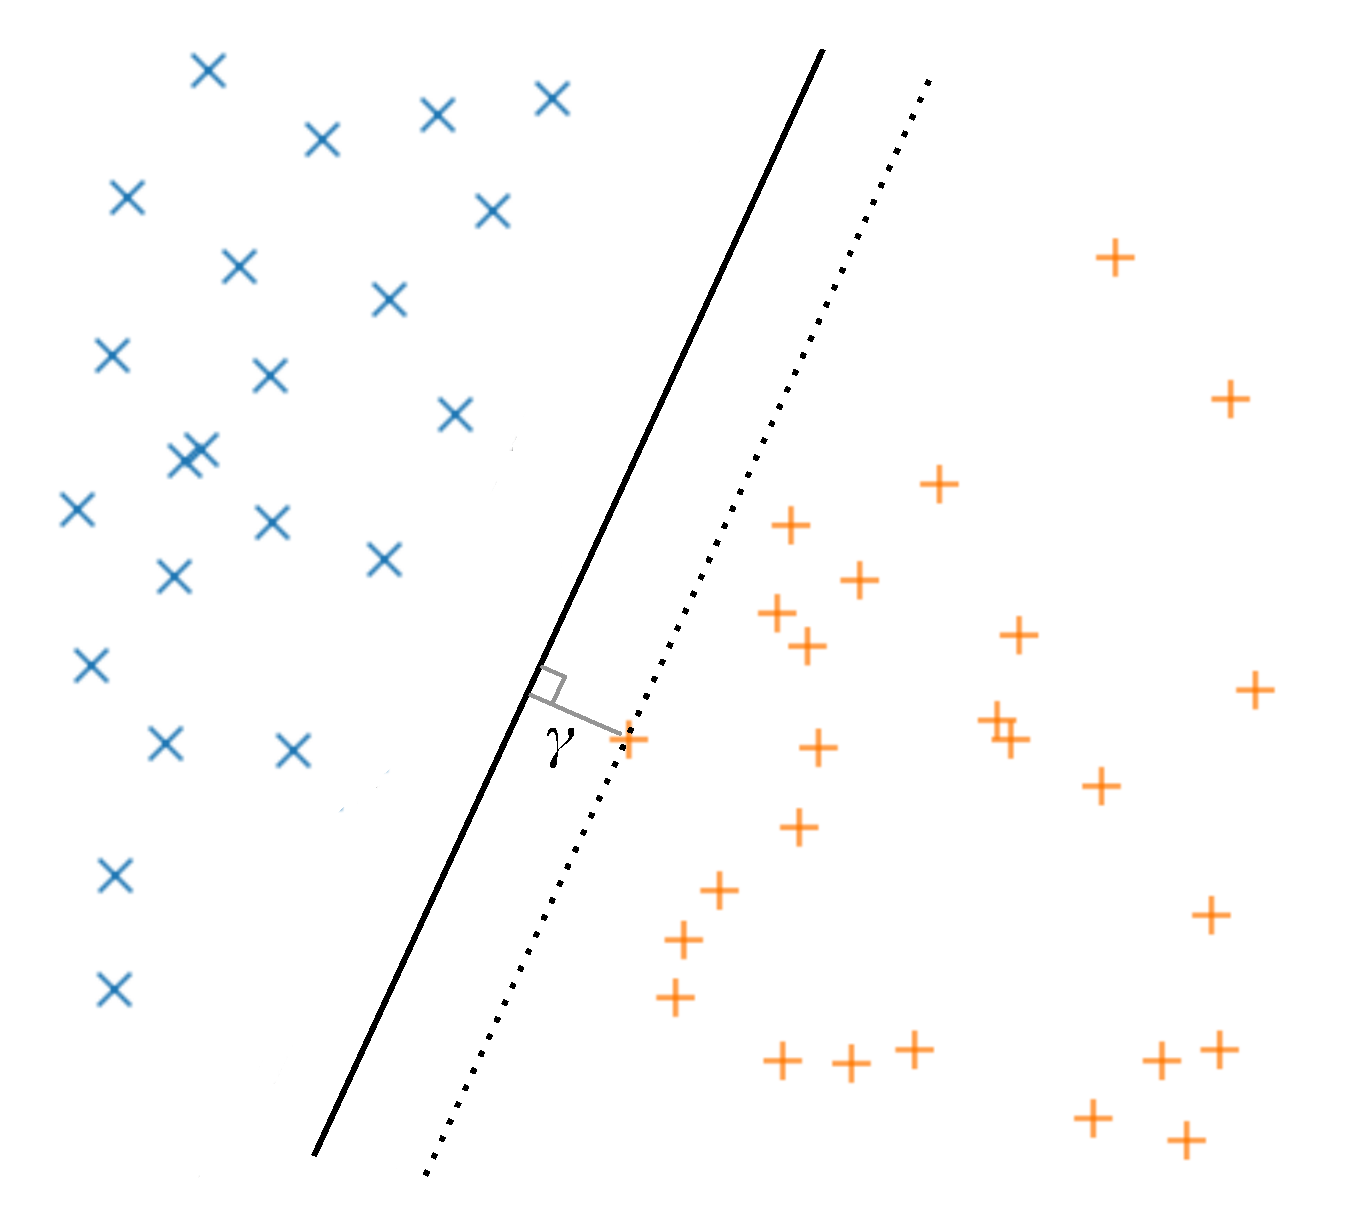
\includegraphics[width=0.43\textwidth,clip]{Images/marge1.pdf}};
%		\node (ref) [visible on=<2>] at (0,11) {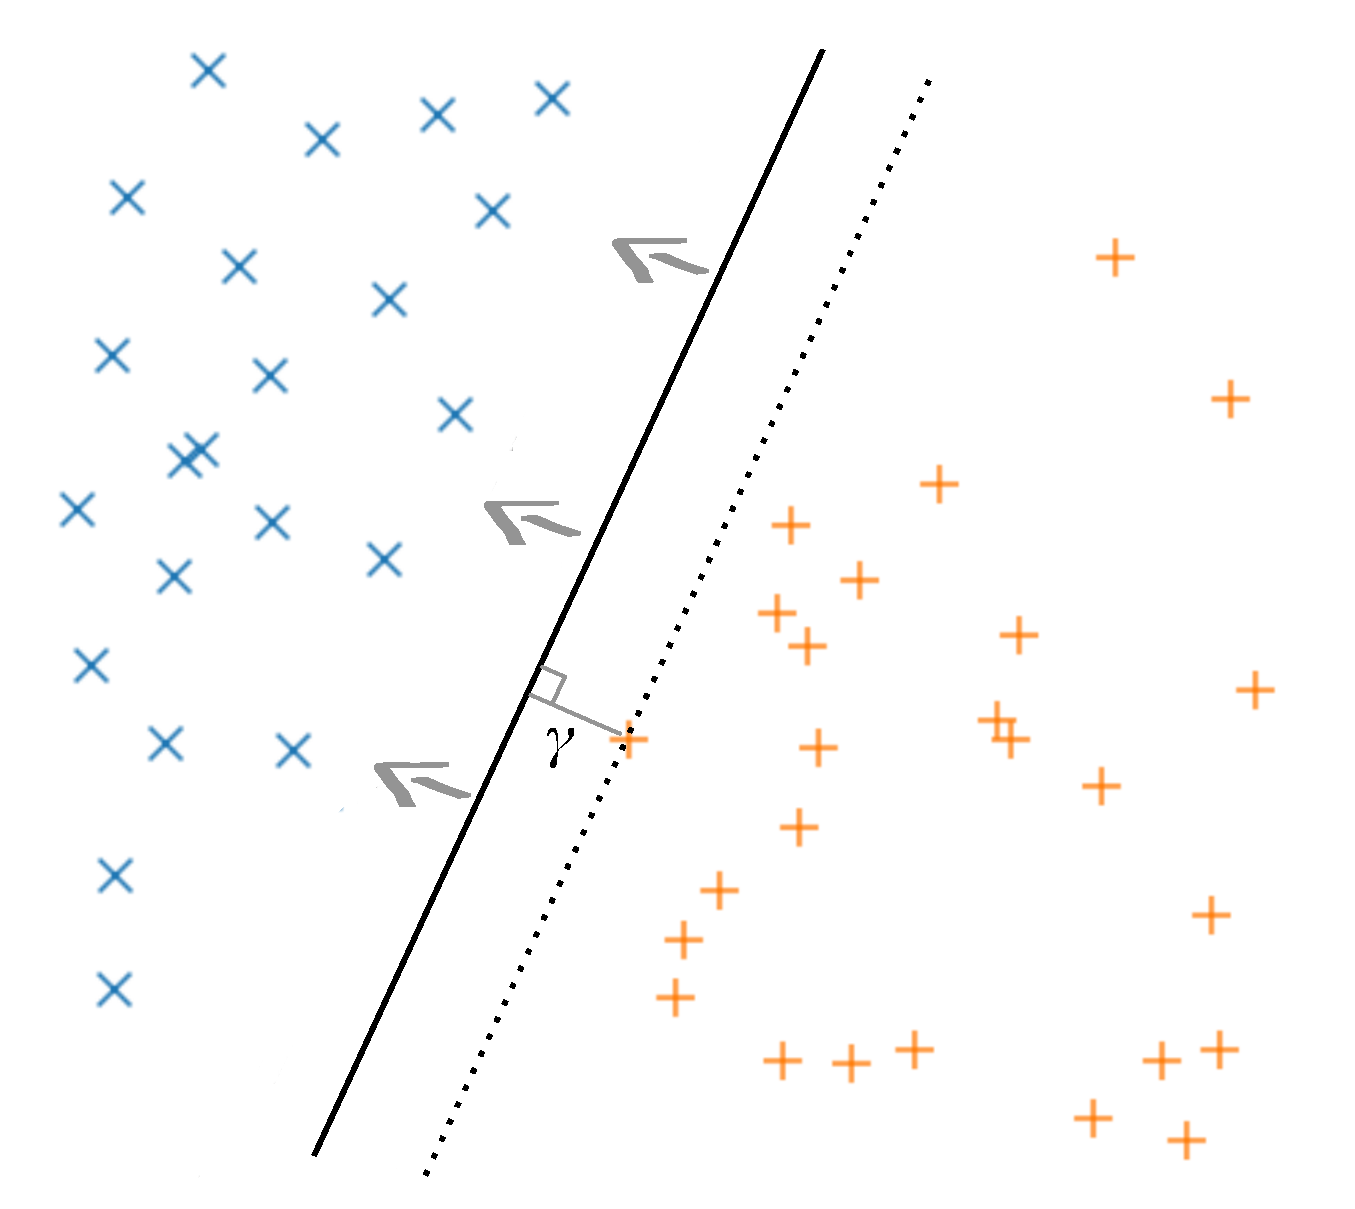
\includegraphics[width=0.43\textwidth,clip]{Images/marge2.pdf}};
%		\node (ref) [visible on=<3>] at (0,11) {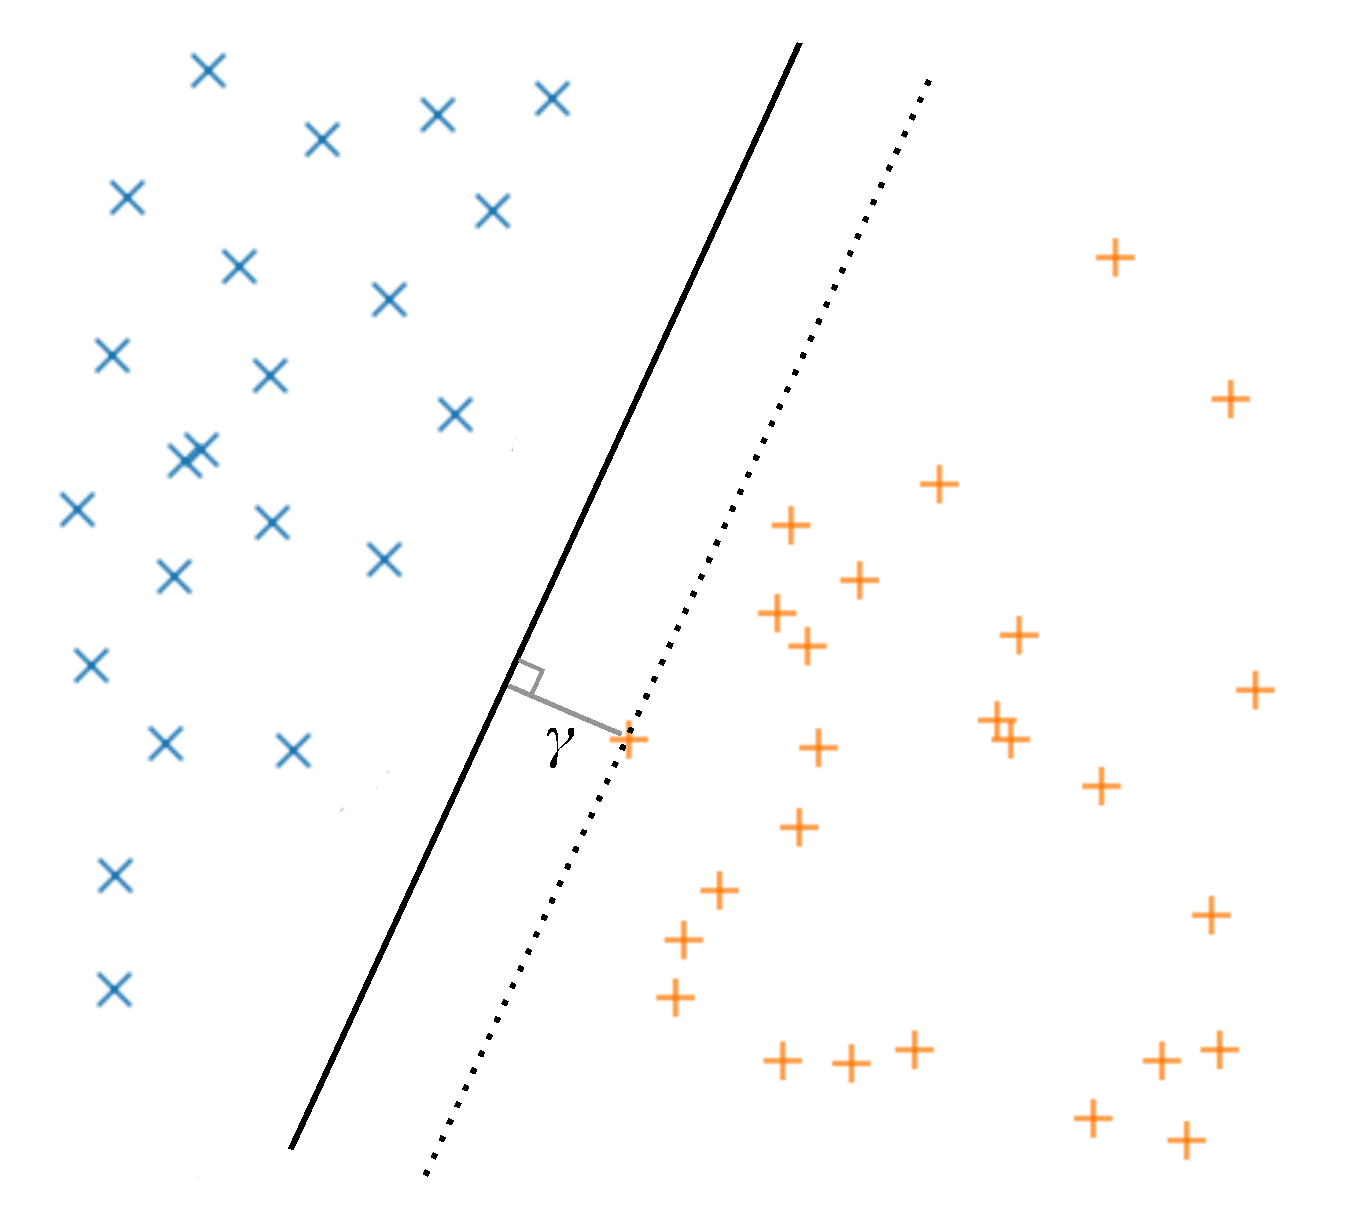
\includegraphics[width=0.43\textwidth,clip]{Images/marge3.pdf}};
%		\node (ref) [visible on=<4>] at (0,11) {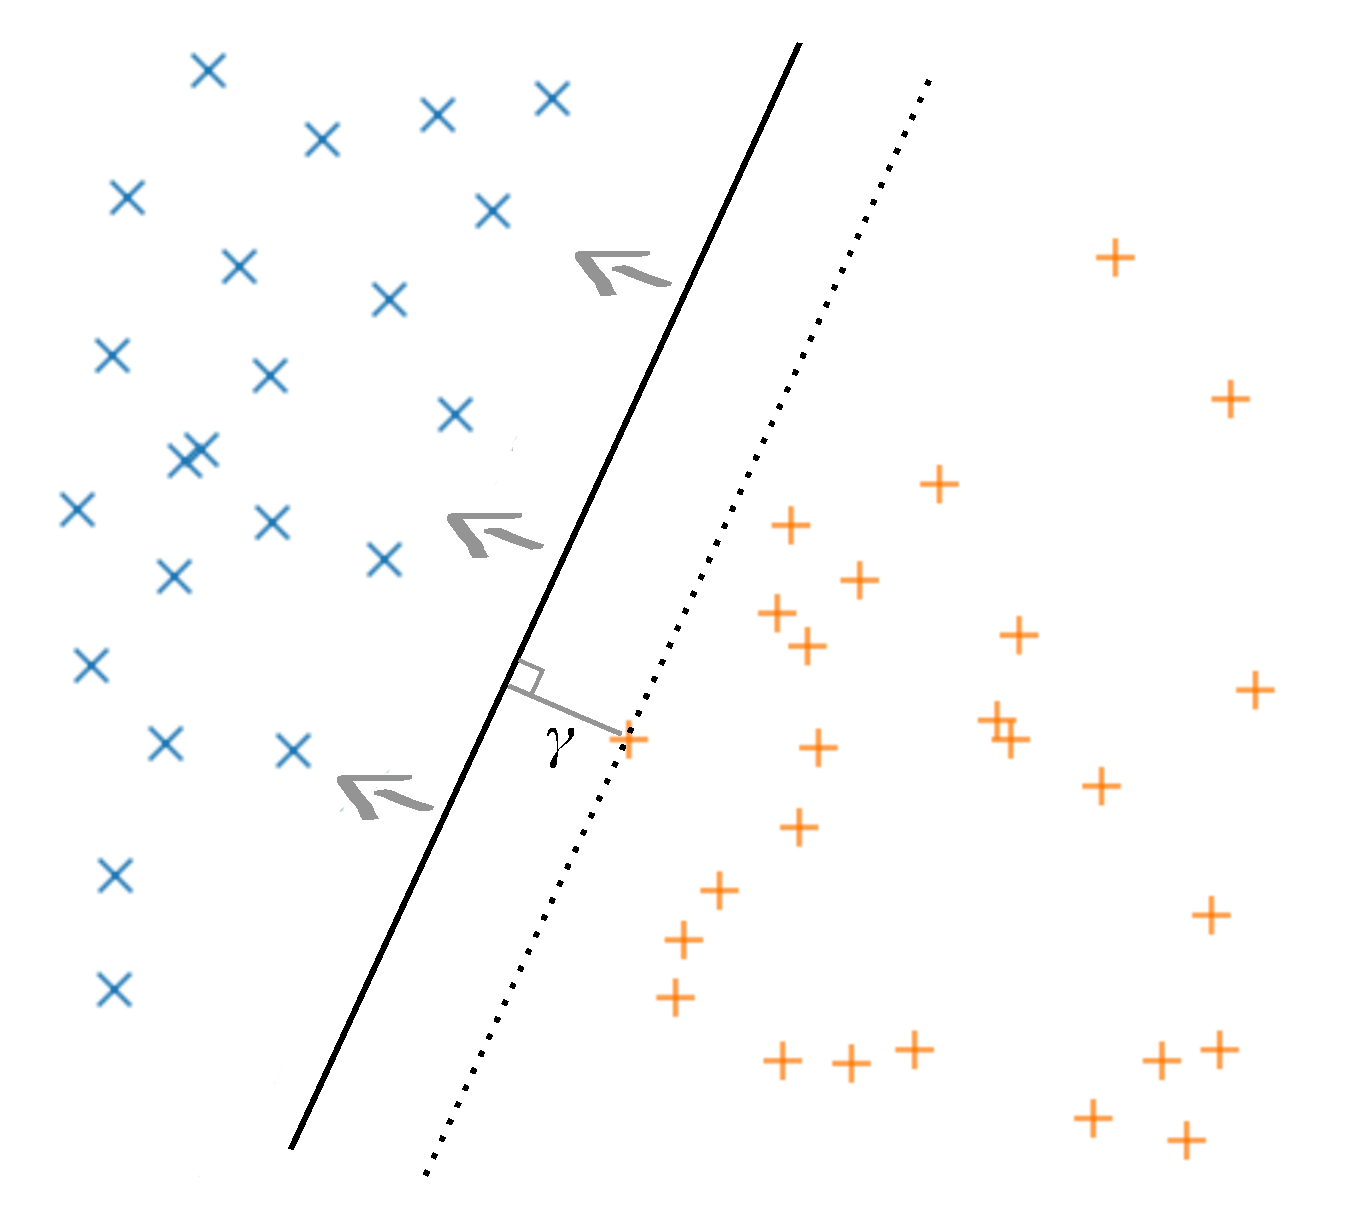
\includegraphics[width=0.43\textwidth,clip]{Images/marge4.pdf}};
%		\node (ref) [visible on=<5>] at (0,11) {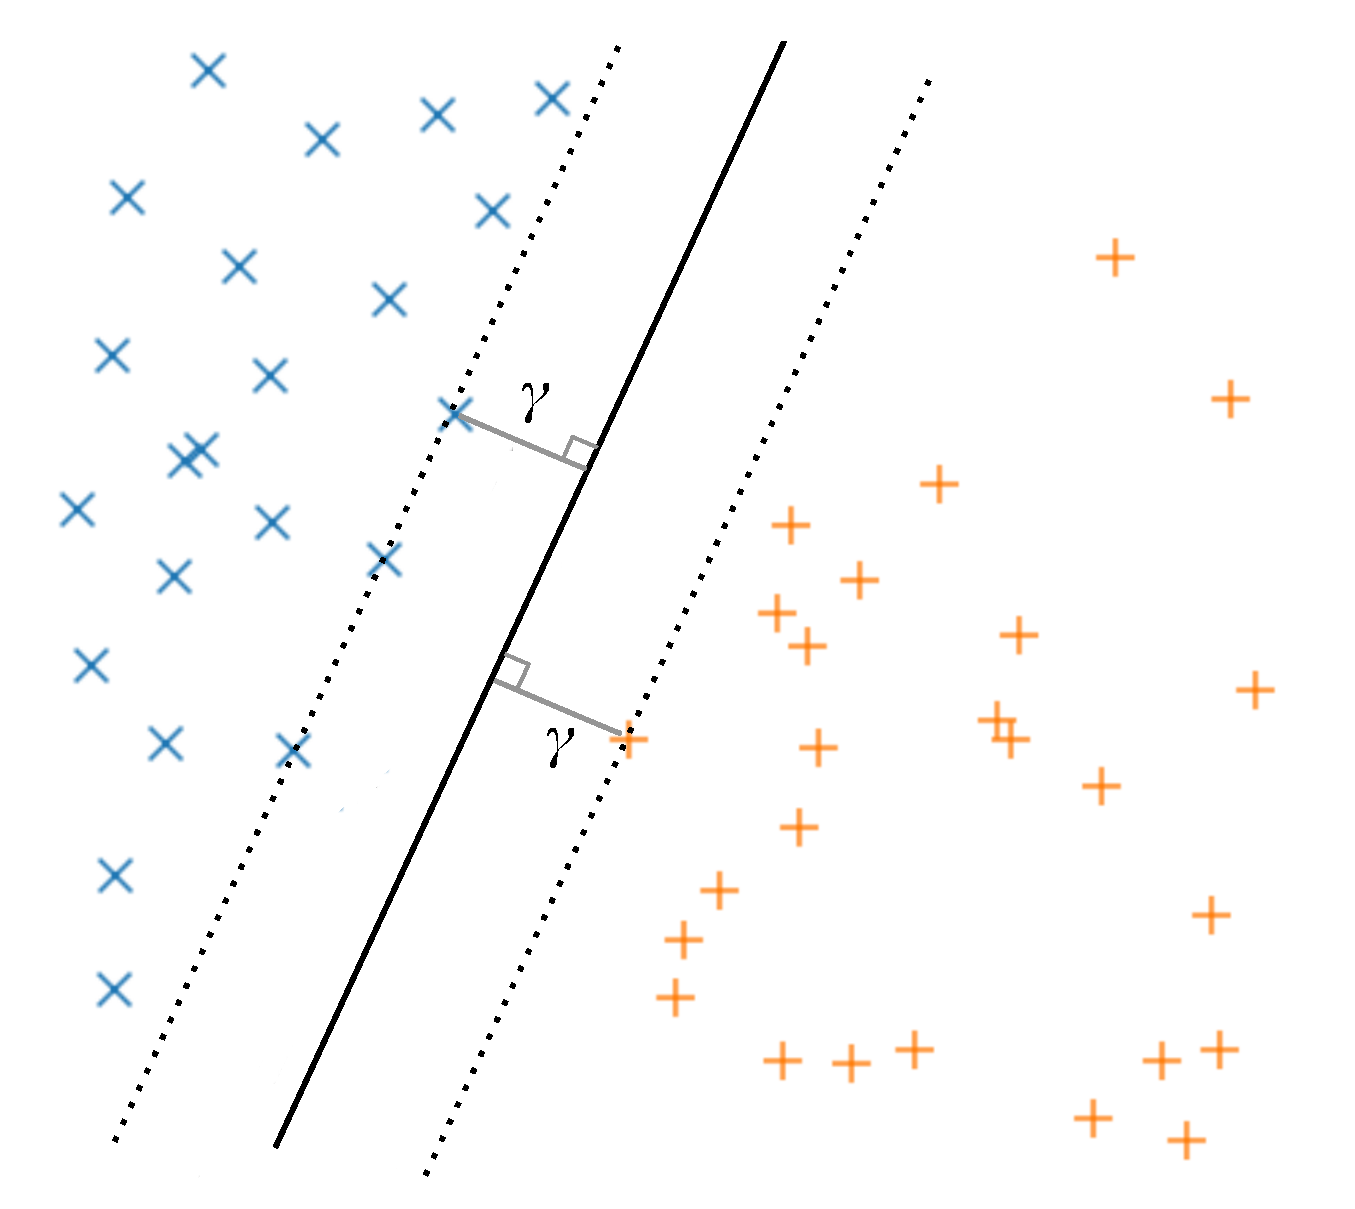
\includegraphics[width=0.43\textwidth,clip]{Images/marge5.pdf}};
%	\end{tikzpicture}
%\end{center}
%	\end{minipt}
%\end{frame}
%------------------------------------------------------------------------------------------
%------------------------------------------------------------------------------------------
\begin{frame}{Formulation mathématique}
	\vspace{-1.3em}	
Soit $(x_1,y_1),\dots,(x_n,y_n) \in \bbR^d \times \{-1,1\}$ des données %\phantom{\bftitle{Contexte} \hsp}
d'apprentissage séparables\\[1em]
	
	\bftitle{Question} \hsp Comment trouver l'hyperplan séparateur H qui maximise la marge ?\\[0.8em]
	%\\\phantom{\bftitle{Question} \hsp }On a besoin de reformuler mathématiquement le problème\\[1em]
	
	\bftitle{Rappel} \hsp Tout hyperplan $H \subset \bbR^d$ est donné par $H = \left\{x \in \bbR^d, \langle w,x\rangle + b = 0\right\}$\\
	\phantom{\bftitle{Rappel} \hsp}avec $(w,b) \in \bbR^d \times \bbR$\\[1em]
	
	\begin{minipc}[0.06]{0.15}
	%\begin{center}
	\raisebox{1.5mm}{\bclampe \xspace} 
\end{minipc}
\begin{minipc}[0.93]{0.15}
	On va reformuler le problème mathématiquement : trouver un hyperplan  séparateur $H$ qui maximise la marge revient à trouver les paramètres $w$ et $b$ adéquates, \ie qui respectent certaines conditions.
\end{minipc}	

\vspace*{1em}

		\textcolor{MPTred}{\large\textbf{Proposition}} \hfill  $\color{MPTgrey}\|\cdot\|$ \textcolor{MPTgrey}{: dist. euclidienne}\\
\vspace*{-0.2em}	
\begin{valblock}{}
Soit un hyperplan $H \subset \bbR^d$ d'équation $\langle w,x\rangle + b = 0$ avec $(w,b) \in \bbR^d \times \bbR$. La distance entre un point $x \in \bbR^d$ et $H$, \ie la distance entre $x$ et son projeté orthogonal sur $H$ est donnée par 
\vspace{-0.5em}	
$$ d(x,H) = \dfrac{\vert \langle w,x \rangle +b \vert}{\| w\|} $$
\vspace{-1.3em}	
\end{valblock}
%\textcolor{MPTgrey}{Éléments de preuve : voir \href{https://www.alloschool.com/assets/documents/course-227/sous-espaces-affines-cours.pdf}{ce cours}, page 293 }

	
\end{frame}
%------------------------------------------------------------------------------------------
%------------------------------------------------------------------------------------------


%------------------------------------------------------------------------------------------
%------------------------------------------------------------------------------------------
\begin{frame}{}
\textbf{Preuve} \clrcite{(n'est pas à savoir)}\\[2em]

Soit $x\in \bbR^d$ et $p$ son projeté orthogonal sur l'hyperplan $H$ d'équation $\langle w,x\rangle + b = 0$\\[1em]  

Puisque $\overrightarrow{xp} $ et $ \overrightarrow{w}$ sont colinéaires, alors 

$$ \overrightarrow{xp} = k\cdot \overrightarrow{w}, $$ 
avec $k =- \dfrac{\langle w,x\rangle +b}{\| w\|^2}$ \clrcite{(voir partie sur la régression logistique)} \\[1em]

Ainsi, $\|\overrightarrow{xp}\| = k \|\overrightarrow{w}\| = \dfrac{\vert \langle w,x \rangle +b \vert}{\| w\|}$\\[10em]
	
\end{frame}
%------------------------------------------------------------------------------------------
%------------------------------------------------------------------------------------------



%\begin{frame}{Formulation}
%	\bftitle{Contexte} \hsp Soit $(x_1,y_1),\dots,(x_n,y_n) \in \bbR^d \times \{-1,1\}$ un jeu de données\\ \phantom{\bftitle{Contexte} \hsp}d'apprentissage séparable et $H$ l'hyperplan séparateur qui\\ \phantom{\bftitle{Contexte} \hsp} maximise la marge  \\[1em]
%
%\textbf{\textcolor{MPTblue}{Classifieur SVM à marge rigide} }\hsp  $f(x) = \text{sign} \left[\langle \widehat{w},x\rangle+ \widehat{b} \right]$\\
%\phantom{\textbf{\textcolor{MPTblue}{Classifieur SVM à marge rigide} }\hsp} \uncover<2->{avec $\langle \widehat{w},x\rangle+ \widehat{b}=0$, $\forall x \in H$}\\[1em]
%%	\textbf{\textcolor{MPTblue}{Classifieur SVM à marge rigide} }:\\
%%\phantom{a} \hfill	$f(x) = \text{sign} \left[\langle \widehat{w},x\rangle+ \widehat{b} \right]$ \hsp  avec $\langle \widehat{w},x\rangle+ \widehat{b}=0$ pour tout $x \in H$ \hfill \phantom{a}\\[1em]
%
%\uncover<3>{	
%	\bftitle{Question} \hsp Comment trouver $(\widehat{w},\widehat{b})$ ? On a besoin de reformuler\\\phantom{\bftitle{Question} \hsp }mathématiquement le problème\\[1em]
%}
%
%\end{frame}
%------------------------------------------------------------------------------------------
%------------------------------------------------------------------------------------------
%\begin{frame}{Formulation mathématique}
%	
%\textcolor{MPTred}{\large\textbf{Proposition}}\hfill \textcolor{MPTgrey}{SVM à marge rigide}\\
%\vspace*{-0.2em}	
%\begin{valblock}{}
%	Soit $(\widehat{w}, \widehat{b}) \in \bbR^d \times \bbR$ des paramètres qui vérifient
%	\begin{equation}\label{eq:optim1}
%		 (\widehat{w}, \widehat{b}) = \underset{\substack{(w,b) \in \bbR^d\times\bbR \\ \|w\|_2=1}}{\text{{arg}}\,\max}\,\,\min\limits_{i \in \llbracket1,n\rrbracket} \, \, yi\left(\langle w,xi \rangle +b\right)
%	  \end{equation}
%Alors $H =\big\{x \in \bbR^d, \langle \widehat{w},x\rangle + \widehat{b} = 0\big\}$ est un hyperplan séparateur qui maximise la marge
%\end{valblock}
%
%	\begin{minipc}[0.06]{0.15}
%	\warning
%\end{minipc}
%\begin{minipc}[0.93]{0.15}
%	La contrainte $\|w\|_2=1$ est non convexe. Il est donc plus difficile de résoudre numériquement le programme d'optimisation ci-dessous
%\end{minipc}
%
%	\begin{minipc}[0.06]{0.15}
%	%\begin{center}
%	\raisebox{1.5mm}{\bclampe \xspace} 
%\end{minipc}
%\begin{minipc}[0.93]{0.15}
%	On va essayer de reformuler ce problème d'optimisation pour avoir une expression plus facile à résoudre
%\end{minipc}
%
%\end{frame}
%------------------------------------------------------------------------------------------
%------------------------------------------------------------------------------------------
\begin{frame}{Formulation primale}
	\vspace*{-0.6em}
	\begin{minipt}[1]{0.5}
	
	\textcolor{MPTred}{\large\textbf{Proposition}}\hfill \textcolor{MPTgrey}{SVM à marge rigide}\\
	\vspace*{-1.1em}	
	\begin{valblock}{}
		Soit $(\widehat{w}, \widehat{b}) \in \bbR^d \times \bbR$ des paramètres qui vérifient
		\begin{equation}\label{eq:optim2}
			(\widehat{w}, \widehat{b}) = \underset{(w,b) \in \bbR^d\times\bbR }{\text{{arg}}\,\min}\,\, \dfrac{1}{2} \|w\|^2 \hsp \text{s.c.} \hsp  y_i\left(\langle w,x_i \rangle +b\right) \geq 1 \hsp  \forall i \in \{1,\dots,n\} 
		\end{equation}
		Alors $H =\big\{x \in \bbR^d, \langle \widehat{w},x\rangle + \widehat{b} = 0\big\}$ est un hyperplan séparateur qui maximise la marge. En particulier, il existe $ i,j \in \{1,\dots,n\}$ tels que $x_i \in H_+ = \big\{x \in \bbR^d, \langle \widehat{w},x\rangle + \widehat{b} = 1 \big\}$ et $x_j \in H_-= \big\{x \in \bbR^d, \langle \widehat{w},x\rangle + \widehat{b} = -1 \big\}$
	\end{valblock}
\end{minipt}



\begin{minipt}[1]{0.47}
	\only<1>{
		\vspace*{2em}
		
\begin{itemize}
	\item Le problème défini par \eqref{eq:optim2} est un \textbf{problème d'optimisation convexe} %($w\mapsto \dfrac{1}{2} \|w\|_2^2$ est convexe et les contraintes $(w,b) \mapsto 1- yi\left(\langle w,xi \rangle +b\right)$ sont des fonctions affines) 
	%s'il admet une solution
	\\[0.8em]
	\item Le problème défini par \eqref{eq:optim2}  est un \textbf{problème d'optimisation quadratique }
	%($w\mapsto \dfrac{1}{2} \|w\|_2^2$ est convexe et les contraintes $(w,b) \mapsto 1- yi\left(\langle w,xi \rangle +b\right)$ sont des fonctions affines) 
	: de nombreuses solutions ont été proposées pour résoudre ce type de problème\\[0.8em]
%	\item Tout hyperplan d'équation $\langle w,x\rangle +b = 0$ est invariant à une multiplication près des coefficients $w$ et $b$ par $k \in \bbR^*$. Les solutions données par l'équation \eqref{eq:optim2} définissent donc le même hyperplan $H$  
 
\end{itemize}
}

\only<2->{
	\vspace*{0.5em}
\bftitle{Question} \hsp Quelle étiquette attribuer à un nouveau point $x \in \bbR^d$ ?\\[0.8em]


\uncover<3>{
	\textbf{\textcolor{MPTblue}{Classifieur SVM à marge rigide} }:\\
$$\text{sign} \left[\langle \widehat{w},x\rangle+ \widehat{b} \right]$$
avec $(\widehat{w}, \widehat{b})$ la solution donnée par  l'équation \eqref{eq:optim2} 
}
}
\end{minipt}	
\end{frame}
%------------------------------------------------------------------------------------------
%------------------------------------------------------------------------------------------

\begin{frame}{Formulation duale}
		\only<1>{
			\vspace*{-1em}
	%	\begin{minipt}[1]{0.99}
	%	\vspace*{0.1em}
		\textcolor{MPTred}{\large\textbf{Proposition}}\hfill \textcolor{MPTgrey}{SVM à marge rigide}\\
	\vspace*{-0.2em}		
		\begin{valblock}{}
			Soit $\widehat{\alpha} = (\widehat{\alpha}_1, \dots,\widehat{\alpha}_n) \in \bbR^n$ qui vérifie
			\begin{equation}
				\begin{array}{lll}
				\widehat{\alpha}& =& \displaystyle \underset{\alpha=(\alpha_1,\dots,\alpha_n) \in \bbR^n}{\text{{arg}}\,\max}\,\, \sum_{i=1}^n \alpha_i  - \dfrac{1}{2} \sum_{i=1}^n \sum_{i=\ell}^n \alpha_i\alpha_\ell \ y_i y_\ell \  \langle x_i,x_\ell\rangle\\				
				&& \text{s.c.} \sum_{i=1}^n \alpha_i y_i = 0 \text{ et } \alpha_i \geq 0 \hsp \forall i \in \{1,\dots,n\}  
				\end{array}
			\label{eq:optim3}
			\end{equation}
		
	Alors le couple $(\widehat{w}, \widehat{b})$ défini par
		$$ \widehat{w}= \sum_{i=1}^n  \widehat{\alpha}_i y_i x_i \hsp \hsp \text{et} \hsp \hsp \widehat{b}= 1-\min\limits_{\substack{i \in \{1,\dots, n \} \\ y_i = 1}} \langle\widehat{w},x_i \rangle $$
		est identique à la solution donnée par l'équation \eqref{eq:optim2}
		\end{valblock}
	\textcolor{MPTgrey} {Preuve : section 10.1.3 d'\textit{\href{http://cazencott.info/dotclear/public/lectures/IntroML_Azencott.pdf}{Introduction au Machine Learning}} de Chloé-Agathe Azencott} \\[1em]
	
			\textbf{\textcolor{MPTblue}{Classifieur SVM à marge rigide}} \hsp  $ 
	 \text{sign} \left[ \sum_{i =1}^n \hat{\alpha}_i y_i \langle x_i,x\rangle  + \widehat{b} \right]$
	
%	\end{minipt}
}
\only<2>{
		\vspace*{-0.5em}
%	\begin{itemize}
		 Le problème défini par \eqref{eq:optim3} est un \textbf{problème d'optimisation convexe et quadratique}. Il est appelé \textit{problème d'optimisation dual} et est obtenu à partir du \textit{problème d'optimisation primal} défini par \eqref{eq:optim2} de la manière suivante : \\[1em] 
%\end{itemize}

 Le problème primal $(P)$ induit par \eqref{eq:optim2} peut se réécrire à l'aide de son Lagrangien $\L$ : 
 $$(P) :  \hsp   \underset{(w,b) \in \bbR^d\times\bbR }{\min}\hsp \underset{\substack{\alpha=(\alpha_1,\dots,\alpha_n) \in \bbR^n\\
		\alpha_1 \geq 0, \dots, \alpha_n \geq 0 }}{\max}\,\, \L\left(w,b, \alpha\right) $$
	\vspace*{-1em}
	
où $\L(w,\alpha) = \dfrac{1}{2} \|w\|^2  + \sum_{i=1}^n \alpha_i \big(1-y_i\langle w,x_i\rangle\big)$\\[1.5em]

En inversant le $\min$ et le $\max$ dans $(P)$ on obtient le problème dual $(Q)$ suivant :
$$ (Q) :  \hsp   \underset{\substack{\alpha=(\alpha_1,\dots,\alpha_n) \in \bbR^n\\
		\alpha_1 \geq 0, \dots, \alpha_n \geq 0 }}{\max} \hsp  \underset{(w,b) \in \bbR^d\times\bbR }{\min}\, \,  \L\left(w,b, \alpha\right) $$
		\vspace*{-1em}
		
De manière générale, n'importe quelles solutions ${p^*}$ de $(P)$ et ${q^*}$ de $(Q)$ vérifient toujours $q^* \leq p^*$ (dualité faible) mais puisque $(P)$ est un problème d'optimisation convexe avec des contraintes affines alors on a $p^*=q^*$ (condition de Slater), \ie, le saut de dualité $p^*-q^*$ est nulle
}

\only<3->{
	\vspace*{-0.5em}
	%		\vspace*{-1.5em}
	%		\begin{equation}\label{eq:optim3}
		%		\begin{array}{lll}
			%			\widehat{\alpha}& =& \underset{\alpha=(\alpha_1,\dots,\alpha_n) \in \bbR^n}{\text{{arg}}\,\max}\,\, \sum_{i=1}^n \alpha_i  - \dfrac{1}{2} \sum_{i=1}^n \sum_{i=1}^\ell \alpha_i\alpha_\ell \ y_i y_\ell \  \langle x_i,x_\ell\rangle\\				
			%			&& \text{s.c.} \sum_{i=1}^n \alpha_i y_i \text{ et } \alpha_i \geq 0 \hsp \forall i \in \{1,\dots,n\}  
			%		\end{array}
		%	\end{equation}	
	%	$$ \widehat{w}= \sum_{i=1}^n \alpha_i y_i x_i \hsp \hsp \text{et} \hsp \hsp \widehat{b}= 1-\min\limits_{\substack{i \in \{1,\dots n \} \\ y_i = 1}} \langle\widehat{w},x_i \rangle $$	
	\begin{itemize}
		\item \textbf{Interprétation géométrique} : les solutions $	\widehat{\alpha}$ et $(\widehat{w},\widehat{b})$ vérifient les \textit{conditions d'optimalité de Karush-Kuhn-Tucker} dont la \textit{condition d'écart complémentaire} qui stipule que, pour tout $i \in \llbracket1,n\rrbracket$, $\widehat{\alpha}_i \left[y_i\left(\langle\widehat{w}, x_i\rangle + \widehat{b}\right) - 1\right] = 0$. Il y a alors deux possibilités, \textcolor{MPTgrey}{lesquelles} ?\\[0.5em]
		
		\uncover<4>{			
			\begin{itemize}
				\item[\ex] \hsp Si $x_i$ est \textit{à l'extérieur} des hyperplans $H_+$ et $H_{-}$, \ie $y_i\left(\langle\widehat{w}, x_i\rangle + \widehat{b}\right) > 1$\\ \hsp alors $\widehat{\alpha}_i=0$\\[0.5em]
				
				\item[\ex] \hsp Si $\widehat{\alpha}_i>0$ alors $y_i\left(\langle\widehat{w}, x_i\rangle + \widehat{b}\right)=1$, \ie $x_i \in H_+$ ou $x_i \in H_-$ ;\\ \hsp $x_i$ est donc un vecteur de support\\[1em]
	\end{itemize}

La formulation duale permet d'identifier des vecteurs de support (pas forcément tous). Ce sont seulement ces vecteurs de support qui sont utilisés pour construire le classifieur à marge rigide\\[1em]
}
		\item \textbf{Complexité algorithmique} : la formulation primale est un problème d’optimisation en $d + 1$ dimensions tandis que la
		formulation duale est un problème en $n$ dimensions. Avec peu de données et beaucoup de variables explicatives, on préférera la formulation duale ; dans le cas inverse, on préférera résoudre le problème primal.\\[0.5em]
		%		\item \textbf{\textcolor{MPTblue}{Classifieur SVM à marge rigide}}: \hsp  $f(x) = 
		%	\displaystyle \text{sign} \left[ \sum_{i =1}^n \alpha_i y_i \langle x_i,x\rangle  + \widehat{b} \right]$
	\end{itemize}
}

	\note{Si bien sûr on a au moins une observation de chaque classe mais sinon pas de problème donc pas dur à supposer}
\end{frame}
%------------------------------------------------------------------------------------------
%------------------------------------------------------------------------------------------

\section{Le cas linéairement non séparable :\\[0.5em] SVM à marge souple}

%------------------------------------------------------------------------------------------
%------------------------------------------------------------------------------------------
\begin{frame}{Données non séparables linéairement}

	\begin{center}
		
		\begin{tikzpicture}
			\node (ref1) [right=of ref,visible on=<1>] {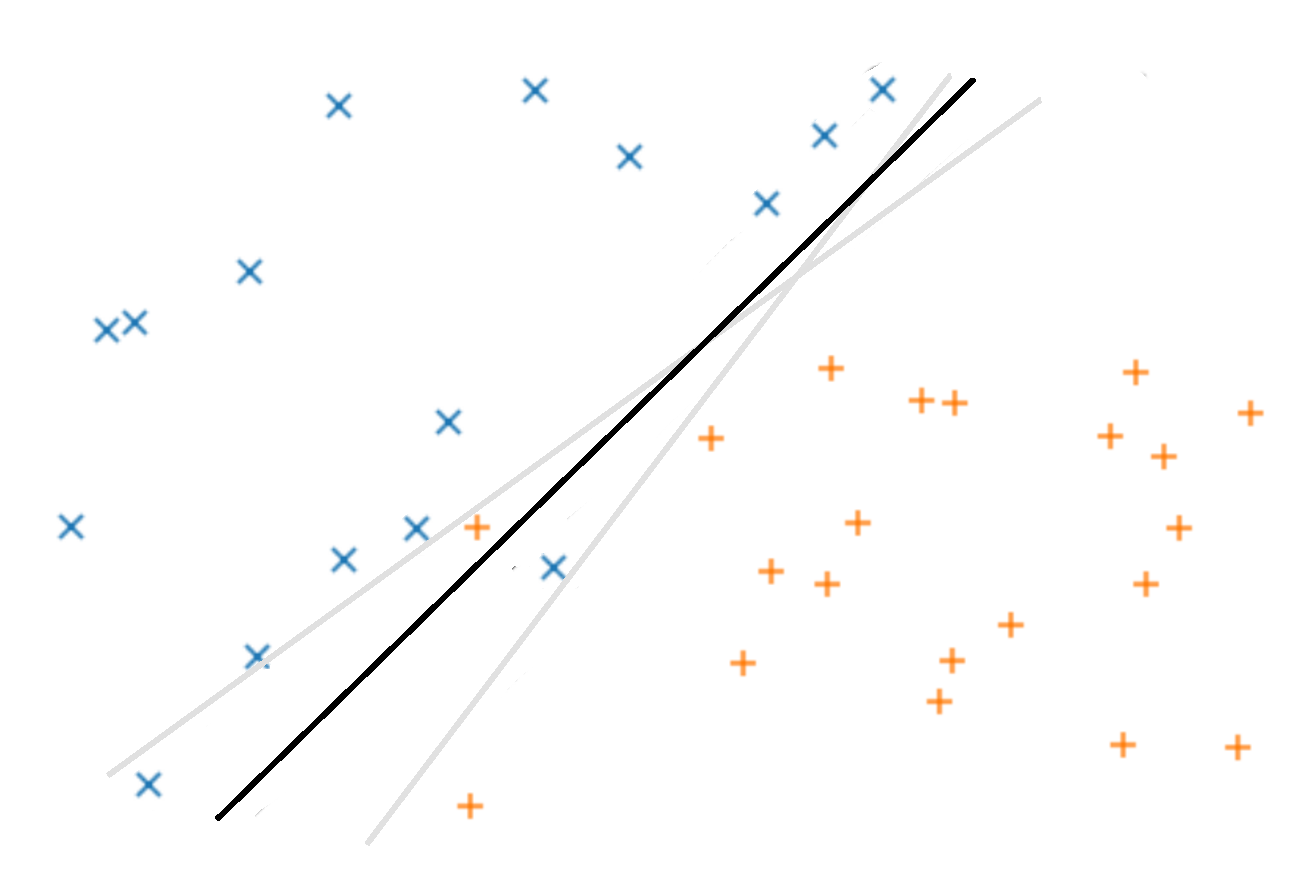
\includegraphics[width=0.55\textwidth,clip]{nonseparable3b.pdf}};
			\node (ref1) [right=of ref,visible on=<2>] {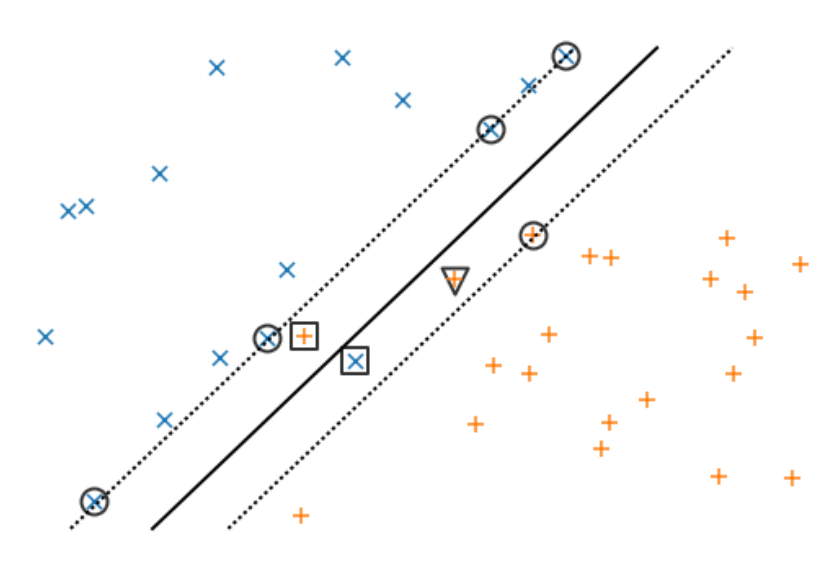
\includegraphics[width=0.55\textwidth,clip]{nonseparable1.png}};
			%\node (wiki1)[]at([xshift = 30]wiki.east) {Non séparable linéairement};
			%\node (wiki)[]  at([yshift = 27.5]ref1.north) {Non séparables linéairement};
			
		\end{tikzpicture}
		
		%\vspace*{1.5em}
		\footnotesize{\textcolor{MPTgrey}{Tirée de l'ouvrage \textit{\href{http://cazencott.info/dotclear/public/lectures/IntroML_Azencott.pdf}{Introduction au Machine Learning}} de Chloé-Agathe Azencott} }\\[1em]		
	\end{center}
	\begin{minipc}[0.06]{0.11}
	\warning
\end{minipc}
\begin{minipc}[0.93]{0.11}
	Données non séparables linéairement, mais seulement à quelques observations près (bruit ?)
\end{minipc}
\uncover<2>{
\begin{minipc}[0.06]{0.15}
	%\begin{center}
	\raisebox{1.5mm}{\bclampe \xspace} 
\end{minipc}
\begin{minipc}[0.93]{0.15}
		On va quand même séparer linéairement les données en maximisant la marge mais en autorisant maintenant quelques erreurs de classification
\end{minipc}
}
%-------NOTE
\note{si données non séparables, alors problèmes maximisation précédents n'a pas de solutions}
\end{frame}
%------------------------------------------------------------------------------------------
%------------------------------------------------------------------------------------------
\begin{frame}{Variable d'ajustement $ \color{MPTblue} \mathbf{\xi_i}$}
	\vspace*{-0.5em}
	\textbf{Contrainte de séparabilité pour les SVM à marge rigide} de l'équation \eqref{eq:optim2}, \ie tous les points du jeu d'entraînement sont bien classés : 
	\begin{equation}\label{eq:contrainte1} \forall i \in \{1,\dots, n\}\hsp \hsp y_i\left(\langle w,x_i\rangle +b \right) \geq 1
		\end{equation}
	
	\vspace*{-0.9em}	
	\textbf{Contrainte de séparabilité relachée pour SVM à marge souple}, \ie un point du jeu d'entraînement peut maintenant être dans la zone d'indécision :
	$$ \forall i \in \{1,\dots, n\}\hsp \hsp y_i\left(\langle w,x_i\rangle +b \right) \geq 1 - \xi_i$$
	où $\xi_i  \geq 0 $, appelée \textit{variable d'ajustement} (\textit{slack variable} en anglais), mesure à quel point la contrainte \eqref{eq:contrainte1} a été enfreinte, \ie à quel point $(x_i,y_i)$ échoue à être bien séparé. \textcolor{MPTgrey}{Trois cas, lequels ?} \\[0.5em]
	
	\uncover<2>{
	\begin{minipc}[0.23]{0.1}
	\ex \hsp $\xi_i= 0$
	\end{minipc}
	\begin{minipc}[0.73]{0.1}
		$y_i\left(\langle w,x_i\rangle +b \right) \geq 1$, \ie $(x_i,y_i)$ est bien classé et est en dehors de la zone d'indécision
	\end{minipc}

	\begin{minipc}[0.23]{0.1}
	\ex \hsp $0 < \xi_i\leq 1$
\end{minipc}
\begin{minipc}[0.73]{0.1}
	$0\leq y_i\left(\langle w,x_i\rangle +b \right) < 1$, \ie $(x_i,y_i)$ est bien classé mais est dans la zone d'indécision
\end{minipc}

	\begin{minipc}[0.23]{0.1}
	\ex \hsp  $\xi_i >1 $
\end{minipc}
\begin{minipc}[0.73]{0.1}
$y_i\left(\langle w,x_i\rangle +b \right) < 0$, \ie $(x_i,y_i)$ est mal classé (et peut être dans la zone d'indécision ou non)
\end{minipc}
}
\note{faire un dessin au tableau}
\end{frame}
%------------------------------------------------------------------------------------------
%------------------------------------------------------------------------------------------
\begin{frame}
	\vspace*{-1em}
	\begin{center}
		\begin{tikzpicture}
		\node (ref1) [right=of ref,visible on=<1>] {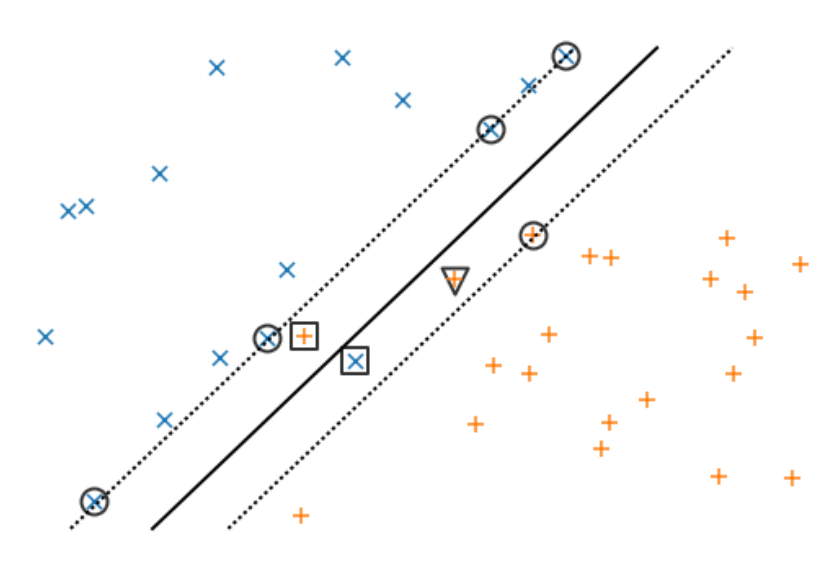
\includegraphics[width=0.55\textwidth,clip]{nonseparable1.png}};
		%\node (wiki1)[]at([xshift = 30]wiki.east) {Non séparable linéairement};
		%\node (wiki)[]  at([yshift = 27.5]ref1.north) {Non séparables linéairement};
		
	\end{tikzpicture}
	
	%\vspace*{1.5em}
%	\footnotesize{\textcolor{MPTgrey}{Tirée de l'ouvrage \textit{\href{http://cazencott.info/dotclear/public/lectures/IntroML_Azencott.pdf}{Introduction au Machine Learning}} de Chloé-Agathe Azencott} }\\[2em]	
	\end{center}
\vspace*{0.2em}
\begin{itemize}
	\item  On souhaite minimiser le nombre d'\textit{outliers}, \ie les observations qui sont dans la zone d'indécision ou qui sont mal classées pour faire le moins d'erreurs de classification possible. Cela revient à minimiser $\sum_{i=1}^n \xi_i$   \\
	
	\item On souhaite toujours minimiser $\dfrac{1}{2} \|w\|^2$ pour maximiser la marge\\[1.8em]
\end{itemize}

	\begin{minipc}[0.06]{0.11}
	\warning
\end{minipc}
\begin{minipc}[0.93]{0.11}
Lorsque $\sum_{i=1}^n \xi_i$ diminue, la marge diminue et inversement. Il faut donc faire un compromis entre maximiser la marge et minimiser le nombre d'outliers
\end{minipc}

%\uncover<2>{
%	\begin{minipc}[0.06]{0.15}
%		%\begin{center}
%		\raisebox{1.5mm}{\bclampe \xspace} 
%	\end{minipc}
%	\begin{minipc}[0.93]{0.15}
%		On va quand même séparer linéairement les données en maximisant la marge mais en autorisant maintenant quelques erreurs de classification
%	\end{minipc}

%\begin{itemize}
%	\item 
%\end{itemize}
%	
%	\bftitle{Objectif} \hsp Maximiser la marge et faire le moins d'erreur de classification\\
%	
	
\end{frame}
%------------------------------------------------------------------------------------------
%------------------------------------------------------------------------------------------
\begin{frame}{Formulation primale}
	\only<1,2,4>{
	\begin{minipt}[1]{0.45}
		\textcolor{MPTred}{\large\textbf{Problème d'optimisation primale}} \hfill \textcolor{MPTgrey}{SVM à marge souple}\\
	\vspace*{-1.1em}		
	\begin{valblock}{}
		On cherche $(\widehat{w}, \widehat{b}, \widehat{\xi}) \in \bbR^d \times \bbR \times \bbR_+$ tels que 
		\begin{equation}\label{eq:optim4}
			\begin{array}{lll}
				(\widehat{w}, \widehat{b}, \widehat{\xi})& =& \underset{(w,b, \xi) \in \bbR^d\times\bbR\times \bbR_+ }{\text{{arg}}\,\min}\,\, \displaystyle \dfrac{1}{2} \|w\|^2 \, + \, C\, \sum_{i=1}^n \xi_i\\[0.5em]				
				&& \text{s.c.} \hsp  y_i\left(\langle w,x_i \rangle +b\right) \geq 1 - \xi_i \text{ et } \xi_i \geq 0 \hsp \forall i \in \{1,\dots,n\}  
			\end{array}
		\end{equation}
	\end{valblock}
\end{minipt}
	\begin{minipt}[1]{0.50}
			\vspace*{-1em}
		\only<1>{

	Le paramètre $C \in \bbR_+$ permet d'indiquer une préférence entre maximiser la marge et minimiser le nombre d'outliers : 	\\
	\vspace*{-0.7em}
	\begin{itemize}
		\item[\ex] \hsp Si $C$ est large alors on préfère  minimiser le nombre d'outliers\\
		\item[\ex] \hsp Si $C$ est petit, on accorde moins d'importance au fait qu'il y ait des \hsp d'outliers\\[0.7em]
	\end{itemize}

\textbf{Le paramètre $\boldsymbol{C}$ est un hyperparamètre que l'utilisateur doit choisir}. Ce choix peut être guidé en comparant, pour différentes valeurs de $C$, les performances des modèles sur les données de validation
 	
		
	}

	\only<2>{
		
	
	Quand $C > 0$, la fonction objective du problème de minimisation (P) est croissante en chaque $\xi_i$. (P) peut donc se réécrire \\[0.5em]
	\phantom{a} \hfill $ (P) : \hsp \underset{(w,b) \in \bbR^d\times\bbR }{\min}\hsp \dfrac{1}{2nC} \|w\|^2 \, + \, \dfrac{1}{n} \sum_{i=1}^n \ell^{\text{hinge}}\left((w,b), (x_i,y_i)\right)  \hfill \phantom{a} $\\[0.5em]

	où 	$\ell^{\text{hinge}}\left((w,b), (x_i,y_i)\right) = \max\left(0, 1-y_i\left(\langle w,x_i \rangle +b\right) \right)$ est la fonction de coût \textit{hinge}\\
		
	Le problème (P) peut donc être vu comme un problème de minimisation du risque empirique régularisé. La fonction de régularisation $w\mapsto \frac{1}{2nC} \|w\|^2$ permet d'éviter le sur-apprentissage

}

	\only<4>{
		
			\textbf{\textcolor{MPTblue}{Classifieur SVM à marge souple} }:\\
		$$\text{sign} \left[\langle \widehat{w},x\rangle+ \widehat{b} \right]$$
		\vspace*{-0.5em}
		avec $(\widehat{w}, \widehat{b})$ donnés par l'équation \eqref{eq:optim4}\\		
		\begin{itemize}
			\item Le problème d'optimisation (P) induit par \eqref{eq:optim4} est un \textbf{problème d'optimisation convexe et quadratique}. À partir de ce problème d'optimisation primal, on peut définir un problème d'optimisation dual équivalent
		\end{itemize}
		
	}
\end{minipt}
}

	\only<3>{
		Ici les données sont séparables et un algorithme de SVM à marge rigide donnerait l'hyperplan séparateur en rouge. Pourtant, cette frontière de décision risque de ne pas bien fonctionner avec de nouvelles données.  Même dans le cas de données séparables, il peut être préférable de recourir à un algorithme de SVM à marge souple pour obtenir l'hyperplan vert afin d'éviter l'écueil du sur-apprentissage
			\begin{center}
						
			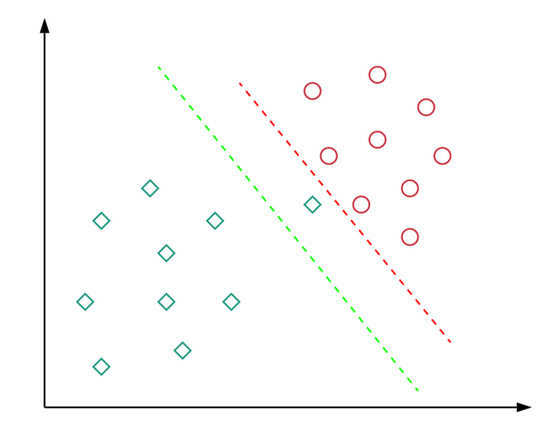
\includegraphics[height=0.5\textheight]{Images/softSVMseparable.png}
			
			\vspace*{0.5em}
			\footnotesize{\textcolor{MPTgrey}{Image tirée de l'article \href{https://towardsdatascience.com/support-vector-machines-soft-margin-formulation-and-kernel-trick-4c9729dc8efe}{\textit{Support Vector Machines — Soft Margin Formulation and Kernel Trick}} publié dans Towards Data Science}}
			
		\end{center}
		
	}	

	\end{frame}
%------------------------------------------------------------------------------------------
%------------------------------------------------------------------------------------------
\begin{frame}{Formulation duale}
	\only<1-2>{
		\vspace*{-0.7em}
			\begin{minipt}[1]{0.75}
		%\vspace*{-1em}
		%	\begin{minipt}[1]{0.99}
			%	\vspace*{0.1em}
			\textcolor{MPTred}{\large\textbf{Proposition}}\hfill \textcolor{MPTgrey}{SVM à marge souple}\\
			\vspace*{-1.1em}		
			\begin{valblock}{}
				Soit $\widehat{\alpha} = (\widehat{\alpha}_1, \dots,\widehat{\alpha}_n) \in \bbR^n$ qui vérifie
				\begin{equation}\label{eq:optim5}
					\begin{array}{lll}
						\widehat{\alpha}& =& \displaystyle \underset{\alpha=(\alpha_1,\dots,\alpha_n) \in \bbR^n}{\text{{arg}}\,\max}\,\, \sum_{i=1}^n \alpha_i  - \dfrac{1}{2} \sum_{i=1}^n \sum_{\ell=1}^n \alpha_i\alpha_\ell \ y_i y_\ell \  \left\langle x_i,x_\ell\right\rangle\\				
						&& \text{s.c.} \sum_{i=1}^n \alpha_i y_i = 0 \text{ et } 0 \leq \alpha_i \leq C \hsp \forall i \in \{1,\dots,n\}  
					\end{array}
				\end{equation}
				
				Alors le couple $(\widehat{w}, \widehat{b})$ défini par
				$$ \widehat{w}= \sum_{i=1}^n  \widehat{\alpha}_i y_i x_i \hsp \hsp \text{et} \hsp \hsp \widehat{b}= y_i-\sum_{j=1}^n \widehat{\alpha}_j y_j \langle x_j,x_i \rangle  \hsp \text{pour } (x_i,y_i) \text{ t.q. } 0<\widehat{\alpha}_i <C $$
				est identique à la solution donnée par l'équation \eqref{eq:optim4}
			\end{valblock}
			\textcolor{MPTgrey} {Preuve : section 10.2.2 d'\textit{\href{http://cazencott.info/dotclear/public/lectures/IntroML_Azencott.pdf}{Introduction au Machine Learning}} de Chloé-Agathe Azencott} \\[1em]
		\end{minipt}
		\begin{minipt}[1]{0.18}	
			
					\only<1>{
						
								Il est possible (mais rare) qu'il n'existe pas $i \in \{1,\dots,n\}$ tel que $0<\widehat{\alpha}_i <C$, dans ce cas, il est possible de prendre une valeur au hasard dans un certain intervalle pour $\widehat{b}$. Il est cependant plutôt conseillé de changer $C$ pour avoir $0<\widehat{\alpha}_i <C$

			}
		
			\only<2>{
			\textbf{\textcolor{MPTblue}{Classifieur SVM à marge souple}} \hsp  $ 
			\displaystyle \text{sign} \left[ \sum_{i =1}^n \alpha_i y_i \left\langle x_i,x \right\rangle  + \widehat{b} \right]$
		}
			\end{minipt}	
			%	\end{minipt}
	}
	\only<3->{
	\begin{itemize}
		\vspace{-1em}
		\item  Le problème défini par \eqref{eq:optim5} est un \textbf{problème d'optimisation convexe et quadratique}. \\[1em]
		
	\item \textbf{Interprétation géométrique} : les solutions $	\widehat{\alpha}$ et $(\widehat{w},\widehat{b})$ vérifient les \textit{conditions d'optimalité de Karush-Kuhn-Tucker} dont la \textit{condition d'écart complémentaire} qui stipule que, pour tout $i \in \llbracket1,n\rrbracket$, $\widehat{\alpha}_i \left[y_i\left(\langle\widehat{w}, x_i\rangle + \widehat{b}\right) - 1 + \xi_i\right] = 0$. \\[0.5em]
	
		
		\begin{itemize}
			\item[\ex] \hsp Si $x_i$ est \textit{au dessus} de $H_+$ pour $y_i=1$ et en dessous de $H_{-}$ pour $y_i=-1$,\\ \hsp \ie $y_i\left(\langle\widehat{w}, x_i\rangle + \widehat{b}\right) > 1$ alors $\xi_i=0$ et donc $\widehat{\alpha}_i=0$\\[1em]
			
			\item[\ex] \hsp Si $\widehat{\alpha}_i>0$ alors \\[0.5em]			
			\begin{itemize}
				\item[$\large \bullet$] Si $\xi_i =0$ alors $y_i\left(\langle\widehat{w}, x_i\rangle + \widehat{b}\right)=1$, \ie $x_i \in H_+$ si $y_i=1$ et $x_i \in H_-$ si $y_i=-1$; $x_i$ est donc un vecteur de support\\[1em]
				\item[$\large \bullet$]  Si $\xi_i \neq 0$ alors $x_i$ est un outlier. 
				%De plus, d'après les \textit{conditions d'optimalité de Karush-Kuhn-Tucker}, $\widehat{\alpha}_i^ = C$\\[1em]
			\end{itemize}
		\end{itemize}		
		La formulation duale permet d'identifier des vecteurs de support (pas forcément tous) et des outliers (pas forcément tous). Ce sont seulement ces vecteurs de support et outliers qui sont utilisés pour construire le classifieur à marge souple\\[1em]


	%		\item \textbf{\textcolor{MPTblue}{Classifieur SVM à marge rigide}}: \hsp  $f(x) = 
	%	\displaystyle \text{sign} \left[ \sum_{i =1}^n \alpha_i y_i \langle x_i,x\rangle  + \widehat{b} \right]$
\end{itemize}
		}
\end{frame}
%------------------------------------------------------------------------------------------
%------------------------------------------------------------------------------------------

\section{Le cas linéairement non séparable :\\[0.5em] SVM à noyau}
%------------------------------------------------------------------------------------------
%------------------------------------------------------------------------------------------
\begin{frame}{Problématique}
	\vspace*{-1em}
	\begin{center}		
		\begin{tikzpicture}
			\node (ref) [visible on=<1->] {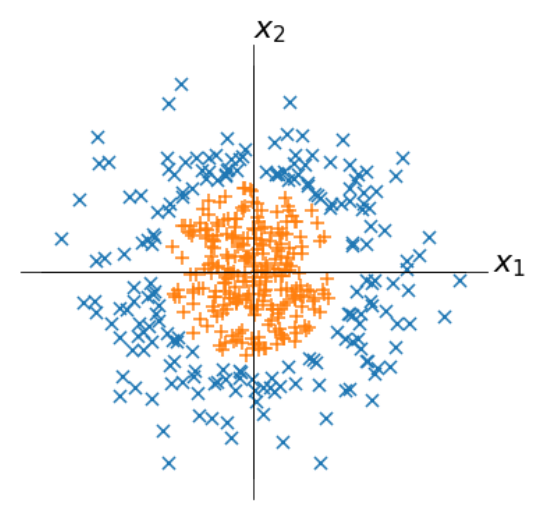
\includegraphics[width=0.4\textwidth,clip]{nonseparablecercle.png}};
			%\node (ref) [visible on=<2->] {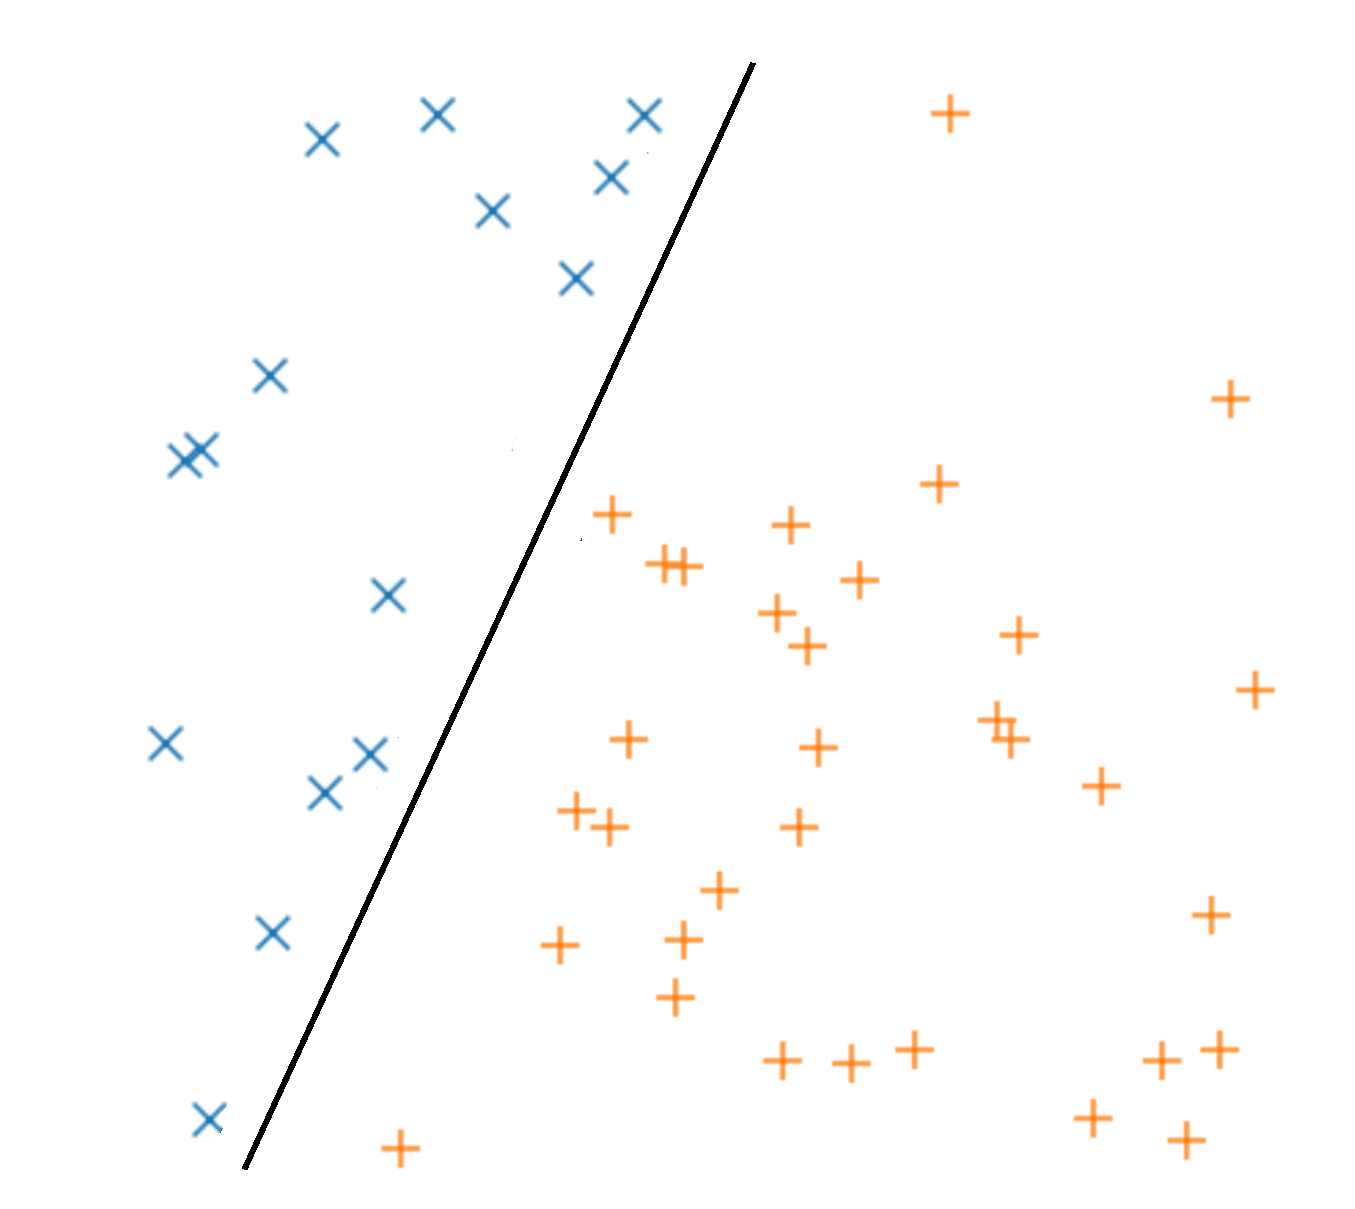
\includegraphics[width=0.4\textwidth,clip]{separabledroite.pdf}};
			%\node (wiki)[]  at([yshift = 13]ref.north) {Linéairement séparables};
			%
			\node (ref1) [right=of ref,visible on=<2>] {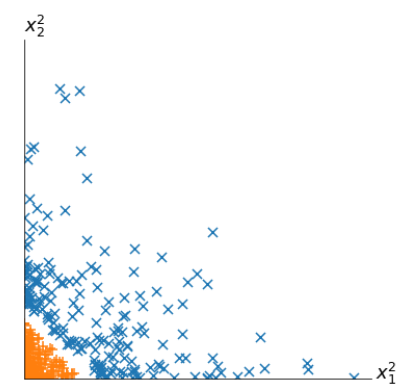
\includegraphics[width=0.4\textwidth,clip]{separabledim.png}};
			%\node (ref1) [right=of ref,visible on=<3>] {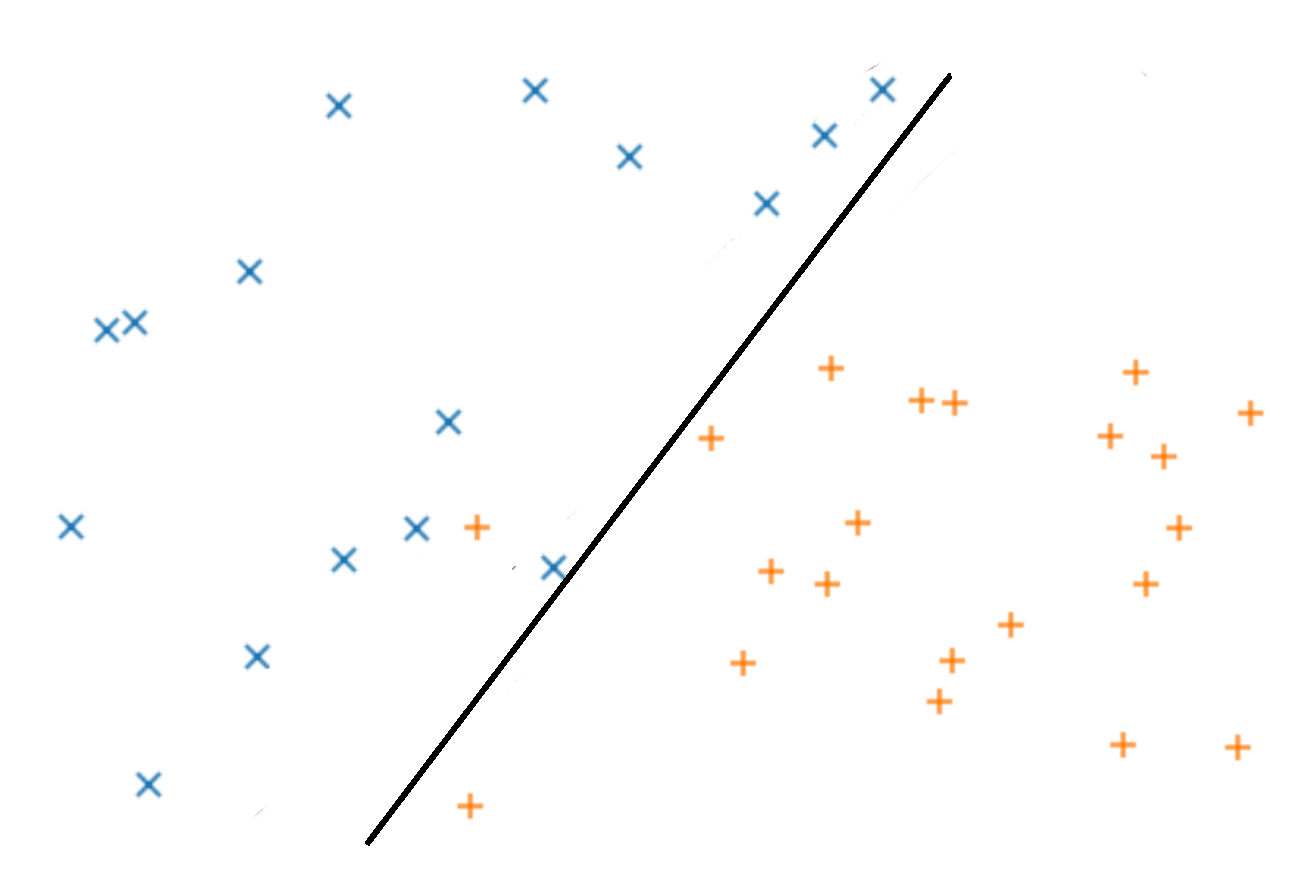
\includegraphics[width=0.4\textwidth,clip]{nonseparable1b.pdf}};
			%\node (ref1) [right=of ref,visible on=<4>] {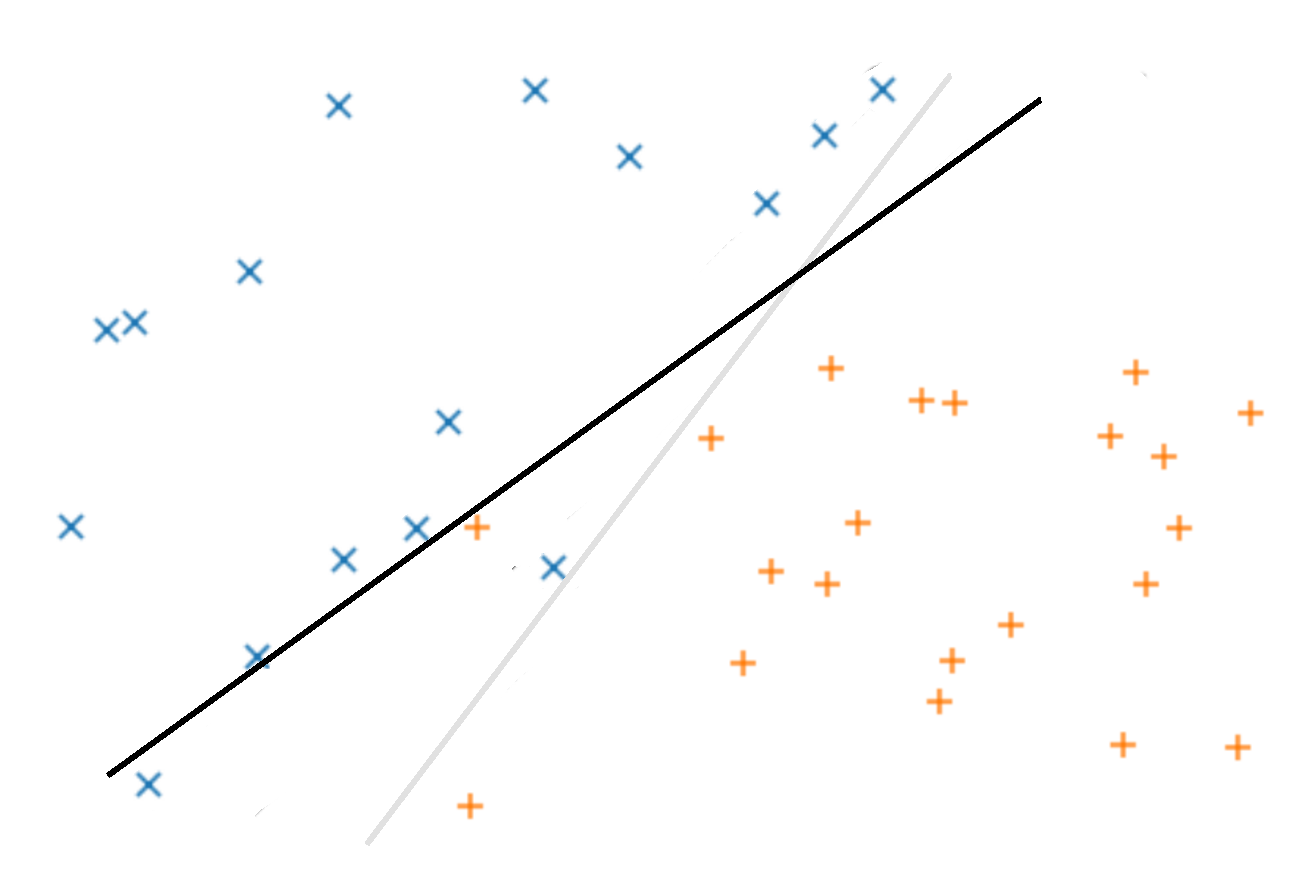
\includegraphics[width=0.4\textwidth,clip]{nonseparable2b.pdf}};
			%\node (ref1) [right=of ref,visible on=<5>] {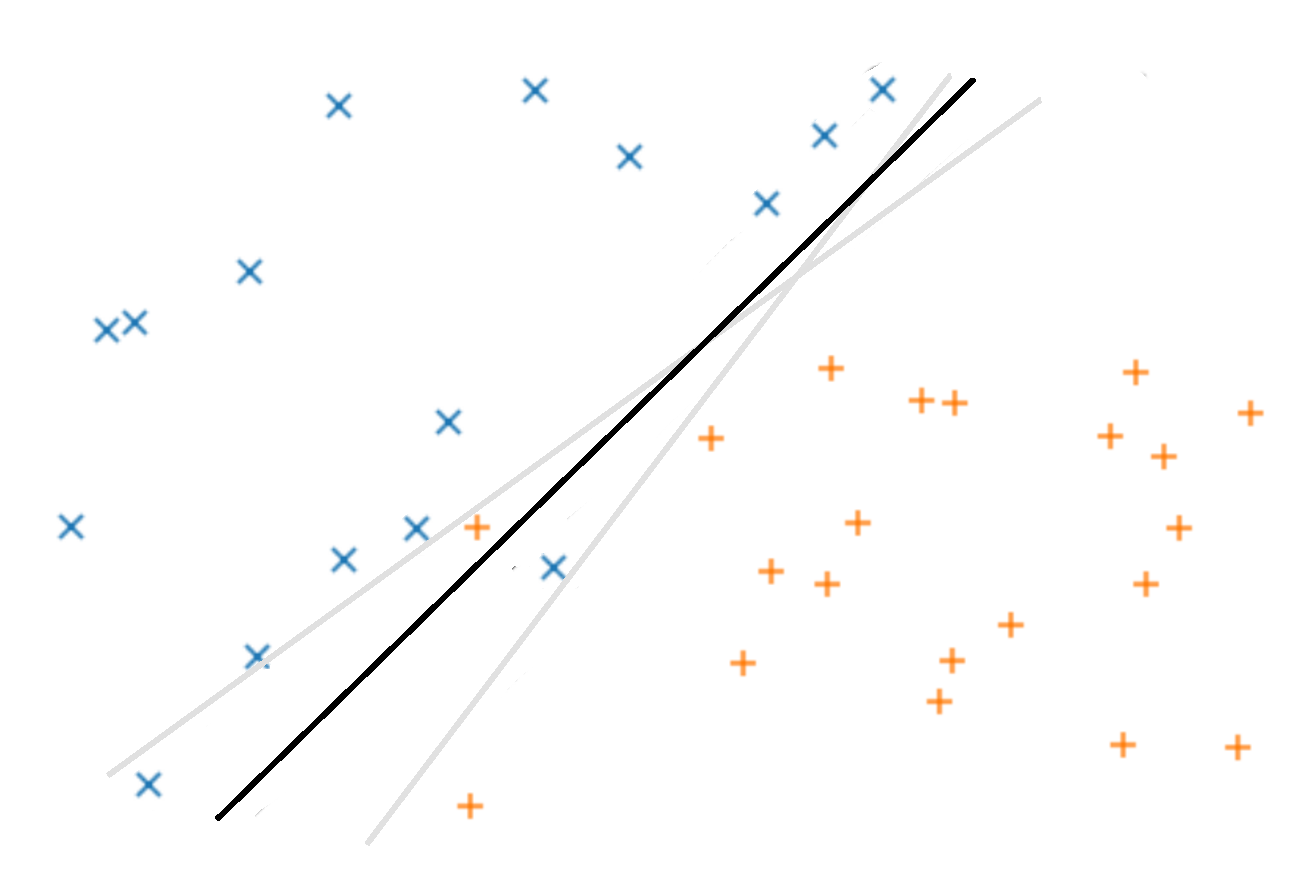
\includegraphics[width=0.4\textwidth,clip]{nonseparable3b.pdf}};
			\node (wiki1)[visible on=<2>]at([xshift = 22]ref1) {$\phi(x_1,x_2) \mapsto \left(x_1^2,x_2^2\right)$};
			%\node (wiki)[]  at([yshift = 27.5]ref1.north) {Non séparables linéairement};
			
		\end{tikzpicture}
		
	%	\vspace*{1.5em}
		\footnotesize{\textcolor{MPTgrey}{Tirée de l'ouvrage \textit{\href{http://cazencott.info/dotclear/public/lectures/IntroML_Azencott.pdf}{Introduction au Machine Learning}} de Chloé-Agathe Azencott} }\\
	\end{center}

\vspace*{1em}
			\begin{minipc}[0.06]{0.11}
			\warning
		\end{minipc}
		\begin{minipc}[0.93]{0.11}
			Les données ne sont pas séparables linéairement (même à quelques observations près)
		\end{minipc}
		\uncover<2>{
			\begin{minipc}[0.06]{0.15}
				%\begin{center}
				\raisebox{1.5mm}{\bclampe \xspace} 
			\end{minipc}
			\begin{minipc}[0.93]{0.15}
				On va transformer les données par une application $\phi : \X \to \H$   afin de les séparer linéairement dans l'espace de redescription $\H$ en utilisant une SVM à marge souple
			\end{minipc}
}
\end{frame}
%------------------------------------------------------------------------------------------
%------------------------------------------------------------------------------------------
\begin{frame}{Formulation duale}
	\only<1>{
		\vspace*{-1em}
		%	\begin{minipt}[1]{0.99}
			%	\vspace*{0.1em}
			\textcolor{MPTred}{\large\textbf{Problème duale}}\hfill \textcolor{MPTgrey}{SVM à marge souple sur données transformées}\\
			\vspace*{-0.2em}		
			\begin{valblock}{}
				On cherche $\widehat{\alpha} = (\widehat{\alpha}_1, \dots,\widehat{\alpha}_n) \in \bbR^n$ qui vérifie
				\begin{equation}\label{eq:optim6-bis}
					\begin{array}{lll}
						\widehat{\alpha}& =& \displaystyle \underset{\alpha=(\alpha_1,\dots,\alpha_n) \in \bbR^n}{\text{{arg}}\,\max}\,\, \sum_{i=1}^n \alpha_i  - \dfrac{1}{2} \sum_{i=1}^n \sum_{\ell=1}^n \alpha_i\alpha_\ell \ y_i y_\ell \  \left\langle \boldsymbol{\phi(x_i)},\boldsymbol{\phi(x_\ell)} \right\rangle\\				
						&& \text{s.c.} \sum_{i=1}^n \alpha_i y_i = 0 \text{ et } 0 \leq \alpha_i \leq C \hsp \forall i \in \{1,\dots,n\}  
					\end{array}
				\end{equation}
				
			avec $\widehat{w}$ défini comme précédemment (voir problème dual, SVM marge souple) et $\widehat{b}$ défini par
				$$ \widehat{b}= y_i-\sum_{j=1}^n \widehat{\alpha}_j y_j \left\langle \boldsymbol{\phi(x_j)},\boldsymbol{\phi(x_i)} \right\rangle  \hsp \text{pour } \text{pour } i \in\{1,\dots, n\} \text{ t.q. } 0<\widehat{\alpha}_i <C $$
				\end{valblock}
			
			%\textcolor{MPTgrey} {Preuve : section 10.2.2 d'\textit{\href{http://cazencott.info/dotclear/public/lectures/IntroML_Azencott.pdf}{Introduction au Machine Learning}} de Chloé-Agathe Azencott} \\[1em]
	\textbf{\textcolor{MPTblue}{Classifieur SVM à marge souple}} \hsp  $f(x) =  \displaystyle
\text{sign} \left[ \sum_{i =1}^n \alpha_i y_i \left\langle \boldsymbol{\phi(x_i)},\boldsymbol{\phi(x)}\right\rangle  + \widehat{b} \right]$
			
			%	\end{minipt}
	}
	
\end{frame}

%------------------------------------------------------------------------------------------
%------------------------------------------------------------------------------------------
\begin{frame}{L'astuce du noyau}
L'application $\phi : \X \to \H$ intervient dans le problème d'optimisation induit par \eqref{eq:optim6-bis} et dans l'expression du classifieur à marge souple uniquement via les produits scalaires
$$ \left\langle {\phi(x_j)},{\phi(x_i)} \right\rangle \hsp i,j \in \{1,\dots ,n\}$$

			\begin{minipc}[0.06]{0.11}
	\warning
\end{minipc}
\begin{minipc}[0.93]{0.07}
	La dimension de $\H$ peut être grande et donc le calcul de $ \left\langle {\phi(x_j)},{\phi(x_i)} \right\rangle$ coûteux
\end{minipc}
\vspace*{-1em}

\begin{minipc}[0.06]{0.1}
	%\begin{center}
	\raisebox{1.5mm}{\bclampe \xspace} 
\end{minipc}
\begin{minipc}[0.93]{0.15}
	Essayer de calculer $ \left\langle {\phi(x_j)},{\phi(x_i)} \right\rangle$ de manière plus efficace
\end{minipc}

\vspace*{1em}
	\textcolor{MPTblue}{\textbf{Ex.}} \hsp  $ \phi : x=(x_1,\dots,x_d) \in \bbR^d \mapsto (1,x_1,\dots,x_d,x_1x_1,x_1x_2,\dots,x_dx_d) \in \bbR^{1+d+d^2}$ 	
	$$ 
	\begin{array}{llll}
	\left\langle \phi(x),\phi(\tilde{x})\right\rangle &=& \displaystyle 1 + \sum_{i=1}^d x_i\tilde{x_i} + \sum_{i=1}^d\sum_{j=1}^d x_i\tilde{x_i}x_j\tilde{x_j} & \text{\textcolor{MPTgrey}{complexité algo.} } \color{MPTgrey} O(d^2)\\
	&= &1 + \langle x, \tilde{x} \rangle + \langle x, \tilde{x} \rangle^2 & \text{\textcolor{MPTgrey}{complexité algo.} } \color{MPTgrey} O(d)\\
	&=& K(x, \tilde{x})
	\end{array}
	$$


	
\end{frame}


%------------------------------------------------------------------------------------------
%------------------------------------------------------------------------------------------
\begin{frame}{L'astuce du noyau}
		\vspace*{-1em}
	Soit la fonction $K$, appelée noyau, définie par
	\vspace*{-1em}
	$$\begin{array}{rcl}
		 K: (x,\tilde{x}) \in \X \times \X &\mapsto & \left\langle{\phi(x)},{\phi(\tilde{x})} \right\rangle \in \bbR
	\end{array}$$	
	\bftitle{Astuce du noyau} \hfill $ \color{MPTgrey} i,j \in \{1,\dots,n\}$\\
	\vspace*{-0.2em}
	\begin{vblock}{}
	Au lieu de calculer $\phi(x_i)$ et $\phi(x_j)$ puis de calculer $\left\langle{\phi(x_i)},{\phi(x_j)} \right\rangle$, on calcule directement $K(x_i,x_j)$
	\end{vblock}
	\vspace*{-0.5em}
	
	\bftitle{Remarque} \hsp L'astuce du noyau intervient dans le cadre du problème\\ \phantom{\bftitle{Remarque} \hsp}d'optimisation duale\\[0.8em]
\begin{itemize}
	\item  \hsp Il est souvent plus efficace en terme de temps de calcul de calculer $K(x_i,x_j)$ \hsp plutôt que $\phi(x_i)$, $\phi(x_j)$ puis $\left\langle{\phi(x_i)},{\phi(x_j)}\right\rangle$\\[0.5em]
	
	\item \hsp Il n'y a pas besoin de connaître $\phi$ explicitement, il nous suffit juste de \hsp connaître le noyau $K$. Aussi, $K$ peut être choisi de manière arbitraire \hsp (hyperparamètre), du moment que l'existence de $\phi$ est garantie. \\[1.2em]
\end{itemize}

\bftitle{Question} \hsp Soit $K	: \X \times \X \to \bbR$. Qu'est-ce qui garantit qu'il existe $\phi : \X \to \H$\\\phantom{\bftitle{Question} \hsp}telle que $K(x, \tilde{x}) = \left\langle{\phi(x)},{\phi(\tilde{x})} \right\rangle$ ?
\end{frame}
%------------------------------------------------------------------------------------------
%------------------------------------------------------------------------------------------
\begin{frame}{Propriétés du noyau $\color{MPTblue} K$}
	\vspace*{-0.8em}
	\begin{minipt}[1]{0.78}
\textcolor{MPTblue}{\large\textbf{Définition}}\\
\vspace*{-1.1em}		
\begin{vblock}{}
	Soit une fonction $K : \X \times \X \mapsto \bbR $
	\begin{itemize}
		\item $K$ est dite \textbf{symétrique} si $K(x,\tilde{x}) = K(\tilde{x},x)$ pour tout $x, \tilde{x} \in \X$\\[0.5em]
		\item $K$ est dite \textbf{semi-définie positive} si 
		$$ \forall m \in \bbN, \forall x_1,\dots,x_m\in \X, \forall a_1,\dots,a_m \in \bbR \hsp \sum_{i=1}^m  \sum_{i=j}^m  a_ia_j \, K(x_i,x_j) \geq 0$$
		\vspace*{-1.5em}
	\end{itemize}
\end{vblock}

	\vspace*{-1em}
\textcolor{MPTred}{\large\textbf{Théorème}}\hfill \textcolor{MPTgrey}{Moore-Aronszajn}\\
\vspace*{-1.1em}		
\begin{valblock}{}
	Soit $K : \X \times \X \mapsto \bbR $ une fonction symétrique et semi-définie positive alors il existe un espace (de Hilbert) $\H$ et une application $\phi : \X \to \H$ telle que
	$$ \forall x, \tilde{x} \in \X \hsp K(x,\tilde{x}) =  \left\langle{\phi(x)},{\phi(\tilde{x})} \right\rangle$$
		\vspace*{-1.5em}
	\end{valblock}
	\vspace*{-1em}

\begin{minipc}[0.06]{0.1}
	%\begin{center}
	\raisebox{1.5mm}{\bclampe \xspace} 
\end{minipc}
\begin{minipc}[0.93]{0.07}
On choisit donc le noyau $K$ tel qu'il soit symétrique et semi-défini positif
\end{minipc}
\end{minipt}

\begin{minipt}[1]{0.2}
		\only<1>{
		\bftitle{Exercice} \hsp Écrire le noyau $K : (x,\tilde{x}) \in \bbR^d\times \bbR^d \mapsto \left( \left\langle x, \tilde{x} \right\rangle + c \right)^2$, $c\in \bbR_+$ sous\\\phantom{\bftitle{Exercice} \hsp}forme d'un produit scalaire $\left\langle \phi(x),\phi(\tilde{x}) \right\rangle$
	}
	\only<2>{
\bftitle{Remarque} \hsp Soit un noyau $K$ et des observations $x_1,\dots,x_n$. La matrice\\\phantom{\bftitle{Remarque} \hsp}$ M \in \bbR^{n\times n}$  définie par $M_{i,j} = K(x_i,x_j)$ est appelée \textit{matrice de Gram}
}
\end{minipt}

\end{frame}

%------------------------------------------------------------------------------------------
%------------------------------------------------------------------------------------------

\begin{frame}{Exemples de noyau}
Soit $x, \tilde{x} \in \bbR^d \times \bbR^d$\hfill $\color{MPTgrey}\|\cdot\|$ \textcolor{MPTgrey}{: dist. euclidienne}\\[1.5em]
\bftitle{Noyau linéaire} \hsp $K(x, \tilde{x}) =  \left\langle x, \tilde{x} \right\rangle$ \\[1.5em]

\bftitle{Noyau cosinus} \hsp $K(x, \tilde{x}) = \dfrac{ \left\langle x, \tilde{x} \right\rangle}{\|x\| \|\tilde{x}\|}$\\[1.5em]

\bftitle{Noyau quadratique} \hsp $K(x, \tilde{x}) = \left( \left\langle x, \tilde{x} \right\rangle + c \right)^2$ \hsp $c \in \bbR_+$\\[1.5em]

\bftitle{Noyau polynomial} \hsp $K(x, \tilde{x}) = \left( \left\langle x, \tilde{x} \right\rangle + c \right)^d$\hsp $c \in \bbR_+$, $d \in \bbN$\\[1.5em]

\bftitle{Noyau gaussien} \hsp $K(x, \tilde{x}) = \exp \left\{ -\dfrac{1}{2} (x-\tilde{x})^T \ \Sigma^{-1} \ (x-\tilde{x})\right\}$\\
\phantom{\bftitle{Noyau gaussien} \hsp}$\Sigma \in \bbR^{d\times d}$ matrice semi-définie positive\\[1.5em]

\bftitle{Noyau gaussien} \hsp $K(x, \tilde{x}) = \exp \left\{ -\dfrac{\|x-\tilde{x}\|^2}{2 \sigma^2} \right\} \hsp \sigma \in \bbR^*_+$\\[1.5em]

	
\end{frame}

%------------------------------------------------------------------------------------------
%------------------------------------------------------------------------------------------



%------------------------------------------------------------------------------------------
%------------------------------------------------------------------------------------------
\begin{frame}{Formulation duale avec le noyau}

		%\vspace*{-1em}
			\begin{minipt}[1]{0.7}
			%	\vspace*{0.1em}
			\textcolor{MPTred}{\large\textbf{Problème duale}}\hfill \textcolor{MPTgrey}{SVM à marge souple et à noyau}\\
			\vspace*{-1.1em}		
			\begin{valblock}{}
				On cherche $\widehat{\alpha} = (\widehat{\alpha}_1, \dots,\widehat{\alpha}_n) \in \bbR^n$ qui vérifie
				\begin{equation}\label{eq:optim6}
					\begin{array}{lll}
						\widehat{\alpha}& =& \displaystyle \underset{\alpha=(\alpha_1,\dots,\alpha_n) \in \bbR^n}{\text{{arg}}\,\max}\,\, \sum_{i=1}^n \alpha_i  - \dfrac{1}{2} \sum_{i=1}^n \sum_{\ell=1}^n \alpha_i\alpha_\ell \ y_i y_\ell \ \boldsymbol{K(x_i,x_\ell)} \\				
						&& \text{s.c.} \sum_{i=1}^n \alpha_i y_i = 0 \text{ et } 0 \leq \alpha_i \leq C \hsp \forall i \in \{1,\dots,n\}  
					\end{array}
				\end{equation}
				
				avec $\widehat{w}$ défini comme précédemment (voir problème dual, SVM marge souple) et $\widehat{b}$ défini par
				$$ \widehat{b}= y_i-\sum_{j=1}^n \widehat{\alpha}_j y_j  \boldsymbol{K(x_j,x_i)}  \hsp \text{pour } i \in\{1,\dots, n\} \text{ t.q. } 0<\widehat{\alpha}_i <C $$
			\end{valblock}
		\end{minipt}
	\begin{minipt}[1]{2.3}
			
		
				
						
			\only<1>{\textbf{Le paramètre $\boldsymbol{C}$ et le noyau $\boldsymbol{K}$ sont des hyperparamètres que l'utilisateur doit choisir}. Ce choix peut être guidé en comparant, pour différents noyaux $K$ et constantes $C$, les performances des modèles sur les données de validation}
			
			
			%\textcolor{MPTgrey} {Preuve : section 10.2.2 d'\textit{\href{http://cazencott.info/dotclear/public/lectures/IntroML_Azencott.pdf}{Introduction au Machine Learning}} de Chloé-Agathe Azencott} \\[1em]
		\only<2>{\textbf{\textcolor{MPTblue}{Classifieur SVM à marge souple}} \hsp  $f(x) =  \displaystyle
			\text{sign} \left[ \sum_{i =1}^n \widehat{\alpha}_i y_i  \boldsymbol{K(x_i,x)}  + \widehat{b} \right]$
		}
\end{minipt}
	
	
\end{frame}

%------------------------------------------------------------------------------------------
%------------------------------------------------------------------------------------------

%\begin{frame}{Remarques}
%%\begin{itemize}
%%\item SVM dans le cadre de la classification multi-classe, $\Y=\{1,\dots, C\}$\\[2em]
%%\item SVM dans le cadre de la régression $\Y = \bbR$\\[2em]
%%\item L’astuce du noyau s’applique aussi à d’autres algorithmes d’apprentissage linéaires, comme la régression ridge
%%\end{itemize}
%\end{frame}
%------------------------------------------------------------------------------------------
%------------------------------------------------------------------------------------------

\begin{frame}{Références}
	\begin{thebibliography}{2}
			\vspace{-1.8em}
			
	%	\bibitem{1} L.~Bel, J.N.~Bacro and C.~Lantuéjoul, \textcolor{black}{Assessing extremal dependence of environmental spatial fields,} \emph{Environmetrics}, 19(2):163-182, 2008
		
		\bibitem{pouet} C.A.~Azencot \textcolor{black}{{\href{http://cazencott.info/dotclear/public/lectures/IntroML_Azencott.pdf}{Introduction au Machine Learning}}}, \emph{Dunod},\\ ISBN : 978-2-10-084143-1\\[2em]
		
	%	\bibitem{CNP2006} D.~Cooley, P.~Naveau and P.~Poncet \textcolor{black}{Variograms for spatial max-stable random fields}, pages 370-390, \emph{Springer New-York}, 2006
		
		\bibitem{2} S.~Shalev-Shwartz and S.~Ben-David, \textcolor{black}{Understanding Machine Learning: From Theory to Algorithms,} \emph{Cambridge University Press}, DOI : 10.1017/CBO9781107298019, 2014\\[2em]
		%
	%	\bibitem{3} C.~Dombry, S.~Engelke, M.~Oesting (2016) \textcolor{black}{Exact simulation of max-stable processes}, \textit{Biometrika} 103(2):303–317
		
		\bibitem{E} T.~Hastie, R.~Tibshirani, and J.~Friedman. \textcolor{black}{The Elements of Statistical Learning}, \emph{Springer New York}, DOI : 10.1007/978-0-387-84858-7, 2009
		
		
		%
		%	\bibitem{4} R.A.~Fisher and L.H.C.~Tippett, \textcolor{black}{Limiting forms of the frequency distribution of the largest or smallest member of a sample,} \emph{Mathematical Proceedings of the Cambridge Philosophical Society}, 24(2):180-190, 1928\\[0.3em]
		%	
	\end{thebibliography}
	
\end{frame}
\end{document}
